\documentclass[twoside]{book}

% Packages required by doxygen
\usepackage{fixltx2e}
\usepackage{calc}
\usepackage{doxygen}
\usepackage[export]{adjustbox} % also loads graphicx
\usepackage{graphicx}
\usepackage[utf8]{inputenc}
\usepackage{makeidx}
\usepackage{multicol}
\usepackage{multirow}
\PassOptionsToPackage{warn}{textcomp}
\usepackage{textcomp}
\usepackage[nointegrals]{wasysym}
\usepackage[table]{xcolor}

% Font selection
\usepackage[T1]{fontenc}
\usepackage[scaled=.90]{helvet}
\usepackage{courier}
\usepackage{amssymb}
\usepackage{sectsty}
\renewcommand{\familydefault}{\sfdefault}
\allsectionsfont{%
  \fontseries{bc}\selectfont%
  \color{darkgray}%
}
\renewcommand{\DoxyLabelFont}{%
  \fontseries{bc}\selectfont%
  \color{darkgray}%
}
\newcommand{\+}{\discretionary{\mbox{\scriptsize$\hookleftarrow$}}{}{}}

% Page & text layout
\usepackage{geometry}
\geometry{%
  a4paper,%
  top=2.5cm,%
  bottom=2.5cm,%
  left=2.5cm,%
  right=2.5cm%
}
\tolerance=750
\hfuzz=15pt
\hbadness=750
\setlength{\emergencystretch}{15pt}
\setlength{\parindent}{0cm}
\setlength{\parskip}{3ex plus 2ex minus 2ex}
\makeatletter
\renewcommand{\paragraph}{%
  \@startsection{paragraph}{4}{0ex}{-1.0ex}{1.0ex}{%
    \normalfont\normalsize\bfseries\SS@parafont%
  }%
}
\renewcommand{\subparagraph}{%
  \@startsection{subparagraph}{5}{0ex}{-1.0ex}{1.0ex}{%
    \normalfont\normalsize\bfseries\SS@subparafont%
  }%
}
\makeatother

% Headers & footers
\usepackage{fancyhdr}
\pagestyle{fancyplain}
\fancyhead[LE]{\fancyplain{}{\bfseries\thepage}}
\fancyhead[CE]{\fancyplain{}{}}
\fancyhead[RE]{\fancyplain{}{\bfseries\leftmark}}
\fancyhead[LO]{\fancyplain{}{\bfseries\rightmark}}
\fancyhead[CO]{\fancyplain{}{}}
\fancyhead[RO]{\fancyplain{}{\bfseries\thepage}}
\fancyfoot[LE]{\fancyplain{}{}}
\fancyfoot[CE]{\fancyplain{}{}}
\fancyfoot[RE]{\fancyplain{}{\bfseries\scriptsize Generated by Doxygen }}
\fancyfoot[LO]{\fancyplain{}{\bfseries\scriptsize Generated by Doxygen }}
\fancyfoot[CO]{\fancyplain{}{}}
\fancyfoot[RO]{\fancyplain{}{}}
\renewcommand{\footrulewidth}{0.4pt}
\renewcommand{\chaptermark}[1]{%
  \markboth{#1}{}%
}
\renewcommand{\sectionmark}[1]{%
  \markright{\thesection\ #1}%
}

% Indices & bibliography
\usepackage{natbib}
\usepackage[titles]{tocloft}
\setcounter{tocdepth}{3}
\setcounter{secnumdepth}{5}
\makeindex

% Hyperlinks (required, but should be loaded last)
\usepackage{ifpdf}
\ifpdf
  \usepackage[pdftex,pagebackref=true]{hyperref}
\else
  \usepackage[ps2pdf,pagebackref=true]{hyperref}
\fi
\hypersetup{%
  colorlinks=true,%
  linkcolor=blue,%
  citecolor=blue,%
  unicode%
}

% Custom commands
\newcommand{\clearemptydoublepage}{%
  \newpage{\pagestyle{empty}\cleardoublepage}%
}

\usepackage{caption}
\captionsetup{labelsep=space,justification=centering,font={bf},singlelinecheck=off,skip=4pt,position=top}

%===== C O N T E N T S =====

\begin{document}

% Titlepage & ToC
\hypersetup{pageanchor=false,
             bookmarksnumbered=true,
             pdfencoding=unicode
            }
\pagenumbering{alph}
\begin{titlepage}
\vspace*{7cm}
\begin{center}%
{\Large Pilot Engine \\[1ex]\large 0.\+1 }\\
\vspace*{1cm}
{\large Generated by Doxygen 1.8.14}\\
\end{center}
\end{titlepage}
\clearemptydoublepage
\pagenumbering{roman}
\tableofcontents
\clearemptydoublepage
\pagenumbering{arabic}
\hypersetup{pageanchor=true}

%--- Begin generated contents ---
\chapter{Module Index}
\section{Modules}
Here is a list of all modules\+:\begin{DoxyCompactList}
\item \contentsline{section}{Getters}{\pageref{group___getters}}{}
\item \contentsline{section}{functions that are supposed to be overwritten.}{\pageref{group___virtual}}{}
\end{DoxyCompactList}

\chapter{Hierarchical Index}
\section{Class Hierarchy}
This inheritance list is sorted roughly, but not completely, alphabetically\+:\begin{DoxyCompactList}
\item \contentsline{section}{piolot\+:\+:Asset\+Manager}{\pageref{classpiolot_1_1_asset_manager}}{}
\item \contentsline{section}{piolot\+:\+:Bounding\+Box}{\pageref{classpiolot_1_1_bounding_box}}{}
\item \contentsline{section}{piolot\+:\+:Camera}{\pageref{classpiolot_1_1_camera}}{}
\item \contentsline{section}{piolot\+:\+:Camera\+Saving\+To\+Stream}{\pageref{structpiolot_1_1_camera_saving_to_stream}}{}
\item \contentsline{section}{piolot\+:\+:Entity}{\pageref{classpiolot_1_1_entity}}{}
\begin{DoxyCompactList}
\item \contentsline{section}{piolot\+:\+:Terrain}{\pageref{classpiolot_1_1_terrain}}{}
\end{DoxyCompactList}
\item \contentsline{section}{piolot\+:\+:G\+L\+Shader}{\pageref{classpiolot_1_1_g_l_shader}}{}
\item \contentsline{section}{piolot\+:\+:Grid}{\pageref{classpiolot_1_1_grid}}{}
\item \contentsline{section}{piolot\+:\+:Im\+Gui\+Control\+Variables}{\pageref{structpiolot_1_1_im_gui_control_variables}}{}
\item \contentsline{section}{piolot\+:\+:Im\+Gui\+Log}{\pageref{structpiolot_1_1_im_gui_log}}{}
\item \contentsline{section}{piolot\+:\+:Logging\+Manager}{\pageref{classpiolot_1_1_logging_manager}}{}
\item \contentsline{section}{piolot\+:\+:Map\+Tile}{\pageref{classpiolot_1_1_map_tile}}{}
\item \contentsline{section}{piolot\+:\+:Mesh}{\pageref{classpiolot_1_1_mesh}}{}
\item \contentsline{section}{piolot\+:\+:Object}{\pageref{classpiolot_1_1_object}}{}
\item \contentsline{section}{piolot\+:\+:Ray}{\pageref{classpiolot_1_1_ray}}{}
\item \contentsline{section}{piolot\+:\+:Scene}{\pageref{classpiolot_1_1_scene}}{}
\begin{DoxyCompactList}
\item \contentsline{section}{piolot\+:\+:Test\+Scene}{\pageref{classpiolot_1_1_test_scene}}{}
\end{DoxyCompactList}
\item \contentsline{section}{piolot\+:\+:Terrain\+Vertex\+Data}{\pageref{structpiolot_1_1_terrain_vertex_data}}{}
\item Test\begin{DoxyCompactList}
\item \contentsline{section}{All\+Tests}{\pageref{class_all_tests}}{}
\end{DoxyCompactList}
\item \contentsline{section}{piolot\+:\+:Texture}{\pageref{classpiolot_1_1_texture}}{}
\item \contentsline{section}{piolot\+:\+:Vertex\+Data}{\pageref{structpiolot_1_1_vertex_data}}{}
\item \contentsline{section}{All\+Tests\+:\+:Vertex\+Data\+Test\+Good}{\pageref{struct_all_tests_1_1_vertex_data_test_good}}{}
\item \contentsline{section}{piolot\+:\+:Viewport\+Details}{\pageref{structpiolot_1_1_viewport_details}}{}
\item \contentsline{section}{Window}{\pageref{class_window}}{}
\end{DoxyCompactList}

\chapter{Class Index}
\section{Class List}
Here are the classes, structs, unions and interfaces with brief descriptions\+:\begin{DoxyCompactList}
\item\contentsline{section}{\mbox{\hyperlink{class_all_tests}{All\+Tests}} }{\pageref{class_all_tests}}{}
\item\contentsline{section}{\mbox{\hyperlink{classpiolot_1_1_asset_manager}{piolot\+::\+Asset\+Manager}} \\*The Singleton class that holds all the data for Shaders, Textures and Objects }{\pageref{classpiolot_1_1_asset_manager}}{}
\item\contentsline{section}{\mbox{\hyperlink{classpiolot_1_1_bounding_box}{piolot\+::\+Bounding\+Box}} \\*This class is used to create a simple cuboid around the Objects as a Bounding Box }{\pageref{classpiolot_1_1_bounding_box}}{}
\item\contentsline{section}{\mbox{\hyperlink{classpiolot_1_1_camera}{piolot\+::\+Camera}} }{\pageref{classpiolot_1_1_camera}}{}
\item\contentsline{section}{\mbox{\hyperlink{structpiolot_1_1_camera_saving_to_stream}{piolot\+::\+Camera\+Saving\+To\+Stream}} }{\pageref{structpiolot_1_1_camera_saving_to_stream}}{}
\item\contentsline{section}{\mbox{\hyperlink{classpiolot_1_1_entity}{piolot\+::\+Entity}} }{\pageref{classpiolot_1_1_entity}}{}
\item\contentsline{section}{\mbox{\hyperlink{classpiolot_1_1_g_l_shader}{piolot\+::\+G\+L\+Shader}} \\*The Class that is used to load shaders in Open\+GL }{\pageref{classpiolot_1_1_g_l_shader}}{}
\item\contentsline{section}{\mbox{\hyperlink{classpiolot_1_1_grid}{piolot\+::\+Grid}} }{\pageref{classpiolot_1_1_grid}}{}
\item\contentsline{section}{\mbox{\hyperlink{structpiolot_1_1_im_gui_control_variables}{piolot\+::\+Im\+Gui\+Control\+Variables}} }{\pageref{structpiolot_1_1_im_gui_control_variables}}{}
\item\contentsline{section}{\mbox{\hyperlink{structpiolot_1_1_im_gui_log}{piolot\+::\+Im\+Gui\+Log}} }{\pageref{structpiolot_1_1_im_gui_log}}{}
\item\contentsline{section}{\mbox{\hyperlink{classpiolot_1_1_logging_manager}{piolot\+::\+Logging\+Manager}} }{\pageref{classpiolot_1_1_logging_manager}}{}
\item\contentsline{section}{\mbox{\hyperlink{classpiolot_1_1_map_tile}{piolot\+::\+Map\+Tile}} }{\pageref{classpiolot_1_1_map_tile}}{}
\item\contentsline{section}{\mbox{\hyperlink{classpiolot_1_1_mesh}{piolot\+::\+Mesh}} }{\pageref{classpiolot_1_1_mesh}}{}
\item\contentsline{section}{\mbox{\hyperlink{classpiolot_1_1_object}{piolot\+::\+Object}} }{\pageref{classpiolot_1_1_object}}{}
\item\contentsline{section}{\mbox{\hyperlink{classpiolot_1_1_ray}{piolot\+::\+Ray}} }{\pageref{classpiolot_1_1_ray}}{}
\item\contentsline{section}{\mbox{\hyperlink{classpiolot_1_1_scene}{piolot\+::\+Scene}} }{\pageref{classpiolot_1_1_scene}}{}
\item\contentsline{section}{\mbox{\hyperlink{classpiolot_1_1_terrain}{piolot\+::\+Terrain}} }{\pageref{classpiolot_1_1_terrain}}{}
\item\contentsline{section}{\mbox{\hyperlink{structpiolot_1_1_terrain_vertex_data}{piolot\+::\+Terrain\+Vertex\+Data}} }{\pageref{structpiolot_1_1_terrain_vertex_data}}{}
\item\contentsline{section}{\mbox{\hyperlink{classpiolot_1_1_test_scene}{piolot\+::\+Test\+Scene}} }{\pageref{classpiolot_1_1_test_scene}}{}
\item\contentsline{section}{\mbox{\hyperlink{classpiolot_1_1_texture}{piolot\+::\+Texture}} }{\pageref{classpiolot_1_1_texture}}{}
\item\contentsline{section}{\mbox{\hyperlink{structpiolot_1_1_vertex_data}{piolot\+::\+Vertex\+Data}} }{\pageref{structpiolot_1_1_vertex_data}}{}
\item\contentsline{section}{\mbox{\hyperlink{struct_all_tests_1_1_vertex_data_test_good}{All\+Tests\+::\+Vertex\+Data\+Test\+Good}} }{\pageref{struct_all_tests_1_1_vertex_data_test_good}}{}
\item\contentsline{section}{\mbox{\hyperlink{structpiolot_1_1_viewport_details}{piolot\+::\+Viewport\+Details}} }{\pageref{structpiolot_1_1_viewport_details}}{}
\item\contentsline{section}{\mbox{\hyperlink{class_window}{Window}} \\*\mbox{\hyperlink{class_window}{Window}} Class. Initialize this for opening the window. Cleanup to exit }{\pageref{class_window}}{}
\end{DoxyCompactList}

\chapter{Module Documentation}
\hypertarget{group___getters}{}\section{Getters}
\label{group___getters}\index{Getters@{Getters}}
\subsection*{Modules}
\begin{DoxyCompactItemize}
\item 
\mbox{\hyperlink{group___setters}{Setters}}
\end{DoxyCompactItemize}
\subsection*{Functions}
\begin{DoxyCompactItemize}
\item 
\mbox{\Hypertarget{group___getters_ga1534921bb22645320614b4cf02268906}\label{group___getters_ga1534921bb22645320614b4cf02268906}} 
const glm\+::vec3 \& {\bfseries piolot\+::\+Bounding\+Box\+::\+Get\+Minimum\+Point} () const
\item 
\mbox{\Hypertarget{group___getters_gafd9222c8fb47c5484c873ace9d66a37d}\label{group___getters_gafd9222c8fb47c5484c873ace9d66a37d}} 
const glm\+::vec3 \& {\bfseries piolot\+::\+Bounding\+Box\+::\+Get\+Maximum\+Point} () const
\item 
\mbox{\Hypertarget{group___getters_ga57651f343f21133fc6c89c8c5619ed84}\label{group___getters_ga57651f343f21133fc6c89c8c5619ed84}} 
unsigned int {\bfseries piolot\+::\+Bounding\+Box\+::\+Get\+Vertices\+Size} () const
\item 
\mbox{\hyperlink{group___getters_ga699e27e8e646be7a0a47f89abb35778d}{piolot\+::\+Bounding\+Box\+::\+Bounding\+Box}} (glm\+::vec3 \+\_\+minimum\+Point=glm\+::vec3(-\/0.\+2f, -\/0.\+2f, -\/0.\+2f), glm\+::vec3 \+\_\+maximum\+Point=glm\+::vec3(0.\+2f, 0.\+2f, 0.\+2f))
\begin{DoxyCompactList}\small\item\em Constructor. \end{DoxyCompactList}\item 
bool \mbox{\hyperlink{group___getters_ga552fcdb461cdc71c5da0fed7b486246d}{piolot\+::\+Bounding\+Box\+::\+Check\+For\+Collision\+With\+Ray}} (const glm\+::mat4 \+\_\+model\+Matrix, const glm\+::vec3 \+\_\+scale, const glm\+::vec3 \+\_\+ray\+Origin, const glm\+::vec3 \+\_\+ray\+Direction, float \&\+\_\+intersection\+Distance) const
\begin{DoxyCompactList}\small\item\em Check if the Bounding Box Collides with the \mbox{\hyperlink{classpiolot_1_1_ray}{Ray}}. \end{DoxyCompactList}\item 
void \mbox{\hyperlink{group___getters_ga3ef9f966674be7fa0448d388b7a3d776}{piolot\+::\+Bounding\+Box\+::\+Render}} (glm\+::vec3 \+\_\+colour)
\begin{DoxyCompactList}\small\item\em Render the Bounding Box. \end{DoxyCompactList}\item 
\mbox{\Hypertarget{group___getters_ga77d5347666653b9a20c389e0e412f700}\label{group___getters_ga77d5347666653b9a20c389e0e412f700}} 
unsigned {\bfseries Window\+::\+Get\+Width} ()
\item 
\mbox{\Hypertarget{group___getters_ga19c8d97415b163e5f641388f1d537085}\label{group___getters_ga19c8d97415b163e5f641388f1d537085}} 
unsigned {\bfseries Window\+::\+Get\+Height} ()
\item 
\mbox{\Hypertarget{group___getters_gae66865d49d16710c1cb11fd39ab7564f}\label{group___getters_gae66865d49d16710c1cb11fd39ab7564f}} 
std\+::string {\bfseries Window\+::\+Get\+Title} () const
\item 
\mbox{\Hypertarget{group___getters_gacd18a545a32f73ae1dc0c1bd00573f20}\label{group___getters_gacd18a545a32f73ae1dc0c1bd00573f20}} 
bool {\bfseries Window\+::\+Is\+Glad\+Init} () const
\item 
\mbox{\Hypertarget{group___getters_ga84c80356e911db086098e29e8a870829}\label{group___getters_ga84c80356e911db086098e29e8a870829}} 
bool {\bfseries Window\+::\+Is\+Glfw\+Init} () const
\item 
\mbox{\Hypertarget{group___getters_gad7e49197526473b23c01ecc9cd2292d2}\label{group___getters_gad7e49197526473b23c01ecc9cd2292d2}} 
G\+L\+F\+Wwindow $\ast$ {\bfseries Window\+::\+Get\+Window} () const
\item 
void \mbox{\hyperlink{group___getters_gac825ddc0aeda29fae94c5fc910f3f04d}{Window\+::\+Update\+Frame\+Size}} ()
\begin{DoxyCompactList}\small\item\em Updates the Class\textquotesingle{}s width and height with the G\+L\+FW Frame Buffer Width and Height. \end{DoxyCompactList}\item 
\mbox{\Hypertarget{group___getters_ga6703058dead0231b089862ad1e226c70}\label{group___getters_ga6703058dead0231b089862ad1e226c70}} 
void {\bfseries Window\+::\+Handle\+Input} () const
\item 
\mbox{\Hypertarget{group___getters_ga72708934a1134a2ad9729f45719902a7}\label{group___getters_ga72708934a1134a2ad9729f45719902a7}} 
bool {\bfseries Window\+::\+Is\+Key\+Pressed} (unsigned int \+\_\+key\+Code) const
\item 
\mbox{\Hypertarget{group___getters_ga4000d4a6212d66cb1b14023cfb68c3a0}\label{group___getters_ga4000d4a6212d66cb1b14023cfb68c3a0}} 
bool {\bfseries Window\+::\+Is\+Key\+Pressed\+And\+Released} (unsigned int \+\_\+key\+Code) const
\item 
\mbox{\Hypertarget{group___getters_ga78186413fc84fbb83f1c5c8a230d45fa}\label{group___getters_ga78186413fc84fbb83f1c5c8a230d45fa}} 
bool {\bfseries Window\+::\+Is\+Key\+Pressed\+Or\+Held} (const unsigned int \+\_\+keycode) const
\item 
\mbox{\Hypertarget{group___getters_ga2d13c2ec079ed3f8e907969781217c93}\label{group___getters_ga2d13c2ec079ed3f8e907969781217c93}} 
bool {\bfseries Window\+::\+Is\+Key\+Held} (unsigned int \+\_\+key\+Code) const
\item 
\mbox{\Hypertarget{group___getters_ga174de5939a61138e7c3cfe0136716f01}\label{group___getters_ga174de5939a61138e7c3cfe0136716f01}} 
bool {\bfseries Window\+::\+Is\+Mouse\+Button\+Pressed} (unsigned int \+\_\+button) const
\item 
void \mbox{\hyperlink{group___getters_ga65b02b0e52540d4c2c9d13689f4ec45a}{Window\+::\+Get\+Mouse\+Position}} (double \&x, double \&y) const
\begin{DoxyCompactList}\small\item\em Function to get the Mouse Position, to a couple of variables. \end{DoxyCompactList}\item 
\mbox{\Hypertarget{group___getters_ga86a9ed5f891a93f0c3c44d8577be4e71}\label{group___getters_ga86a9ed5f891a93f0c3c44d8577be4e71}} 
void {\bfseries Window\+::\+Update} (const float \+\_\+deltatime)
\item 
\mbox{\Hypertarget{group___getters_gab0d4c2fa778638e6fde90fc221124384}\label{group___getters_gab0d4c2fa778638e6fde90fc221124384}} 
static void \mbox{\hyperlink{group___getters_gab0d4c2fa778638e6fde90fc221124384}{Window\+::\+Clean\+Up}} ()
\begin{DoxyCompactList}\small\item\em Calls G\+L\+F\+W\+Terminate. \end{DoxyCompactList}\end{DoxyCompactItemize}
\subsection*{Variables}
\begin{DoxyCompactItemize}
\item 
\mbox{\Hypertarget{group___getters_ga7e9389c2d0e9f90f10422f86be7d22d8}\label{group___getters_ga7e9389c2d0e9f90f10422f86be7d22d8}} 
key\+\_\+bool \mbox{\hyperlink{group___getters_ga7e9389c2d0e9f90f10422f86be7d22d8}{Window\+::keys}} \mbox{[}M\+A\+X\+\_\+\+K\+E\+YS\mbox{]} \{\}
\begin{DoxyCompactList}\small\item\em The keys and their current state. \end{DoxyCompactList}\item 
\mbox{\Hypertarget{group___getters_gaa0adc9c4e183ccaa355928059359fe9a}\label{group___getters_gaa0adc9c4e183ccaa355928059359fe9a}} 
key\+\_\+bool \mbox{\hyperlink{group___getters_gaa0adc9c4e183ccaa355928059359fe9a}{Window\+::prev\+Keys}} \mbox{[}M\+A\+X\+\_\+\+K\+E\+YS\mbox{]} \{\}
\begin{DoxyCompactList}\small\item\em The Keys and their Previous State. \end{DoxyCompactList}\item 
\mbox{\Hypertarget{group___getters_gaf219ad727d87f6f2d0d34c0d165ec065}\label{group___getters_gaf219ad727d87f6f2d0d34c0d165ec065}} 
key\+\_\+bool \mbox{\hyperlink{group___getters_gaf219ad727d87f6f2d0d34c0d165ec065}{Window\+::mouse\+Buttons}} \mbox{[}M\+A\+X\+\_\+\+B\+U\+T\+T\+O\+NS\mbox{]} = \{ key\+\_\+inactive \}
\begin{DoxyCompactList}\small\item\em The Mouse buttons current state. \end{DoxyCompactList}\item 
\mbox{\Hypertarget{group___getters_ga89e8b6c9ffa84a095ec76cf1b29b5f94}\label{group___getters_ga89e8b6c9ffa84a095ec76cf1b29b5f94}} 
key\+\_\+bool \mbox{\hyperlink{group___getters_ga89e8b6c9ffa84a095ec76cf1b29b5f94}{Window\+::prev\+Mouse\+Buttons}} \mbox{[}M\+A\+X\+\_\+\+B\+U\+T\+T\+O\+NS\mbox{]} = \{ key\+\_\+inactive \}
\begin{DoxyCompactList}\small\item\em The Mouse buttons Previous state. \end{DoxyCompactList}\item 
\mbox{\Hypertarget{group___getters_gad50401a5c3c350b562b9577106e60fb0}\label{group___getters_gad50401a5c3c350b562b9577106e60fb0}} 
double \mbox{\hyperlink{group___getters_gad50401a5c3c350b562b9577106e60fb0}{Window\+::prev\+MouseX}} \{ 0.\+0 \}
\begin{DoxyCompactList}\small\item\em Mouse X Position in the Previous frame. \end{DoxyCompactList}\item 
\mbox{\Hypertarget{group___getters_gaf4a58a8da45b8aeeb36dbcae237bcef4}\label{group___getters_gaf4a58a8da45b8aeeb36dbcae237bcef4}} 
double \mbox{\hyperlink{group___getters_gaf4a58a8da45b8aeeb36dbcae237bcef4}{Window\+::prev\+MouseY}} \{ 0.\+0 \}
\begin{DoxyCompactList}\small\item\em Mouse Y Position in the Previous frame. \end{DoxyCompactList}\item 
\mbox{\Hypertarget{group___getters_ga68f752a9e5c04cf32a50b169df0de609}\label{group___getters_ga68f752a9e5c04cf32a50b169df0de609}} 
double \mbox{\hyperlink{group___getters_ga68f752a9e5c04cf32a50b169df0de609}{Window\+::mouseX}} \{ 0.\+0 \}
\begin{DoxyCompactList}\small\item\em Mouse X Position in the Current Frame. \end{DoxyCompactList}\item 
\mbox{\Hypertarget{group___getters_ga9f5f64a77451ba45212dab398f7b9dac}\label{group___getters_ga9f5f64a77451ba45212dab398f7b9dac}} 
double \mbox{\hyperlink{group___getters_ga9f5f64a77451ba45212dab398f7b9dac}{Window\+::mouseY}} \{ 0.\+0 \}
\begin{DoxyCompactList}\small\item\em Mouse Y Positin in the Current Frame. \end{DoxyCompactList}\item 
\mbox{\Hypertarget{group___getters_ga93b50aa557f493c5589af5dcc8f74c4a}\label{group___getters_ga93b50aa557f493c5589af5dcc8f74c4a}} 
double \mbox{\hyperlink{group___getters_ga93b50aa557f493c5589af5dcc8f74c4a}{Window\+::mouse\+OffsetX}} \{ 0.\+0 \}
\begin{DoxyCompactList}\small\item\em Mouse X offset from the last frame. \end{DoxyCompactList}\item 
\mbox{\Hypertarget{group___getters_ga22d84e6f9e9c7e283f303798b630c733}\label{group___getters_ga22d84e6f9e9c7e283f303798b630c733}} 
double \mbox{\hyperlink{group___getters_ga22d84e6f9e9c7e283f303798b630c733}{Window\+::mouse\+OffsetY}} \{ 0.\+0 \}
\begin{DoxyCompactList}\small\item\em Mouse Y offset from the last frame. \end{DoxyCompactList}\end{DoxyCompactItemize}


\subsection{Detailed Description}
Getters 

\subsection{Function Documentation}
\mbox{\Hypertarget{group___getters_ga699e27e8e646be7a0a47f89abb35778d}\label{group___getters_ga699e27e8e646be7a0a47f89abb35778d}} 
\index{Getters@{Getters}!Bounding\+Box@{Bounding\+Box}}
\index{Bounding\+Box@{Bounding\+Box}!Getters@{Getters}}
\subsubsection{\texorpdfstring{Bounding\+Box()}{BoundingBox()}}
{\footnotesize\ttfamily piolot\+::\+Bounding\+Box\+::\+Bounding\+Box (\begin{DoxyParamCaption}\item[{glm\+::vec3}]{\+\_\+minimum\+Point = {\ttfamily glm\+:\+:vec3(-\/0.2f,~-\/0.2f,~-\/0.2f)},  }\item[{glm\+::vec3}]{\+\_\+maximum\+Point = {\ttfamily glm\+:\+:vec3(0.2f,~0.2f,~0.2f)} }\end{DoxyParamCaption})\hspace{0.3cm}{\ttfamily [explicit]}}



Constructor. 


\begin{DoxyParams}{Parameters}
{\em \+\_\+minimum\+Point} & Min Point \\
\hline
{\em \+\_\+maximum\+Point} & Max Point \\
\hline
\end{DoxyParams}
\mbox{\Hypertarget{group___getters_ga552fcdb461cdc71c5da0fed7b486246d}\label{group___getters_ga552fcdb461cdc71c5da0fed7b486246d}} 
\index{Getters@{Getters}!Check\+For\+Collision\+With\+Ray@{Check\+For\+Collision\+With\+Ray}}
\index{Check\+For\+Collision\+With\+Ray@{Check\+For\+Collision\+With\+Ray}!Getters@{Getters}}
\subsubsection{\texorpdfstring{Check\+For\+Collision\+With\+Ray()}{CheckForCollisionWithRay()}}
{\footnotesize\ttfamily bool piolot\+::\+Bounding\+Box\+::\+Check\+For\+Collision\+With\+Ray (\begin{DoxyParamCaption}\item[{const glm\+::mat4}]{\+\_\+model\+Matrix,  }\item[{const glm\+::vec3}]{\+\_\+scale,  }\item[{const glm\+::vec3}]{\+\_\+ray\+Origin,  }\item[{const glm\+::vec3}]{\+\_\+ray\+Direction,  }\item[{float \&}]{\+\_\+intersection\+Distance }\end{DoxyParamCaption}) const}



Check if the Bounding Box Collides with the \mbox{\hyperlink{classpiolot_1_1_ray}{Ray}}. 


\begin{DoxyParams}{Parameters}
{\em \+\_\+model\+Matrix} & Model Matrix of the \mbox{\hyperlink{classpiolot_1_1_entity}{Entity}} \\
\hline
{\em \+\_\+scale} & Scale of the \mbox{\hyperlink{classpiolot_1_1_entity}{Entity}}. \\
\hline
{\em \+\_\+ray\+Origin} & \mbox{\hyperlink{classpiolot_1_1_ray}{Ray}} origin \\
\hline
{\em \+\_\+ray\+Direction} & \mbox{\hyperlink{classpiolot_1_1_ray}{Ray}} Direction \\
\hline
{\em \+\_\+intersection\+Distance} & Return the Intersection Distance \\
\hline
\end{DoxyParams}
\begin{DoxyReturn}{Returns}
If Intersected, return true. Else, False. 
\end{DoxyReturn}
\mbox{\Hypertarget{group___getters_ga65b02b0e52540d4c2c9d13689f4ec45a}\label{group___getters_ga65b02b0e52540d4c2c9d13689f4ec45a}} 
\index{Getters@{Getters}!Get\+Mouse\+Position@{Get\+Mouse\+Position}}
\index{Get\+Mouse\+Position@{Get\+Mouse\+Position}!Getters@{Getters}}
\subsubsection{\texorpdfstring{Get\+Mouse\+Position()}{GetMousePosition()}}
{\footnotesize\ttfamily void Window\+::\+Get\+Mouse\+Position (\begin{DoxyParamCaption}\item[{double \&}]{x,  }\item[{double \&}]{y }\end{DoxyParamCaption}) const}



Function to get the Mouse Position, to a couple of variables. 


\begin{DoxyParams}{Parameters}
{\em x} & The Reference to Set the X Position to. \\
\hline
{\em y} & The reference to set the Y Position to. \\
\hline
\end{DoxyParams}
\mbox{\Hypertarget{group___getters_ga3ef9f966674be7fa0448d388b7a3d776}\label{group___getters_ga3ef9f966674be7fa0448d388b7a3d776}} 
\index{Getters@{Getters}!Render@{Render}}
\index{Render@{Render}!Getters@{Getters}}
\subsubsection{\texorpdfstring{Render()}{Render()}}
{\footnotesize\ttfamily void piolot\+::\+Bounding\+Box\+::\+Render (\begin{DoxyParamCaption}\item[{glm\+::vec3}]{\+\_\+colour }\end{DoxyParamCaption})}



Render the Bounding Box. 


\begin{DoxyParams}{Parameters}
{\em \+\_\+colour} & The Colour to Render the B\+Box in \\
\hline
\end{DoxyParams}
\mbox{\Hypertarget{group___getters_gac825ddc0aeda29fae94c5fc910f3f04d}\label{group___getters_gac825ddc0aeda29fae94c5fc910f3f04d}} 
\index{Getters@{Getters}!Update\+Frame\+Size@{Update\+Frame\+Size}}
\index{Update\+Frame\+Size@{Update\+Frame\+Size}!Getters@{Getters}}
\subsubsection{\texorpdfstring{Update\+Frame\+Size()}{UpdateFrameSize()}}
{\footnotesize\ttfamily void Window\+::\+Update\+Frame\+Size (\begin{DoxyParamCaption}{ }\end{DoxyParamCaption})}



Updates the Class\textquotesingle{}s width and height with the G\+L\+FW Frame Buffer Width and Height. 

Depends on a G\+L\+FW Call. 
\hypertarget{group___setters}{}\section{Setters}
\label{group___setters}\index{Setters@{Setters}}
\subsection*{Functions}
\begin{DoxyCompactItemize}
\item 
\mbox{\Hypertarget{group___setters_ga2fba7009a94faaef315b90509124a65c}\label{group___setters_ga2fba7009a94faaef315b90509124a65c}} 
void {\bfseries Window\+::\+Set\+Width} (unsigned \+\_\+width)
\item 
\mbox{\Hypertarget{group___setters_ga28843b64d34ec006f51274e154a81f00}\label{group___setters_ga28843b64d34ec006f51274e154a81f00}} 
void {\bfseries Window\+::\+Set\+Height} (unsigned \+\_\+height)
\end{DoxyCompactItemize}


\subsection{Detailed Description}
Setters 
\chapter{Class Documentation}
\hypertarget{class_all_tests}{}\section{All\+Tests Class Reference}
\label{class_all_tests}\index{All\+Tests@{All\+Tests}}
Inheritance diagram for All\+Tests\+:\begin{figure}[H]
\begin{center}
\leavevmode
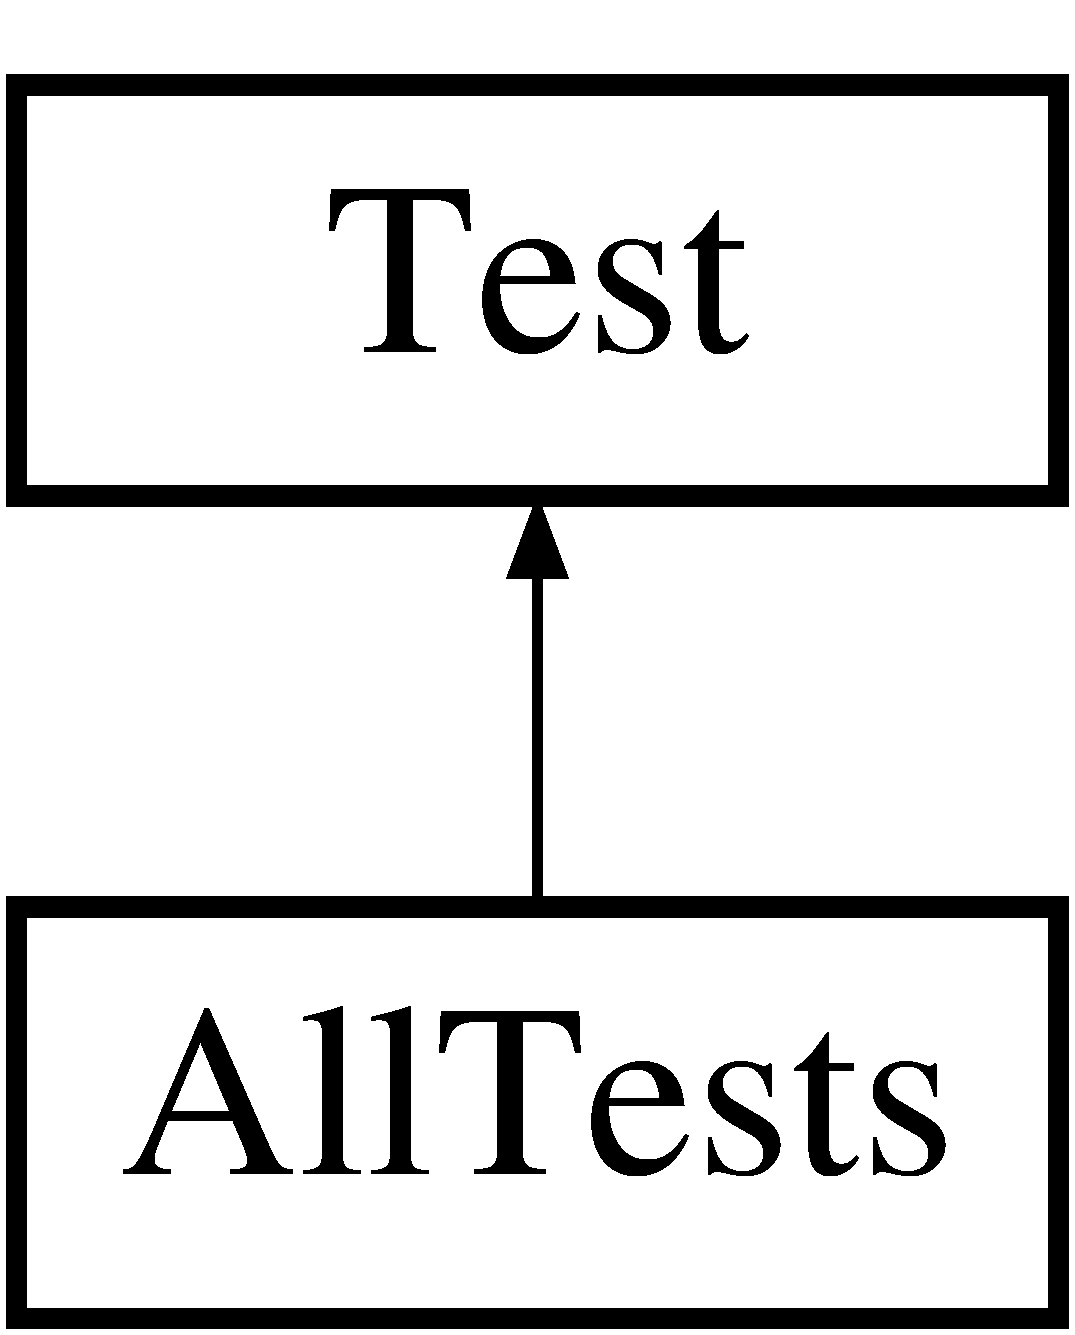
\includegraphics[height=2.000000cm]{class_all_tests}
\end{center}
\end{figure}
\subsection*{Classes}
\begin{DoxyCompactItemize}
\item 
struct \mbox{\hyperlink{struct_all_tests_1_1_vertex_data_test_good}{Vertex\+Data\+Test\+Good}}
\end{DoxyCompactItemize}
\subsection*{Public Attributes}
\begin{DoxyCompactItemize}
\item 
std\+::vector$<$ \mbox{\hyperlink{struct_all_tests_1_1_vertex_data_test_good}{Vertex\+Data\+Test\+Good}} $>$ {\bfseries vertices}
\end{DoxyCompactItemize}
\subsection*{Protected Attributes}
\begin{DoxyCompactItemize}
\item 
\mbox{\Hypertarget{class_all_tests_af766f20e15be66a87c3d5cf40023f5ca}\label{class_all_tests_af766f20e15be66a87c3d5cf40023f5ca}} 
\mbox{\hyperlink{class_window}{Window}} {\bfseries window} = \mbox{\hyperlink{class_window}{Window}}(800, 600, \char`\"{}Test\char`\"{})
\item 
\mbox{\Hypertarget{class_all_tests_a16a47ee1ab2efbc1b02140320e2e8060}\label{class_all_tests_a16a47ee1ab2efbc1b02140320e2e8060}} 
const std\+::string {\bfseries awesomefacetexturepath} = T\+E\+X\+T\+U\+R\+E\+\_\+\+F\+O\+L\+D\+ER + std\+::string(\char`\"{}awesomeface.\+png\char`\"{})
\item 
\mbox{\Hypertarget{class_all_tests_ad397c6216ebfac27d73c41d2695a3a57}\label{class_all_tests_ad397c6216ebfac27d73c41d2695a3a57}} 
\mbox{\hyperlink{classpiolot_1_1_texture}{Texture}} {\bfseries awesome\+Face\+Texture} = \mbox{\hyperlink{classpiolot_1_1_texture}{Texture}}(awesomefacetexturepath)
\item 
\mbox{\Hypertarget{class_all_tests_aa359901bc51c6481aec854caec7b7cc6}\label{class_all_tests_aa359901bc51c6481aec854caec7b7cc6}} 
std\+::string {\bfseries test\+\_\+vert\+\_\+file\+\_\+2} = S\+H\+A\+D\+E\+R\+\_\+\+F\+O\+L\+D\+ER + std\+::string(\char`\"{}good\+\_\+test.\+vert\char`\"{})
\item 
\mbox{\Hypertarget{class_all_tests_a1a8ac7b45dadaaf7008f7b3892b72d9f}\label{class_all_tests_a1a8ac7b45dadaaf7008f7b3892b72d9f}} 
std\+::string {\bfseries test\+\_\+frag\+\_\+file\+\_\+2} = S\+H\+A\+D\+E\+R\+\_\+\+F\+O\+L\+D\+ER + std\+::string(\char`\"{}good\+\_\+test.\+frag\char`\"{})
\item 
\mbox{\Hypertarget{class_all_tests_a7f041c3c700f521110913724c5bf4ad5}\label{class_all_tests_a7f041c3c700f521110913724c5bf4ad5}} 
\mbox{\hyperlink{classpiolot_1_1_g_l_shader}{G\+L\+Shader}} {\bfseries right\+\_\+shader} = \mbox{\hyperlink{classpiolot_1_1_g_l_shader}{G\+L\+Shader}}(test\+\_\+vert\+\_\+file\+\_\+2.\+c\+\_\+str(), test\+\_\+frag\+\_\+file\+\_\+2.\+c\+\_\+str())
\end{DoxyCompactItemize}


\subsection{Member Data Documentation}
\mbox{\Hypertarget{class_all_tests_acf1a6c04a22fe002610646fc4f1a4fbb}\label{class_all_tests_acf1a6c04a22fe002610646fc4f1a4fbb}} 
\index{All\+Tests@{All\+Tests}!vertices@{vertices}}
\index{vertices@{vertices}!All\+Tests@{All\+Tests}}
\subsubsection{\texorpdfstring{vertices}{vertices}}
{\footnotesize\ttfamily std\+::vector$<$\mbox{\hyperlink{struct_all_tests_1_1_vertex_data_test_good}{Vertex\+Data\+Test\+Good}}$>$ All\+Tests\+::vertices}

{\bfseries Initial value\+:}
\begin{DoxyCode}
= \{
        VertexDataTestGood(glm::vec3(0.5f, -0.5f, 0.0f), glm::vec3(1.0f, 0.0f, 0.0f), glm::vec3(1.0f, 0.0f,
       0.0f)),
        VertexDataTestGood(glm::vec3(-0.5f, -0.5f, 0.0f), glm::vec3(0.0f, 1.0f, 0.0f), glm::vec3(0.0f, 0.0f
      , 0.0f)),
        VertexDataTestGood(glm::vec3(0.0f, 0.5f, 0.0f), glm::vec3(0.0f, 0.0f, 1.0f), glm::vec3(0.5f, 1.0f, 
      0.0f))
    \}
\end{DoxyCode}


The documentation for this class was generated from the following file\+:\begin{DoxyCompactItemize}
\item 
C\+:/dev/\+Piolot/\+Engine/All\+Tests.\+h\end{DoxyCompactItemize}

\hypertarget{classpiolot_1_1_asset_manager}{}\section{piolot\+:\+:Asset\+Manager Class Reference}
\label{classpiolot_1_1_asset_manager}\index{piolot\+::\+Asset\+Manager@{piolot\+::\+Asset\+Manager}}


The Singleton class that holds all the data for Shaders, Textures and Objects.  




{\ttfamily \#include $<$Asset\+Manager.\+h$>$}

\subsection*{Public Member Functions}
\begin{DoxyCompactItemize}
\item 
void \mbox{\hyperlink{classpiolot_1_1_asset_manager_ab6e938de7632862bfbe0a673b6c53b21}{Clear\+All\+Data}} ()
\begin{DoxyCompactList}\small\item\em Remove all the data and clear the Asset Manager. \end{DoxyCompactList}\item 
\mbox{\hyperlink{classpiolot_1_1_asset_manager_a49967e4909436ff8ebaeadf08db4ebc7}{$\sim$\+Asset\+Manager}} ()
\begin{DoxyCompactList}\small\item\em Default Constructor. \end{DoxyCompactList}\item 
\mbox{\Hypertarget{classpiolot_1_1_asset_manager_ac56fdedc1bf3b98909856099811fa62f}\label{classpiolot_1_1_asset_manager_ac56fdedc1bf3b98909856099811fa62f}} 
bool \mbox{\hyperlink{classpiolot_1_1_asset_manager_ac56fdedc1bf3b98909856099811fa62f}{Load\+Shaders}} ()
\begin{DoxyCompactList}\small\item\em Loads all the shaders from the Shader Directory. \end{DoxyCompactList}\item 
\mbox{\Hypertarget{classpiolot_1_1_asset_manager_a34593c7f84f33abd929daa8510507881}\label{classpiolot_1_1_asset_manager_a34593c7f84f33abd929daa8510507881}} 
bool \mbox{\hyperlink{classpiolot_1_1_asset_manager_a34593c7f84f33abd929daa8510507881}{Load\+Textures}} ()
\begin{DoxyCompactList}\small\item\em Loads all the Textures from the \mbox{\hyperlink{classpiolot_1_1_texture}{Texture}} Directory. \end{DoxyCompactList}\item 
bool \mbox{\hyperlink{classpiolot_1_1_asset_manager_acc9c8e5aff5c4b93faa151e0efb012f3}{Is\+Texture\+Loaded}} (std\+::string \+\_\+key)
\begin{DoxyCompactList}\small\item\em Returns if the texture, key is loaded. \end{DoxyCompactList}\item 
bool \mbox{\hyperlink{classpiolot_1_1_asset_manager_a120535d011b245328a45a1d85f181cc0}{Is\+Object\+Loaded}} (std\+::string \+\_\+key)
\begin{DoxyCompactList}\small\item\em Returns if the mesh is loaded. \end{DoxyCompactList}\item 
bool \mbox{\hyperlink{classpiolot_1_1_asset_manager_a06b647312e18c2ca212d34211d262783}{Add\+To\+Textures}} (const std\+::string \&\+\_\+name, std\+::shared\+\_\+ptr$<$ \mbox{\hyperlink{classpiolot_1_1_texture}{Texture}} $>$ \+\_\+texture)
\begin{DoxyCompactList}\small\item\em Add a texture to the exisiting map. \end{DoxyCompactList}\item 
bool \mbox{\hyperlink{classpiolot_1_1_asset_manager_abfad75fa1cde6d1ecd77fbdf297a80b0}{Add\+To\+Objects}} (const std\+::string \&\+\_\+name, std\+::shared\+\_\+ptr$<$ \mbox{\hyperlink{classpiolot_1_1_object}{Object}} $>$ \+\_\+object)
\begin{DoxyCompactList}\small\item\em Add an object to the Map. \end{DoxyCompactList}\item 
void \mbox{\hyperlink{classpiolot_1_1_asset_manager_a00d1b6635e14cfdf2a618fff3ad61416}{Gui\+Render}} (bool $\ast$\+\_\+window\+Flag)
\begin{DoxyCompactList}\small\item\em The Im\+G\+UI calls for the Asset Manager. \end{DoxyCompactList}\end{DoxyCompactItemize}
\subsection*{Static Public Member Functions}
\begin{DoxyCompactItemize}
\item 
static \mbox{\hyperlink{classpiolot_1_1_asset_manager}{Asset\+Manager}} \& \mbox{\hyperlink{classpiolot_1_1_asset_manager_a5bcfd6d2719bcada7f5865eb6e39664b}{get\+Instance}} ()
\begin{DoxyCompactList}\small\item\em Returns the instance of the Singleton. \end{DoxyCompactList}\end{DoxyCompactItemize}
\subsection*{Public Attributes}
\begin{DoxyCompactItemize}
\item 
\mbox{\Hypertarget{classpiolot_1_1_asset_manager_ae8db7f8aa294e32d270181e4ba87d2ad}\label{classpiolot_1_1_asset_manager_ae8db7f8aa294e32d270181e4ba87d2ad}} 
std\+::map$<$ std\+::string, std\+::shared\+\_\+ptr$<$ \mbox{\hyperlink{classpiolot_1_1_g_l_shader}{G\+L\+Shader}} $>$ $>$ \mbox{\hyperlink{classpiolot_1_1_asset_manager_ae8db7f8aa294e32d270181e4ba87d2ad}{shaders}}
\begin{DoxyCompactList}\small\item\em A Map of all the shaders that we load. \end{DoxyCompactList}\item 
\mbox{\Hypertarget{classpiolot_1_1_asset_manager_a6d9403a544a3efd67e33b52d6bb2a182}\label{classpiolot_1_1_asset_manager_a6d9403a544a3efd67e33b52d6bb2a182}} 
std\+::map$<$ std\+::string, std\+::shared\+\_\+ptr$<$ \mbox{\hyperlink{classpiolot_1_1_texture}{Texture}} $>$ $>$ \mbox{\hyperlink{classpiolot_1_1_asset_manager_a6d9403a544a3efd67e33b52d6bb2a182}{textures}}
\begin{DoxyCompactList}\small\item\em A Map of all the textures that we load. \end{DoxyCompactList}\item 
\mbox{\Hypertarget{classpiolot_1_1_asset_manager_a5051f83ff594361ac33d94a885afde10}\label{classpiolot_1_1_asset_manager_a5051f83ff594361ac33d94a885afde10}} 
std\+::map$<$ std\+::string, std\+::shared\+\_\+ptr$<$ \mbox{\hyperlink{classpiolot_1_1_object}{Object}} $>$ $>$ \mbox{\hyperlink{classpiolot_1_1_asset_manager_a5051f83ff594361ac33d94a885afde10}{objects}}
\begin{DoxyCompactList}\small\item\em A Map of all the Renderables loaded. \end{DoxyCompactList}\item 
\mbox{\Hypertarget{classpiolot_1_1_asset_manager_a0c7c10a24343176f2de6aeb2ddf1ac0d}\label{classpiolot_1_1_asset_manager_a0c7c10a24343176f2de6aeb2ddf1ac0d}} 
std\+::string \mbox{\hyperlink{classpiolot_1_1_asset_manager_a0c7c10a24343176f2de6aeb2ddf1ac0d}{shader\+Dir}} = S\+H\+A\+D\+E\+R\+\_\+\+F\+O\+L\+D\+ER
\begin{DoxyCompactList}\small\item\em The Shader Directory from where all the shaders are loaded. \end{DoxyCompactList}\item 
\mbox{\Hypertarget{classpiolot_1_1_asset_manager_a001707738b5a8e9da3fd5bfd3557392a}\label{classpiolot_1_1_asset_manager_a001707738b5a8e9da3fd5bfd3557392a}} 
std\+::string \mbox{\hyperlink{classpiolot_1_1_asset_manager_a001707738b5a8e9da3fd5bfd3557392a}{texture\+Dir}} = T\+E\+X\+T\+U\+R\+E\+\_\+\+F\+O\+L\+D\+ER
\begin{DoxyCompactList}\small\item\em The \mbox{\hyperlink{classpiolot_1_1_texture}{Texture}} Directory from where all the Textures are loaded. \end{DoxyCompactList}\end{DoxyCompactItemize}


\subsection{Detailed Description}
The Singleton class that holds all the data for Shaders, Textures and Objects. 

\subsection{Constructor \& Destructor Documentation}
\mbox{\Hypertarget{classpiolot_1_1_asset_manager_a49967e4909436ff8ebaeadf08db4ebc7}\label{classpiolot_1_1_asset_manager_a49967e4909436ff8ebaeadf08db4ebc7}} 
\index{piolot\+::\+Asset\+Manager@{piolot\+::\+Asset\+Manager}!````~Asset\+Manager@{$\sim$\+Asset\+Manager}}
\index{````~Asset\+Manager@{$\sim$\+Asset\+Manager}!piolot\+::\+Asset\+Manager@{piolot\+::\+Asset\+Manager}}
\subsubsection{\texorpdfstring{$\sim$\+Asset\+Manager()}{~AssetManager()}}
{\footnotesize\ttfamily piolot\+::\+Asset\+Manager\+::$\sim$\+Asset\+Manager (\begin{DoxyParamCaption}{ }\end{DoxyParamCaption})\hspace{0.3cm}{\ttfamily [inline]}}



Default Constructor. 

Destructor. Deletes all the Shaders and Textures stored here. 

\subsection{Member Function Documentation}
\mbox{\Hypertarget{classpiolot_1_1_asset_manager_abfad75fa1cde6d1ecd77fbdf297a80b0}\label{classpiolot_1_1_asset_manager_abfad75fa1cde6d1ecd77fbdf297a80b0}} 
\index{piolot\+::\+Asset\+Manager@{piolot\+::\+Asset\+Manager}!Add\+To\+Objects@{Add\+To\+Objects}}
\index{Add\+To\+Objects@{Add\+To\+Objects}!piolot\+::\+Asset\+Manager@{piolot\+::\+Asset\+Manager}}
\subsubsection{\texorpdfstring{Add\+To\+Objects()}{AddToObjects()}}
{\footnotesize\ttfamily bool piolot\+::\+Asset\+Manager\+::\+Add\+To\+Objects (\begin{DoxyParamCaption}\item[{const std\+::string \&}]{\+\_\+name,  }\item[{std\+::shared\+\_\+ptr$<$ \mbox{\hyperlink{classpiolot_1_1_object}{Object}} $>$}]{\+\_\+object }\end{DoxyParamCaption})\hspace{0.3cm}{\ttfamily [inline]}}



Add an object to the Map. 


\begin{DoxyParams}{Parameters}
{\em \+\_\+name} & The Key \\
\hline
{\em \+\_\+object} & The \mbox{\hyperlink{classpiolot_1_1_object}{Object}} \\
\hline
\end{DoxyParams}
\begin{DoxyReturn}{Returns}
If the \mbox{\hyperlink{classpiolot_1_1_object}{Object}} is already loaded, returns false. Else, returns True. 
\end{DoxyReturn}
\mbox{\Hypertarget{classpiolot_1_1_asset_manager_a06b647312e18c2ca212d34211d262783}\label{classpiolot_1_1_asset_manager_a06b647312e18c2ca212d34211d262783}} 
\index{piolot\+::\+Asset\+Manager@{piolot\+::\+Asset\+Manager}!Add\+To\+Textures@{Add\+To\+Textures}}
\index{Add\+To\+Textures@{Add\+To\+Textures}!piolot\+::\+Asset\+Manager@{piolot\+::\+Asset\+Manager}}
\subsubsection{\texorpdfstring{Add\+To\+Textures()}{AddToTextures()}}
{\footnotesize\ttfamily bool piolot\+::\+Asset\+Manager\+::\+Add\+To\+Textures (\begin{DoxyParamCaption}\item[{const std\+::string \&}]{\+\_\+name,  }\item[{std\+::shared\+\_\+ptr$<$ \mbox{\hyperlink{classpiolot_1_1_texture}{Texture}} $>$}]{\+\_\+texture }\end{DoxyParamCaption})\hspace{0.3cm}{\ttfamily [inline]}}



Add a texture to the exisiting map. 


\begin{DoxyParams}{Parameters}
{\em \+\_\+name} & The Key to place the \mbox{\hyperlink{classpiolot_1_1_texture}{Texture}}. \\
\hline
{\em \+\_\+texture} & The \mbox{\hyperlink{classpiolot_1_1_texture}{Texture}} to load and place. \\
\hline
\end{DoxyParams}
\begin{DoxyReturn}{Returns}
Returns true if the \mbox{\hyperlink{classpiolot_1_1_texture}{Texture}} is succesfully loaded. False if something occurs. 
\end{DoxyReturn}
\mbox{\Hypertarget{classpiolot_1_1_asset_manager_ab6e938de7632862bfbe0a673b6c53b21}\label{classpiolot_1_1_asset_manager_ab6e938de7632862bfbe0a673b6c53b21}} 
\index{piolot\+::\+Asset\+Manager@{piolot\+::\+Asset\+Manager}!Clear\+All\+Data@{Clear\+All\+Data}}
\index{Clear\+All\+Data@{Clear\+All\+Data}!piolot\+::\+Asset\+Manager@{piolot\+::\+Asset\+Manager}}
\subsubsection{\texorpdfstring{Clear\+All\+Data()}{ClearAllData()}}
{\footnotesize\ttfamily void piolot\+::\+Asset\+Manager\+::\+Clear\+All\+Data (\begin{DoxyParamCaption}{ }\end{DoxyParamCaption})\hspace{0.3cm}{\ttfamily [inline]}}



Remove all the data and clear the Asset Manager. 

$\ast$for (auto it \+: shaders) \mbox{\Hypertarget{classpiolot_1_1_asset_manager_a5bcfd6d2719bcada7f5865eb6e39664b}\label{classpiolot_1_1_asset_manager_a5bcfd6d2719bcada7f5865eb6e39664b}} 
\index{piolot\+::\+Asset\+Manager@{piolot\+::\+Asset\+Manager}!get\+Instance@{get\+Instance}}
\index{get\+Instance@{get\+Instance}!piolot\+::\+Asset\+Manager@{piolot\+::\+Asset\+Manager}}
\subsubsection{\texorpdfstring{get\+Instance()}{getInstance()}}
{\footnotesize\ttfamily \mbox{\hyperlink{classpiolot_1_1_asset_manager}{Asset\+Manager}} \& piolot\+::\+Asset\+Manager\+::get\+Instance (\begin{DoxyParamCaption}{ }\end{DoxyParamCaption})\hspace{0.3cm}{\ttfamily [inline]}, {\ttfamily [static]}}



Returns the instance of the Singleton. 

\begin{DoxyReturn}{Returns}
The reference to the static object, instance. 
\end{DoxyReturn}
\mbox{\Hypertarget{classpiolot_1_1_asset_manager_a00d1b6635e14cfdf2a618fff3ad61416}\label{classpiolot_1_1_asset_manager_a00d1b6635e14cfdf2a618fff3ad61416}} 
\index{piolot\+::\+Asset\+Manager@{piolot\+::\+Asset\+Manager}!Gui\+Render@{Gui\+Render}}
\index{Gui\+Render@{Gui\+Render}!piolot\+::\+Asset\+Manager@{piolot\+::\+Asset\+Manager}}
\subsubsection{\texorpdfstring{Gui\+Render()}{GuiRender()}}
{\footnotesize\ttfamily void piolot\+::\+Asset\+Manager\+::\+Gui\+Render (\begin{DoxyParamCaption}\item[{bool $\ast$}]{\+\_\+window\+Flag }\end{DoxyParamCaption})\hspace{0.3cm}{\ttfamily [inline]}}



The Im\+G\+UI calls for the Asset Manager. 


\begin{DoxyParams}{Parameters}
{\em \+\_\+window\+Flag} & The \mbox{\hyperlink{class_window}{Window}} is Open Boolean \\
\hline
\end{DoxyParams}
\mbox{\Hypertarget{classpiolot_1_1_asset_manager_a120535d011b245328a45a1d85f181cc0}\label{classpiolot_1_1_asset_manager_a120535d011b245328a45a1d85f181cc0}} 
\index{piolot\+::\+Asset\+Manager@{piolot\+::\+Asset\+Manager}!Is\+Object\+Loaded@{Is\+Object\+Loaded}}
\index{Is\+Object\+Loaded@{Is\+Object\+Loaded}!piolot\+::\+Asset\+Manager@{piolot\+::\+Asset\+Manager}}
\subsubsection{\texorpdfstring{Is\+Object\+Loaded()}{IsObjectLoaded()}}
{\footnotesize\ttfamily bool piolot\+::\+Asset\+Manager\+::\+Is\+Object\+Loaded (\begin{DoxyParamCaption}\item[{std\+::string}]{\+\_\+key }\end{DoxyParamCaption})\hspace{0.3cm}{\ttfamily [inline]}}



Returns if the mesh is loaded. 


\begin{DoxyParams}{Parameters}
{\em \+\_\+key} & Key \\
\hline
\end{DoxyParams}
\begin{DoxyReturn}{Returns}
True if we find the mesh with the key. 
\end{DoxyReturn}
\mbox{\Hypertarget{classpiolot_1_1_asset_manager_acc9c8e5aff5c4b93faa151e0efb012f3}\label{classpiolot_1_1_asset_manager_acc9c8e5aff5c4b93faa151e0efb012f3}} 
\index{piolot\+::\+Asset\+Manager@{piolot\+::\+Asset\+Manager}!Is\+Texture\+Loaded@{Is\+Texture\+Loaded}}
\index{Is\+Texture\+Loaded@{Is\+Texture\+Loaded}!piolot\+::\+Asset\+Manager@{piolot\+::\+Asset\+Manager}}
\subsubsection{\texorpdfstring{Is\+Texture\+Loaded()}{IsTextureLoaded()}}
{\footnotesize\ttfamily bool piolot\+::\+Asset\+Manager\+::\+Is\+Texture\+Loaded (\begin{DoxyParamCaption}\item[{std\+::string}]{\+\_\+key }\end{DoxyParamCaption})\hspace{0.3cm}{\ttfamily [inline]}}



Returns if the texture, key is loaded. 


\begin{DoxyParams}{Parameters}
{\em \+\_\+key} & The string, key to look for in the map. \\
\hline
\end{DoxyParams}
\begin{DoxyReturn}{Returns}
Returns True if we can find the texture in the map. 
\end{DoxyReturn}


The documentation for this class was generated from the following files\+:\begin{DoxyCompactItemize}
\item 
C\+:/dev/\+Piolot/\+Engine/Asset\+Manager.\+h\item 
C\+:/dev/\+Piolot/\+Engine/Asset\+Manager.\+cpp\end{DoxyCompactItemize}

\hypertarget{classpiolot_1_1_bounding_box}{}\section{piolot\+:\+:Bounding\+Box Class Reference}
\label{classpiolot_1_1_bounding_box}\index{piolot\+::\+Bounding\+Box@{piolot\+::\+Bounding\+Box}}


This class is used to create a simple cuboid around the Objects as a Bounding Box.  




{\ttfamily \#include $<$Bounding\+Box.\+h$>$}

\subsection*{Public Member Functions}
\begin{DoxyCompactItemize}
\item 
const glm\+::vec3 \& \mbox{\hyperlink{group___getters_ga1534921bb22645320614b4cf02268906}{Get\+Minimum\+Point}} () const
\item 
const glm\+::vec3 \& \mbox{\hyperlink{group___getters_gafd9222c8fb47c5484c873ace9d66a37d}{Get\+Maximum\+Point}} () const
\item 
unsigned int \mbox{\hyperlink{group___getters_ga57651f343f21133fc6c89c8c5619ed84}{Get\+Vertices\+Size}} () const
\item 
\mbox{\hyperlink{group___getters_ga699e27e8e646be7a0a47f89abb35778d}{Bounding\+Box}} (glm\+::vec3 \+\_\+minimum\+Point=glm\+::vec3(-\/0.\+2f, -\/0.\+2f, -\/0.\+2f), glm\+::vec3 \+\_\+maximum\+Point=glm\+::vec3(0.\+2f, 0.\+2f, 0.\+2f))
\begin{DoxyCompactList}\small\item\em Constructor. \end{DoxyCompactList}\item 
bool \mbox{\hyperlink{group___getters_ga552fcdb461cdc71c5da0fed7b486246d}{Check\+For\+Collision\+With\+Ray}} (const glm\+::mat4 \+\_\+model\+Matrix, const glm\+::vec3 \+\_\+scale, const glm\+::vec3 \+\_\+ray\+Origin, const glm\+::vec3 \+\_\+ray\+Direction, float \&\+\_\+intersection\+Distance) const
\begin{DoxyCompactList}\small\item\em Check if the Bounding Box Collides with the \mbox{\hyperlink{classpiolot_1_1_ray}{Ray}}. \end{DoxyCompactList}\item 
void \mbox{\hyperlink{group___getters_ga3ef9f966674be7fa0448d388b7a3d776}{Render}} (glm\+::vec3 \+\_\+colour)
\begin{DoxyCompactList}\small\item\em Render the Bounding Box. \end{DoxyCompactList}\end{DoxyCompactItemize}
\subsection*{Protected Attributes}
\begin{DoxyCompactItemize}
\item 
glm\+::vec3 \mbox{\hyperlink{classpiolot_1_1_bounding_box_a9e1b1896cdc55746ab9903241c358dc4}{minimum\+Point}}
\begin{DoxyCompactList}\small\item\em The Minimum point of the Cuboid in 3D Space. Typically, the Bottom, Left, -\/Z Point. \end{DoxyCompactList}\item 
glm\+::vec3 \mbox{\hyperlink{classpiolot_1_1_bounding_box_a4b6af7e1b8cb46c8967a8921146097bd}{maximum\+Point}}
\begin{DoxyCompactList}\small\item\em The Maximum point of the Cuboid. Typically, the Right, Top, +Z Point. \end{DoxyCompactList}\item 
std\+::vector$<$ glm\+::vec3 $>$ \mbox{\hyperlink{classpiolot_1_1_bounding_box_ae57572db987c9f1185ad73febc8fbc28}{vertices}}
\begin{DoxyCompactList}\small\item\em The Vertices for the Cuboid. Will be computed based on the Min and Max Points. \end{DoxyCompactList}\item 
unsigned int \mbox{\hyperlink{classpiolot_1_1_bounding_box_ad5ea73dcadf0d25c07cc8ff3761db4e3}{V\+AO}}
\begin{DoxyCompactList}\small\item\em Vertex Array \mbox{\hyperlink{classpiolot_1_1_object}{Object}} ID. Used for Rendering the B\+Box. \end{DoxyCompactList}\item 
unsigned int \mbox{\hyperlink{classpiolot_1_1_bounding_box_a4c8c26e00dff9f14709bc2803b38a0bf}{V\+BO}}
\begin{DoxyCompactList}\small\item\em Vertex Buffer \mbox{\hyperlink{classpiolot_1_1_object}{Object}} ID. Used for Rendering the B\+Box. \end{DoxyCompactList}\end{DoxyCompactItemize}


\subsection{Detailed Description}
This class is used to create a simple cuboid around the Objects as a Bounding Box. 

\subsection{Member Data Documentation}
\mbox{\Hypertarget{classpiolot_1_1_bounding_box_a4b6af7e1b8cb46c8967a8921146097bd}\label{classpiolot_1_1_bounding_box_a4b6af7e1b8cb46c8967a8921146097bd}} 
\index{piolot\+::\+Bounding\+Box@{piolot\+::\+Bounding\+Box}!maximum\+Point@{maximum\+Point}}
\index{maximum\+Point@{maximum\+Point}!piolot\+::\+Bounding\+Box@{piolot\+::\+Bounding\+Box}}
\subsubsection{\texorpdfstring{maximum\+Point}{maximumPoint}}
{\footnotesize\ttfamily glm\+::vec3 piolot\+::\+Bounding\+Box\+::maximum\+Point\hspace{0.3cm}{\ttfamily [protected]}}



The Maximum point of the Cuboid. Typically, the Right, Top, +Z Point. 

\mbox{\Hypertarget{classpiolot_1_1_bounding_box_a9e1b1896cdc55746ab9903241c358dc4}\label{classpiolot_1_1_bounding_box_a9e1b1896cdc55746ab9903241c358dc4}} 
\index{piolot\+::\+Bounding\+Box@{piolot\+::\+Bounding\+Box}!minimum\+Point@{minimum\+Point}}
\index{minimum\+Point@{minimum\+Point}!piolot\+::\+Bounding\+Box@{piolot\+::\+Bounding\+Box}}
\subsubsection{\texorpdfstring{minimum\+Point}{minimumPoint}}
{\footnotesize\ttfamily glm\+::vec3 piolot\+::\+Bounding\+Box\+::minimum\+Point\hspace{0.3cm}{\ttfamily [protected]}}



The Minimum point of the Cuboid in 3D Space. Typically, the Bottom, Left, -\/Z Point. 

\mbox{\Hypertarget{classpiolot_1_1_bounding_box_ad5ea73dcadf0d25c07cc8ff3761db4e3}\label{classpiolot_1_1_bounding_box_ad5ea73dcadf0d25c07cc8ff3761db4e3}} 
\index{piolot\+::\+Bounding\+Box@{piolot\+::\+Bounding\+Box}!V\+AO@{V\+AO}}
\index{V\+AO@{V\+AO}!piolot\+::\+Bounding\+Box@{piolot\+::\+Bounding\+Box}}
\subsubsection{\texorpdfstring{V\+AO}{VAO}}
{\footnotesize\ttfamily unsigned int piolot\+::\+Bounding\+Box\+::\+V\+AO\hspace{0.3cm}{\ttfamily [protected]}}



Vertex Array \mbox{\hyperlink{classpiolot_1_1_object}{Object}} ID. Used for Rendering the B\+Box. 

\mbox{\Hypertarget{classpiolot_1_1_bounding_box_a4c8c26e00dff9f14709bc2803b38a0bf}\label{classpiolot_1_1_bounding_box_a4c8c26e00dff9f14709bc2803b38a0bf}} 
\index{piolot\+::\+Bounding\+Box@{piolot\+::\+Bounding\+Box}!V\+BO@{V\+BO}}
\index{V\+BO@{V\+BO}!piolot\+::\+Bounding\+Box@{piolot\+::\+Bounding\+Box}}
\subsubsection{\texorpdfstring{V\+BO}{VBO}}
{\footnotesize\ttfamily unsigned int piolot\+::\+Bounding\+Box\+::\+V\+BO\hspace{0.3cm}{\ttfamily [protected]}}



Vertex Buffer \mbox{\hyperlink{classpiolot_1_1_object}{Object}} ID. Used for Rendering the B\+Box. 

\mbox{\Hypertarget{classpiolot_1_1_bounding_box_ae57572db987c9f1185ad73febc8fbc28}\label{classpiolot_1_1_bounding_box_ae57572db987c9f1185ad73febc8fbc28}} 
\index{piolot\+::\+Bounding\+Box@{piolot\+::\+Bounding\+Box}!vertices@{vertices}}
\index{vertices@{vertices}!piolot\+::\+Bounding\+Box@{piolot\+::\+Bounding\+Box}}
\subsubsection{\texorpdfstring{vertices}{vertices}}
{\footnotesize\ttfamily std\+::vector$<$glm\+::vec3$>$ piolot\+::\+Bounding\+Box\+::vertices\hspace{0.3cm}{\ttfamily [protected]}}



The Vertices for the Cuboid. Will be computed based on the Min and Max Points. 



The documentation for this class was generated from the following files\+:\begin{DoxyCompactItemize}
\item 
\mbox{\hyperlink{_bounding_box_8h}{Bounding\+Box.\+h}}\item 
\mbox{\hyperlink{_bounding_box_8cpp}{Bounding\+Box.\+cpp}}\end{DoxyCompactItemize}

\hypertarget{classpiolot_1_1_camera}{}\section{piolot\+:\+:Camera Class Reference}
\label{classpiolot_1_1_camera}\index{piolot\+::\+Camera@{piolot\+::\+Camera}}


{\ttfamily \#include $<$Camera.\+h$>$}

\subsection*{Public Types}
\begin{DoxyCompactItemize}
\item 
enum \mbox{\hyperlink{classpiolot_1_1_camera_afba5e0e4539ee7666e8354842c4988e0}{camera\+\_\+movement}} \{ \mbox{\hyperlink{classpiolot_1_1_camera_afba5e0e4539ee7666e8354842c4988e0a0cb80fe1877fddc4afdeb7bb00785842}{forward}}, 
\mbox{\hyperlink{classpiolot_1_1_camera_afba5e0e4539ee7666e8354842c4988e0a54badf21a866512cc17c36e2cf1b4aa6}{back}}, 
\mbox{\hyperlink{classpiolot_1_1_camera_afba5e0e4539ee7666e8354842c4988e0a4f24534e1ab495cce0a63f8e28fda1b9}{rightside}}, 
\mbox{\hyperlink{classpiolot_1_1_camera_afba5e0e4539ee7666e8354842c4988e0a25379d6baed208220bc99d359283c5e8}{leftside}}
 \}
\end{DoxyCompactItemize}
\subsection*{Public Member Functions}
\begin{DoxyCompactItemize}
\item 
std\+::string \& \mbox{\hyperlink{classpiolot_1_1_camera_ae4322f03375c71eae72b7238a1c4ac12}{Get\+Camera\+Name}} ()
\item 
\mbox{\hyperlink{classpiolot_1_1_camera_a7c525f53bc93d1627261d40674e96104}{Camera}} (std\+::string \+\_\+camera\+Name=\char`\"{}default\char`\"{}, glm\+::vec3 \+\_\+position=glm\+::vec3(0, 0, 10), glm\+::vec3 \+\_\+front=glm\+::vec3(0, 0, -\/1), glm\+::vec3 \+\_\+world\+Up=glm\+::vec3(0, 1, 0), \mbox{\hyperlink{namespacepiolot_a8ffac0a73d973fb66879963da5defc90}{Camera\+Type}} \+\_\+type=\mbox{\hyperlink{namespacepiolot_a8ffac0a73d973fb66879963da5defc90a2306e17263193ee4e70fe9756faef528}{perspective}}, float \+\_\+movement\+Speed=\mbox{\hyperlink{namespacepiolot_ad09978d4f33e2559089adbc964c31992}{default\+\_\+camera\+\_\+speed}}, float \+\_\+mouse\+Sensitivity=\mbox{\hyperlink{namespacepiolot_a748a31cf105e50f2a20ccaba5fd374d3}{default\+\_\+camera\+\_\+mouse\+\_\+sensitivity}})
\item 
\mbox{\hyperlink{classpiolot_1_1_camera_a0d693a4be11bfc98a2cb46c4363ed00f}{$\sim$\+Camera}} ()=default
\item 
glm\+::vec3 \& \mbox{\hyperlink{classpiolot_1_1_camera_a9c12125ca134fdf776a296c0fac4a79f}{Get\+Position}} ()
\item 
void \mbox{\hyperlink{classpiolot_1_1_camera_a84ff7b1edc39841dddc485fb9e641bf1}{Set\+Position}} (const glm\+::vec3 \&\+\_\+position)
\item 
const glm\+::vec3 \& \mbox{\hyperlink{classpiolot_1_1_camera_a6a428b0f65c9f2b3b5c5c028a96fb1f7}{Get\+Front}} () const
\item 
void \mbox{\hyperlink{classpiolot_1_1_camera_a6151125f42016135376a60182acb63ef}{Set\+Front}} (const glm\+::vec3 \&\+\_\+front)
\item 
const glm\+::vec3 \& \mbox{\hyperlink{classpiolot_1_1_camera_a9ce10517ad9161abf65b827d1884d785}{Get\+Up}} () const
\item 
const glm\+::vec3 \& \mbox{\hyperlink{classpiolot_1_1_camera_a970d1203b54bb2323f9cbb994366d3b4}{Get\+Right}} () const
\item 
const glm\+::vec3 \& \mbox{\hyperlink{classpiolot_1_1_camera_afe3908486ce13772bf593a666869667a}{Get\+World\+Up}} () const
\item 
float \mbox{\hyperlink{classpiolot_1_1_camera_ad270b37d787605772644f35b844992b0}{Get\+Movement\+Speed}} () const
\item 
void \mbox{\hyperlink{classpiolot_1_1_camera_aaf2988ab05281a6a1404207a76957ad6}{Set\+Movement\+Speed}} (float \+\_\+movement\+Speed)
\item 
float \mbox{\hyperlink{classpiolot_1_1_camera_a4f9b65c8df717b82c3b7193457ce71f0}{Get\+Mouse\+Sensitivity}} () const
\item 
void \mbox{\hyperlink{classpiolot_1_1_camera_ade560e16d6c3775dab0637873e66e762}{Set\+Mouse\+Sensitivity}} (float \+\_\+mouse\+Sensitivity)
\item 
const glm\+::mat4 \& \mbox{\hyperlink{classpiolot_1_1_camera_ad57c30f9e3f381a492b38566eab4b905}{Get\+View\+Matrix}} () const
\item 
void \mbox{\hyperlink{classpiolot_1_1_camera_adf17d4592d4d144ea3deab9d8d5d836d}{Set\+View\+Matrix}} (const glm\+::mat4 \&\+\_\+view\+Matrix)
\item 
void \mbox{\hyperlink{classpiolot_1_1_camera_aa9172dabf1f037963c8f93f7b774cd9e}{Display\+Camera\+Details\+Imgui}} ()
\item 
void \mbox{\hyperlink{classpiolot_1_1_camera_a55a4d1a5773d240f08c766e6566591b3}{Process\+Keyboard}} (\mbox{\hyperlink{classpiolot_1_1_camera_afba5e0e4539ee7666e8354842c4988e0}{camera\+\_\+movement}} \+\_\+direction, float \+\_\+delta\+Time)
\item 
void \mbox{\hyperlink{classpiolot_1_1_camera_ae6e18ad2ee8ca787ffe5fa35a01dd16b}{Process\+Mouse\+Movement}} (float \+\_\+xoffset, float \+\_\+yoffset)
\item 
glm\+::vec3 \mbox{\hyperlink{classpiolot_1_1_camera_a6f2dd8513b5f87e438e2721bd32b22c0}{Get\+Mouse\+Ray\+Direction}} (float \+\_\+mouseX, float \+\_\+mouseY, int \+\_\+window\+Width, int \+\_\+window\+Height, glm\+::mat4 \+\_\+projection\+Matrix)
\item 
void \mbox{\hyperlink{classpiolot_1_1_camera_a3e5675563dc81e8526c012e54cb92c9f}{Update\+Vectors}} ()
\item 
void \mbox{\hyperlink{classpiolot_1_1_camera_a93e6bf77b4c9a6a1402a4866dc2590e9}{Update\+Matrices}} ()
\item 
void \mbox{\hyperlink{classpiolot_1_1_camera_abd25ede2299da256764a59e991a8e25a}{Save\+To\+Stream}} (std\+::ofstream \&\+\_\+out)
\item 
void \mbox{\hyperlink{classpiolot_1_1_camera_acca1f703bec64c28d501760920cf8d57}{Load\+From\+Stream}} (std\+::ifstream \&\+\_\+in)
\end{DoxyCompactItemize}
\subsection*{Protected Attributes}
\begin{DoxyCompactItemize}
\item 
glm\+::vec3 \mbox{\hyperlink{classpiolot_1_1_camera_a4552a5cf81a5a8ed249f632e157947a1}{position}}
\item 
glm\+::vec3 \mbox{\hyperlink{classpiolot_1_1_camera_a2adfedf79a032c96798b7d6e01755b5a}{front}}
\item 
glm\+::vec3 \mbox{\hyperlink{classpiolot_1_1_camera_a31ccd695a741d232fa4592d7713de37e}{up}}
\item 
glm\+::vec3 \mbox{\hyperlink{classpiolot_1_1_camera_a20ee1dceb691bb4eefda7a792a6de7c5}{right}}
\item 
glm\+::vec3 \mbox{\hyperlink{classpiolot_1_1_camera_ae722f7d01f68b23b82feb2adb74b90c2}{world\+Up}}
\item 
float \mbox{\hyperlink{classpiolot_1_1_camera_a92aadc4b56ef9667081ecb52b2d7bc42}{movement\+Speed}} = 0.\+0f
\item 
float \mbox{\hyperlink{classpiolot_1_1_camera_ade10b624b272d00a83fdc969da8755f9}{mouse\+Sensitivity}} = 0.\+0f
\item 
glm\+::mat4 \mbox{\hyperlink{classpiolot_1_1_camera_a8f9352500ba36f03f6a384cc28579a95}{view\+Matrix}}
\item 
std\+::string \mbox{\hyperlink{classpiolot_1_1_camera_acada09a9b00303c10c694c386fa05f87}{camera\+Name}}
\item 
\mbox{\hyperlink{namespacepiolot_a8ffac0a73d973fb66879963da5defc90}{Camera\+Type}} \mbox{\hyperlink{classpiolot_1_1_camera_a782c913d63204fd8e22c17111dc1921f}{type}}
\end{DoxyCompactItemize}


\subsection{Member Enumeration Documentation}
\mbox{\Hypertarget{classpiolot_1_1_camera_afba5e0e4539ee7666e8354842c4988e0}\label{classpiolot_1_1_camera_afba5e0e4539ee7666e8354842c4988e0}} 
\index{piolot\+::\+Camera@{piolot\+::\+Camera}!camera\+\_\+movement@{camera\+\_\+movement}}
\index{camera\+\_\+movement@{camera\+\_\+movement}!piolot\+::\+Camera@{piolot\+::\+Camera}}
\subsubsection{\texorpdfstring{camera\+\_\+movement}{camera\_movement}}
{\footnotesize\ttfamily enum \mbox{\hyperlink{classpiolot_1_1_camera_afba5e0e4539ee7666e8354842c4988e0}{piolot\+::\+Camera\+::camera\+\_\+movement}}}

\begin{DoxyEnumFields}{Enumerator}
\raisebox{\heightof{T}}[0pt][0pt]{\index{forward@{forward}!piolot\+::\+Camera@{piolot\+::\+Camera}}\index{piolot\+::\+Camera@{piolot\+::\+Camera}!forward@{forward}}}\mbox{\Hypertarget{classpiolot_1_1_camera_afba5e0e4539ee7666e8354842c4988e0a0cb80fe1877fddc4afdeb7bb00785842}\label{classpiolot_1_1_camera_afba5e0e4539ee7666e8354842c4988e0a0cb80fe1877fddc4afdeb7bb00785842}} 
forward&\\
\hline

\raisebox{\heightof{T}}[0pt][0pt]{\index{back@{back}!piolot\+::\+Camera@{piolot\+::\+Camera}}\index{piolot\+::\+Camera@{piolot\+::\+Camera}!back@{back}}}\mbox{\Hypertarget{classpiolot_1_1_camera_afba5e0e4539ee7666e8354842c4988e0a54badf21a866512cc17c36e2cf1b4aa6}\label{classpiolot_1_1_camera_afba5e0e4539ee7666e8354842c4988e0a54badf21a866512cc17c36e2cf1b4aa6}} 
back&\\
\hline

\raisebox{\heightof{T}}[0pt][0pt]{\index{rightside@{rightside}!piolot\+::\+Camera@{piolot\+::\+Camera}}\index{piolot\+::\+Camera@{piolot\+::\+Camera}!rightside@{rightside}}}\mbox{\Hypertarget{classpiolot_1_1_camera_afba5e0e4539ee7666e8354842c4988e0a4f24534e1ab495cce0a63f8e28fda1b9}\label{classpiolot_1_1_camera_afba5e0e4539ee7666e8354842c4988e0a4f24534e1ab495cce0a63f8e28fda1b9}} 
rightside&\\
\hline

\raisebox{\heightof{T}}[0pt][0pt]{\index{leftside@{leftside}!piolot\+::\+Camera@{piolot\+::\+Camera}}\index{piolot\+::\+Camera@{piolot\+::\+Camera}!leftside@{leftside}}}\mbox{\Hypertarget{classpiolot_1_1_camera_afba5e0e4539ee7666e8354842c4988e0a25379d6baed208220bc99d359283c5e8}\label{classpiolot_1_1_camera_afba5e0e4539ee7666e8354842c4988e0a25379d6baed208220bc99d359283c5e8}} 
leftside&\\
\hline

\end{DoxyEnumFields}


\subsection{Constructor \& Destructor Documentation}
\mbox{\Hypertarget{classpiolot_1_1_camera_a7c525f53bc93d1627261d40674e96104}\label{classpiolot_1_1_camera_a7c525f53bc93d1627261d40674e96104}} 
\index{piolot\+::\+Camera@{piolot\+::\+Camera}!Camera@{Camera}}
\index{Camera@{Camera}!piolot\+::\+Camera@{piolot\+::\+Camera}}
\subsubsection{\texorpdfstring{Camera()}{Camera()}}
{\footnotesize\ttfamily piolot\+::\+Camera\+::\+Camera (\begin{DoxyParamCaption}\item[{std\+::string}]{\+\_\+camera\+Name = {\ttfamily \char`\"{}default\char`\"{}},  }\item[{glm\+::vec3}]{\+\_\+position = {\ttfamily glm\+:\+:vec3(0,~0,~10)},  }\item[{glm\+::vec3}]{\+\_\+front = {\ttfamily glm\+:\+:vec3(0,~0,~-\/1)},  }\item[{glm\+::vec3}]{\+\_\+world\+Up = {\ttfamily glm\+:\+:vec3(0,~1,~0)},  }\item[{\mbox{\hyperlink{namespacepiolot_a8ffac0a73d973fb66879963da5defc90}{Camera\+Type}}}]{\+\_\+type = {\ttfamily \mbox{\hyperlink{namespacepiolot_a8ffac0a73d973fb66879963da5defc90a2306e17263193ee4e70fe9756faef528}{perspective}}},  }\item[{float}]{\+\_\+movement\+Speed = {\ttfamily \mbox{\hyperlink{namespacepiolot_ad09978d4f33e2559089adbc964c31992}{default\+\_\+camera\+\_\+speed}}},  }\item[{float}]{\+\_\+mouse\+Sensitivity = {\ttfamily \mbox{\hyperlink{namespacepiolot_a748a31cf105e50f2a20ccaba5fd374d3}{default\+\_\+camera\+\_\+mouse\+\_\+sensitivity}}} }\end{DoxyParamCaption})\hspace{0.3cm}{\ttfamily [inline]}}

\mbox{\Hypertarget{classpiolot_1_1_camera_a0d693a4be11bfc98a2cb46c4363ed00f}\label{classpiolot_1_1_camera_a0d693a4be11bfc98a2cb46c4363ed00f}} 
\index{piolot\+::\+Camera@{piolot\+::\+Camera}!````~Camera@{$\sim$\+Camera}}
\index{````~Camera@{$\sim$\+Camera}!piolot\+::\+Camera@{piolot\+::\+Camera}}
\subsubsection{\texorpdfstring{$\sim$\+Camera()}{~Camera()}}
{\footnotesize\ttfamily piolot\+::\+Camera\+::$\sim$\+Camera (\begin{DoxyParamCaption}{ }\end{DoxyParamCaption})\hspace{0.3cm}{\ttfamily [default]}}



\subsection{Member Function Documentation}
\mbox{\Hypertarget{classpiolot_1_1_camera_aa9172dabf1f037963c8f93f7b774cd9e}\label{classpiolot_1_1_camera_aa9172dabf1f037963c8f93f7b774cd9e}} 
\index{piolot\+::\+Camera@{piolot\+::\+Camera}!Display\+Camera\+Details\+Imgui@{Display\+Camera\+Details\+Imgui}}
\index{Display\+Camera\+Details\+Imgui@{Display\+Camera\+Details\+Imgui}!piolot\+::\+Camera@{piolot\+::\+Camera}}
\subsubsection{\texorpdfstring{Display\+Camera\+Details\+Imgui()}{DisplayCameraDetailsImgui()}}
{\footnotesize\ttfamily void piolot\+::\+Camera\+::\+Display\+Camera\+Details\+Imgui (\begin{DoxyParamCaption}{ }\end{DoxyParamCaption})}

\mbox{\Hypertarget{classpiolot_1_1_camera_ae4322f03375c71eae72b7238a1c4ac12}\label{classpiolot_1_1_camera_ae4322f03375c71eae72b7238a1c4ac12}} 
\index{piolot\+::\+Camera@{piolot\+::\+Camera}!Get\+Camera\+Name@{Get\+Camera\+Name}}
\index{Get\+Camera\+Name@{Get\+Camera\+Name}!piolot\+::\+Camera@{piolot\+::\+Camera}}
\subsubsection{\texorpdfstring{Get\+Camera\+Name()}{GetCameraName()}}
{\footnotesize\ttfamily std\+::string\& piolot\+::\+Camera\+::\+Get\+Camera\+Name (\begin{DoxyParamCaption}{ }\end{DoxyParamCaption})\hspace{0.3cm}{\ttfamily [inline]}}

\mbox{\Hypertarget{classpiolot_1_1_camera_a6a428b0f65c9f2b3b5c5c028a96fb1f7}\label{classpiolot_1_1_camera_a6a428b0f65c9f2b3b5c5c028a96fb1f7}} 
\index{piolot\+::\+Camera@{piolot\+::\+Camera}!Get\+Front@{Get\+Front}}
\index{Get\+Front@{Get\+Front}!piolot\+::\+Camera@{piolot\+::\+Camera}}
\subsubsection{\texorpdfstring{Get\+Front()}{GetFront()}}
{\footnotesize\ttfamily const glm\+::vec3\& piolot\+::\+Camera\+::\+Get\+Front (\begin{DoxyParamCaption}{ }\end{DoxyParamCaption}) const\hspace{0.3cm}{\ttfamily [inline]}}

\mbox{\Hypertarget{classpiolot_1_1_camera_a6f2dd8513b5f87e438e2721bd32b22c0}\label{classpiolot_1_1_camera_a6f2dd8513b5f87e438e2721bd32b22c0}} 
\index{piolot\+::\+Camera@{piolot\+::\+Camera}!Get\+Mouse\+Ray\+Direction@{Get\+Mouse\+Ray\+Direction}}
\index{Get\+Mouse\+Ray\+Direction@{Get\+Mouse\+Ray\+Direction}!piolot\+::\+Camera@{piolot\+::\+Camera}}
\subsubsection{\texorpdfstring{Get\+Mouse\+Ray\+Direction()}{GetMouseRayDirection()}}
{\footnotesize\ttfamily glm\+::vec3 piolot\+::\+Camera\+::\+Get\+Mouse\+Ray\+Direction (\begin{DoxyParamCaption}\item[{float}]{\+\_\+mouseX,  }\item[{float}]{\+\_\+mouseY,  }\item[{int}]{\+\_\+window\+Width,  }\item[{int}]{\+\_\+window\+Height,  }\item[{glm\+::mat4}]{\+\_\+projection\+Matrix }\end{DoxyParamCaption})}

\mbox{\Hypertarget{classpiolot_1_1_camera_a4f9b65c8df717b82c3b7193457ce71f0}\label{classpiolot_1_1_camera_a4f9b65c8df717b82c3b7193457ce71f0}} 
\index{piolot\+::\+Camera@{piolot\+::\+Camera}!Get\+Mouse\+Sensitivity@{Get\+Mouse\+Sensitivity}}
\index{Get\+Mouse\+Sensitivity@{Get\+Mouse\+Sensitivity}!piolot\+::\+Camera@{piolot\+::\+Camera}}
\subsubsection{\texorpdfstring{Get\+Mouse\+Sensitivity()}{GetMouseSensitivity()}}
{\footnotesize\ttfamily float piolot\+::\+Camera\+::\+Get\+Mouse\+Sensitivity (\begin{DoxyParamCaption}{ }\end{DoxyParamCaption}) const\hspace{0.3cm}{\ttfamily [inline]}}

\mbox{\Hypertarget{classpiolot_1_1_camera_ad270b37d787605772644f35b844992b0}\label{classpiolot_1_1_camera_ad270b37d787605772644f35b844992b0}} 
\index{piolot\+::\+Camera@{piolot\+::\+Camera}!Get\+Movement\+Speed@{Get\+Movement\+Speed}}
\index{Get\+Movement\+Speed@{Get\+Movement\+Speed}!piolot\+::\+Camera@{piolot\+::\+Camera}}
\subsubsection{\texorpdfstring{Get\+Movement\+Speed()}{GetMovementSpeed()}}
{\footnotesize\ttfamily float piolot\+::\+Camera\+::\+Get\+Movement\+Speed (\begin{DoxyParamCaption}{ }\end{DoxyParamCaption}) const\hspace{0.3cm}{\ttfamily [inline]}}

\mbox{\Hypertarget{classpiolot_1_1_camera_a9c12125ca134fdf776a296c0fac4a79f}\label{classpiolot_1_1_camera_a9c12125ca134fdf776a296c0fac4a79f}} 
\index{piolot\+::\+Camera@{piolot\+::\+Camera}!Get\+Position@{Get\+Position}}
\index{Get\+Position@{Get\+Position}!piolot\+::\+Camera@{piolot\+::\+Camera}}
\subsubsection{\texorpdfstring{Get\+Position()}{GetPosition()}}
{\footnotesize\ttfamily glm\+::vec3\& piolot\+::\+Camera\+::\+Get\+Position (\begin{DoxyParamCaption}{ }\end{DoxyParamCaption})\hspace{0.3cm}{\ttfamily [inline]}}

\mbox{\Hypertarget{classpiolot_1_1_camera_a970d1203b54bb2323f9cbb994366d3b4}\label{classpiolot_1_1_camera_a970d1203b54bb2323f9cbb994366d3b4}} 
\index{piolot\+::\+Camera@{piolot\+::\+Camera}!Get\+Right@{Get\+Right}}
\index{Get\+Right@{Get\+Right}!piolot\+::\+Camera@{piolot\+::\+Camera}}
\subsubsection{\texorpdfstring{Get\+Right()}{GetRight()}}
{\footnotesize\ttfamily const glm\+::vec3\& piolot\+::\+Camera\+::\+Get\+Right (\begin{DoxyParamCaption}{ }\end{DoxyParamCaption}) const\hspace{0.3cm}{\ttfamily [inline]}}

\mbox{\Hypertarget{classpiolot_1_1_camera_a9ce10517ad9161abf65b827d1884d785}\label{classpiolot_1_1_camera_a9ce10517ad9161abf65b827d1884d785}} 
\index{piolot\+::\+Camera@{piolot\+::\+Camera}!Get\+Up@{Get\+Up}}
\index{Get\+Up@{Get\+Up}!piolot\+::\+Camera@{piolot\+::\+Camera}}
\subsubsection{\texorpdfstring{Get\+Up()}{GetUp()}}
{\footnotesize\ttfamily const glm\+::vec3\& piolot\+::\+Camera\+::\+Get\+Up (\begin{DoxyParamCaption}{ }\end{DoxyParamCaption}) const\hspace{0.3cm}{\ttfamily [inline]}}

\mbox{\Hypertarget{classpiolot_1_1_camera_ad57c30f9e3f381a492b38566eab4b905}\label{classpiolot_1_1_camera_ad57c30f9e3f381a492b38566eab4b905}} 
\index{piolot\+::\+Camera@{piolot\+::\+Camera}!Get\+View\+Matrix@{Get\+View\+Matrix}}
\index{Get\+View\+Matrix@{Get\+View\+Matrix}!piolot\+::\+Camera@{piolot\+::\+Camera}}
\subsubsection{\texorpdfstring{Get\+View\+Matrix()}{GetViewMatrix()}}
{\footnotesize\ttfamily const glm\+::mat4\& piolot\+::\+Camera\+::\+Get\+View\+Matrix (\begin{DoxyParamCaption}{ }\end{DoxyParamCaption}) const\hspace{0.3cm}{\ttfamily [inline]}}

\mbox{\Hypertarget{classpiolot_1_1_camera_afe3908486ce13772bf593a666869667a}\label{classpiolot_1_1_camera_afe3908486ce13772bf593a666869667a}} 
\index{piolot\+::\+Camera@{piolot\+::\+Camera}!Get\+World\+Up@{Get\+World\+Up}}
\index{Get\+World\+Up@{Get\+World\+Up}!piolot\+::\+Camera@{piolot\+::\+Camera}}
\subsubsection{\texorpdfstring{Get\+World\+Up()}{GetWorldUp()}}
{\footnotesize\ttfamily const glm\+::vec3\& piolot\+::\+Camera\+::\+Get\+World\+Up (\begin{DoxyParamCaption}{ }\end{DoxyParamCaption}) const\hspace{0.3cm}{\ttfamily [inline]}}

\mbox{\Hypertarget{classpiolot_1_1_camera_acca1f703bec64c28d501760920cf8d57}\label{classpiolot_1_1_camera_acca1f703bec64c28d501760920cf8d57}} 
\index{piolot\+::\+Camera@{piolot\+::\+Camera}!Load\+From\+Stream@{Load\+From\+Stream}}
\index{Load\+From\+Stream@{Load\+From\+Stream}!piolot\+::\+Camera@{piolot\+::\+Camera}}
\subsubsection{\texorpdfstring{Load\+From\+Stream()}{LoadFromStream()}}
{\footnotesize\ttfamily void piolot\+::\+Camera\+::\+Load\+From\+Stream (\begin{DoxyParamCaption}\item[{std\+::ifstream \&}]{\+\_\+in }\end{DoxyParamCaption})}

\mbox{\Hypertarget{classpiolot_1_1_camera_a55a4d1a5773d240f08c766e6566591b3}\label{classpiolot_1_1_camera_a55a4d1a5773d240f08c766e6566591b3}} 
\index{piolot\+::\+Camera@{piolot\+::\+Camera}!Process\+Keyboard@{Process\+Keyboard}}
\index{Process\+Keyboard@{Process\+Keyboard}!piolot\+::\+Camera@{piolot\+::\+Camera}}
\subsubsection{\texorpdfstring{Process\+Keyboard()}{ProcessKeyboard()}}
{\footnotesize\ttfamily void piolot\+::\+Camera\+::\+Process\+Keyboard (\begin{DoxyParamCaption}\item[{\mbox{\hyperlink{classpiolot_1_1_camera_afba5e0e4539ee7666e8354842c4988e0}{camera\+\_\+movement}}}]{\+\_\+direction,  }\item[{float}]{\+\_\+delta\+Time }\end{DoxyParamCaption})}

\mbox{\Hypertarget{classpiolot_1_1_camera_ae6e18ad2ee8ca787ffe5fa35a01dd16b}\label{classpiolot_1_1_camera_ae6e18ad2ee8ca787ffe5fa35a01dd16b}} 
\index{piolot\+::\+Camera@{piolot\+::\+Camera}!Process\+Mouse\+Movement@{Process\+Mouse\+Movement}}
\index{Process\+Mouse\+Movement@{Process\+Mouse\+Movement}!piolot\+::\+Camera@{piolot\+::\+Camera}}
\subsubsection{\texorpdfstring{Process\+Mouse\+Movement()}{ProcessMouseMovement()}}
{\footnotesize\ttfamily void piolot\+::\+Camera\+::\+Process\+Mouse\+Movement (\begin{DoxyParamCaption}\item[{float}]{\+\_\+xoffset,  }\item[{float}]{\+\_\+yoffset }\end{DoxyParamCaption})}

\mbox{\Hypertarget{classpiolot_1_1_camera_abd25ede2299da256764a59e991a8e25a}\label{classpiolot_1_1_camera_abd25ede2299da256764a59e991a8e25a}} 
\index{piolot\+::\+Camera@{piolot\+::\+Camera}!Save\+To\+Stream@{Save\+To\+Stream}}
\index{Save\+To\+Stream@{Save\+To\+Stream}!piolot\+::\+Camera@{piolot\+::\+Camera}}
\subsubsection{\texorpdfstring{Save\+To\+Stream()}{SaveToStream()}}
{\footnotesize\ttfamily void piolot\+::\+Camera\+::\+Save\+To\+Stream (\begin{DoxyParamCaption}\item[{std\+::ofstream \&}]{\+\_\+out }\end{DoxyParamCaption})}

\mbox{\Hypertarget{classpiolot_1_1_camera_a6151125f42016135376a60182acb63ef}\label{classpiolot_1_1_camera_a6151125f42016135376a60182acb63ef}} 
\index{piolot\+::\+Camera@{piolot\+::\+Camera}!Set\+Front@{Set\+Front}}
\index{Set\+Front@{Set\+Front}!piolot\+::\+Camera@{piolot\+::\+Camera}}
\subsubsection{\texorpdfstring{Set\+Front()}{SetFront()}}
{\footnotesize\ttfamily void piolot\+::\+Camera\+::\+Set\+Front (\begin{DoxyParamCaption}\item[{const glm\+::vec3 \&}]{\+\_\+front }\end{DoxyParamCaption})\hspace{0.3cm}{\ttfamily [inline]}}

\mbox{\Hypertarget{classpiolot_1_1_camera_ade560e16d6c3775dab0637873e66e762}\label{classpiolot_1_1_camera_ade560e16d6c3775dab0637873e66e762}} 
\index{piolot\+::\+Camera@{piolot\+::\+Camera}!Set\+Mouse\+Sensitivity@{Set\+Mouse\+Sensitivity}}
\index{Set\+Mouse\+Sensitivity@{Set\+Mouse\+Sensitivity}!piolot\+::\+Camera@{piolot\+::\+Camera}}
\subsubsection{\texorpdfstring{Set\+Mouse\+Sensitivity()}{SetMouseSensitivity()}}
{\footnotesize\ttfamily void piolot\+::\+Camera\+::\+Set\+Mouse\+Sensitivity (\begin{DoxyParamCaption}\item[{float}]{\+\_\+mouse\+Sensitivity }\end{DoxyParamCaption})\hspace{0.3cm}{\ttfamily [inline]}}

\mbox{\Hypertarget{classpiolot_1_1_camera_aaf2988ab05281a6a1404207a76957ad6}\label{classpiolot_1_1_camera_aaf2988ab05281a6a1404207a76957ad6}} 
\index{piolot\+::\+Camera@{piolot\+::\+Camera}!Set\+Movement\+Speed@{Set\+Movement\+Speed}}
\index{Set\+Movement\+Speed@{Set\+Movement\+Speed}!piolot\+::\+Camera@{piolot\+::\+Camera}}
\subsubsection{\texorpdfstring{Set\+Movement\+Speed()}{SetMovementSpeed()}}
{\footnotesize\ttfamily void piolot\+::\+Camera\+::\+Set\+Movement\+Speed (\begin{DoxyParamCaption}\item[{float}]{\+\_\+movement\+Speed }\end{DoxyParamCaption})\hspace{0.3cm}{\ttfamily [inline]}}

\mbox{\Hypertarget{classpiolot_1_1_camera_a84ff7b1edc39841dddc485fb9e641bf1}\label{classpiolot_1_1_camera_a84ff7b1edc39841dddc485fb9e641bf1}} 
\index{piolot\+::\+Camera@{piolot\+::\+Camera}!Set\+Position@{Set\+Position}}
\index{Set\+Position@{Set\+Position}!piolot\+::\+Camera@{piolot\+::\+Camera}}
\subsubsection{\texorpdfstring{Set\+Position()}{SetPosition()}}
{\footnotesize\ttfamily void piolot\+::\+Camera\+::\+Set\+Position (\begin{DoxyParamCaption}\item[{const glm\+::vec3 \&}]{\+\_\+position }\end{DoxyParamCaption})\hspace{0.3cm}{\ttfamily [inline]}}

\mbox{\Hypertarget{classpiolot_1_1_camera_adf17d4592d4d144ea3deab9d8d5d836d}\label{classpiolot_1_1_camera_adf17d4592d4d144ea3deab9d8d5d836d}} 
\index{piolot\+::\+Camera@{piolot\+::\+Camera}!Set\+View\+Matrix@{Set\+View\+Matrix}}
\index{Set\+View\+Matrix@{Set\+View\+Matrix}!piolot\+::\+Camera@{piolot\+::\+Camera}}
\subsubsection{\texorpdfstring{Set\+View\+Matrix()}{SetViewMatrix()}}
{\footnotesize\ttfamily void piolot\+::\+Camera\+::\+Set\+View\+Matrix (\begin{DoxyParamCaption}\item[{const glm\+::mat4 \&}]{\+\_\+view\+Matrix }\end{DoxyParamCaption})\hspace{0.3cm}{\ttfamily [inline]}}

\mbox{\Hypertarget{classpiolot_1_1_camera_a93e6bf77b4c9a6a1402a4866dc2590e9}\label{classpiolot_1_1_camera_a93e6bf77b4c9a6a1402a4866dc2590e9}} 
\index{piolot\+::\+Camera@{piolot\+::\+Camera}!Update\+Matrices@{Update\+Matrices}}
\index{Update\+Matrices@{Update\+Matrices}!piolot\+::\+Camera@{piolot\+::\+Camera}}
\subsubsection{\texorpdfstring{Update\+Matrices()}{UpdateMatrices()}}
{\footnotesize\ttfamily void piolot\+::\+Camera\+::\+Update\+Matrices (\begin{DoxyParamCaption}{ }\end{DoxyParamCaption})}

\mbox{\Hypertarget{classpiolot_1_1_camera_a3e5675563dc81e8526c012e54cb92c9f}\label{classpiolot_1_1_camera_a3e5675563dc81e8526c012e54cb92c9f}} 
\index{piolot\+::\+Camera@{piolot\+::\+Camera}!Update\+Vectors@{Update\+Vectors}}
\index{Update\+Vectors@{Update\+Vectors}!piolot\+::\+Camera@{piolot\+::\+Camera}}
\subsubsection{\texorpdfstring{Update\+Vectors()}{UpdateVectors()}}
{\footnotesize\ttfamily void piolot\+::\+Camera\+::\+Update\+Vectors (\begin{DoxyParamCaption}{ }\end{DoxyParamCaption})}



\subsection{Member Data Documentation}
\mbox{\Hypertarget{classpiolot_1_1_camera_acada09a9b00303c10c694c386fa05f87}\label{classpiolot_1_1_camera_acada09a9b00303c10c694c386fa05f87}} 
\index{piolot\+::\+Camera@{piolot\+::\+Camera}!camera\+Name@{camera\+Name}}
\index{camera\+Name@{camera\+Name}!piolot\+::\+Camera@{piolot\+::\+Camera}}
\subsubsection{\texorpdfstring{camera\+Name}{cameraName}}
{\footnotesize\ttfamily std\+::string piolot\+::\+Camera\+::camera\+Name\hspace{0.3cm}{\ttfamily [protected]}}

\mbox{\Hypertarget{classpiolot_1_1_camera_a2adfedf79a032c96798b7d6e01755b5a}\label{classpiolot_1_1_camera_a2adfedf79a032c96798b7d6e01755b5a}} 
\index{piolot\+::\+Camera@{piolot\+::\+Camera}!front@{front}}
\index{front@{front}!piolot\+::\+Camera@{piolot\+::\+Camera}}
\subsubsection{\texorpdfstring{front}{front}}
{\footnotesize\ttfamily glm\+::vec3 piolot\+::\+Camera\+::front\hspace{0.3cm}{\ttfamily [protected]}}

\mbox{\Hypertarget{classpiolot_1_1_camera_ade10b624b272d00a83fdc969da8755f9}\label{classpiolot_1_1_camera_ade10b624b272d00a83fdc969da8755f9}} 
\index{piolot\+::\+Camera@{piolot\+::\+Camera}!mouse\+Sensitivity@{mouse\+Sensitivity}}
\index{mouse\+Sensitivity@{mouse\+Sensitivity}!piolot\+::\+Camera@{piolot\+::\+Camera}}
\subsubsection{\texorpdfstring{mouse\+Sensitivity}{mouseSensitivity}}
{\footnotesize\ttfamily float piolot\+::\+Camera\+::mouse\+Sensitivity = 0.\+0f\hspace{0.3cm}{\ttfamily [protected]}}

\mbox{\Hypertarget{classpiolot_1_1_camera_a92aadc4b56ef9667081ecb52b2d7bc42}\label{classpiolot_1_1_camera_a92aadc4b56ef9667081ecb52b2d7bc42}} 
\index{piolot\+::\+Camera@{piolot\+::\+Camera}!movement\+Speed@{movement\+Speed}}
\index{movement\+Speed@{movement\+Speed}!piolot\+::\+Camera@{piolot\+::\+Camera}}
\subsubsection{\texorpdfstring{movement\+Speed}{movementSpeed}}
{\footnotesize\ttfamily float piolot\+::\+Camera\+::movement\+Speed = 0.\+0f\hspace{0.3cm}{\ttfamily [protected]}}

\mbox{\Hypertarget{classpiolot_1_1_camera_a4552a5cf81a5a8ed249f632e157947a1}\label{classpiolot_1_1_camera_a4552a5cf81a5a8ed249f632e157947a1}} 
\index{piolot\+::\+Camera@{piolot\+::\+Camera}!position@{position}}
\index{position@{position}!piolot\+::\+Camera@{piolot\+::\+Camera}}
\subsubsection{\texorpdfstring{position}{position}}
{\footnotesize\ttfamily glm\+::vec3 piolot\+::\+Camera\+::position\hspace{0.3cm}{\ttfamily [protected]}}

\mbox{\Hypertarget{classpiolot_1_1_camera_a20ee1dceb691bb4eefda7a792a6de7c5}\label{classpiolot_1_1_camera_a20ee1dceb691bb4eefda7a792a6de7c5}} 
\index{piolot\+::\+Camera@{piolot\+::\+Camera}!right@{right}}
\index{right@{right}!piolot\+::\+Camera@{piolot\+::\+Camera}}
\subsubsection{\texorpdfstring{right}{right}}
{\footnotesize\ttfamily glm\+::vec3 piolot\+::\+Camera\+::right\hspace{0.3cm}{\ttfamily [protected]}}

\mbox{\Hypertarget{classpiolot_1_1_camera_a782c913d63204fd8e22c17111dc1921f}\label{classpiolot_1_1_camera_a782c913d63204fd8e22c17111dc1921f}} 
\index{piolot\+::\+Camera@{piolot\+::\+Camera}!type@{type}}
\index{type@{type}!piolot\+::\+Camera@{piolot\+::\+Camera}}
\subsubsection{\texorpdfstring{type}{type}}
{\footnotesize\ttfamily \mbox{\hyperlink{namespacepiolot_a8ffac0a73d973fb66879963da5defc90}{Camera\+Type}} piolot\+::\+Camera\+::type\hspace{0.3cm}{\ttfamily [protected]}}

\mbox{\Hypertarget{classpiolot_1_1_camera_a31ccd695a741d232fa4592d7713de37e}\label{classpiolot_1_1_camera_a31ccd695a741d232fa4592d7713de37e}} 
\index{piolot\+::\+Camera@{piolot\+::\+Camera}!up@{up}}
\index{up@{up}!piolot\+::\+Camera@{piolot\+::\+Camera}}
\subsubsection{\texorpdfstring{up}{up}}
{\footnotesize\ttfamily glm\+::vec3 piolot\+::\+Camera\+::up\hspace{0.3cm}{\ttfamily [protected]}}

\mbox{\Hypertarget{classpiolot_1_1_camera_a8f9352500ba36f03f6a384cc28579a95}\label{classpiolot_1_1_camera_a8f9352500ba36f03f6a384cc28579a95}} 
\index{piolot\+::\+Camera@{piolot\+::\+Camera}!view\+Matrix@{view\+Matrix}}
\index{view\+Matrix@{view\+Matrix}!piolot\+::\+Camera@{piolot\+::\+Camera}}
\subsubsection{\texorpdfstring{view\+Matrix}{viewMatrix}}
{\footnotesize\ttfamily glm\+::mat4 piolot\+::\+Camera\+::view\+Matrix\hspace{0.3cm}{\ttfamily [protected]}}

\mbox{\Hypertarget{classpiolot_1_1_camera_ae722f7d01f68b23b82feb2adb74b90c2}\label{classpiolot_1_1_camera_ae722f7d01f68b23b82feb2adb74b90c2}} 
\index{piolot\+::\+Camera@{piolot\+::\+Camera}!world\+Up@{world\+Up}}
\index{world\+Up@{world\+Up}!piolot\+::\+Camera@{piolot\+::\+Camera}}
\subsubsection{\texorpdfstring{world\+Up}{worldUp}}
{\footnotesize\ttfamily glm\+::vec3 piolot\+::\+Camera\+::world\+Up\hspace{0.3cm}{\ttfamily [protected]}}



The documentation for this class was generated from the following files\+:\begin{DoxyCompactItemize}
\item 
\mbox{\hyperlink{_camera_8h}{Camera.\+h}}\item 
\mbox{\hyperlink{_camera_8cpp}{Camera.\+cpp}}\end{DoxyCompactItemize}

\hypertarget{structpiolot_1_1_camera_saving_to_stream}{}\section{piolot\+:\+:Camera\+Saving\+To\+Stream Struct Reference}
\label{structpiolot_1_1_camera_saving_to_stream}\index{piolot\+::\+Camera\+Saving\+To\+Stream@{piolot\+::\+Camera\+Saving\+To\+Stream}}
\subsection*{Public Attributes}
\begin{DoxyCompactItemize}
\item 
\mbox{\Hypertarget{structpiolot_1_1_camera_saving_to_stream_a04a032f3c0e8cd93881ce17213bbf4bd}\label{structpiolot_1_1_camera_saving_to_stream_a04a032f3c0e8cd93881ce17213bbf4bd}} 
glm\+::vec3 {\bfseries position}
\item 
\mbox{\Hypertarget{structpiolot_1_1_camera_saving_to_stream_abe0eb65d9c73092e1568f84db1a2aee5}\label{structpiolot_1_1_camera_saving_to_stream_abe0eb65d9c73092e1568f84db1a2aee5}} 
glm\+::vec3 {\bfseries front}
\item 
\mbox{\Hypertarget{structpiolot_1_1_camera_saving_to_stream_a43f2e1bbaaf6bc3b5ccebbe413b25971}\label{structpiolot_1_1_camera_saving_to_stream_a43f2e1bbaaf6bc3b5ccebbe413b25971}} 
glm\+::vec3 {\bfseries up}
\item 
\mbox{\Hypertarget{structpiolot_1_1_camera_saving_to_stream_a7fcc0104c11130ecab709a89768c502c}\label{structpiolot_1_1_camera_saving_to_stream_a7fcc0104c11130ecab709a89768c502c}} 
glm\+::vec3 {\bfseries right}
\item 
\mbox{\Hypertarget{structpiolot_1_1_camera_saving_to_stream_acafc5157ece98eb00acf67acb5b66c88}\label{structpiolot_1_1_camera_saving_to_stream_acafc5157ece98eb00acf67acb5b66c88}} 
glm\+::vec3 {\bfseries world\+Up}
\item 
\mbox{\Hypertarget{structpiolot_1_1_camera_saving_to_stream_ad61906be234d7d739202791be26a2da0}\label{structpiolot_1_1_camera_saving_to_stream_ad61906be234d7d739202791be26a2da0}} 
float {\bfseries movement\+Speed} = 0.\+0f
\item 
\mbox{\Hypertarget{structpiolot_1_1_camera_saving_to_stream_aef4782e4042bf00c1bb25e9d22fe3ae1}\label{structpiolot_1_1_camera_saving_to_stream_aef4782e4042bf00c1bb25e9d22fe3ae1}} 
float {\bfseries mouse\+Sensitivity} = 0.\+0f
\item 
\mbox{\Hypertarget{structpiolot_1_1_camera_saving_to_stream_a4baad4cac5a766612ef07e244670b7cc}\label{structpiolot_1_1_camera_saving_to_stream_a4baad4cac5a766612ef07e244670b7cc}} 
glm\+::mat4 {\bfseries view\+Matrix}
\item 
\mbox{\Hypertarget{structpiolot_1_1_camera_saving_to_stream_a1c07deec7b00d9a0fcaa9a5faf316981}\label{structpiolot_1_1_camera_saving_to_stream_a1c07deec7b00d9a0fcaa9a5faf316981}} 
Camera\+Type {\bfseries type}
\end{DoxyCompactItemize}


The documentation for this struct was generated from the following file\+:\begin{DoxyCompactItemize}
\item 
C\+:/dev/\+Piolot/\+Engine/Camera.\+h\end{DoxyCompactItemize}

\hypertarget{classpiolot_1_1_entity}{}\section{piolot\+:\+:Entity Class Reference}
\label{classpiolot_1_1_entity}\index{piolot\+::\+Entity@{piolot\+::\+Entity}}
Inheritance diagram for piolot\+:\+:Entity\+:\begin{figure}[H]
\begin{center}
\leavevmode
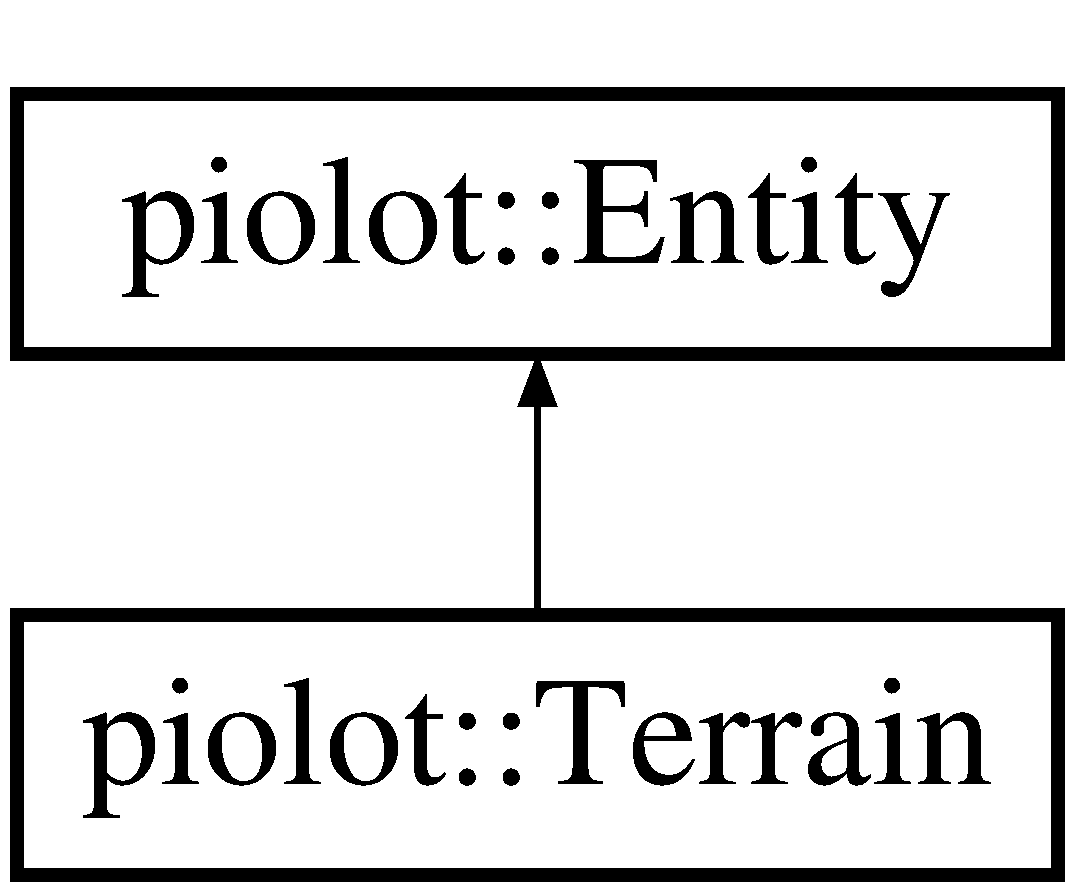
\includegraphics[height=2.000000cm]{classpiolot_1_1_entity}
\end{center}
\end{figure}
\subsection*{Public Member Functions}
\begin{DoxyCompactItemize}
\item 
\mbox{\Hypertarget{classpiolot_1_1_entity_afcf183909460f962951d9775126e35dc}\label{classpiolot_1_1_entity_afcf183909460f962951d9775126e35dc}} 
std\+::string {\bfseries Get\+Entity\+Name} () const
\item 
\mbox{\Hypertarget{classpiolot_1_1_entity_a4b458394b15a68f6ecf19e79b60f8730}\label{classpiolot_1_1_entity_a4b458394b15a68f6ecf19e79b60f8730}} 
void {\bfseries Set\+Entity\+Name} (const std\+::string \&entity\+\_\+name)
\item 
\mbox{\Hypertarget{classpiolot_1_1_entity_a1c52edf232af06086a4058c46d2cb783}\label{classpiolot_1_1_entity_a1c52edf232af06086a4058c46d2cb783}} 
void {\bfseries Set\+Shader\+Name} (const std\+::string \&shader\+\_\+name)
\item 
\mbox{\Hypertarget{classpiolot_1_1_entity_ae2f2a9ae6613e02d69129e5346884f4e}\label{classpiolot_1_1_entity_ae2f2a9ae6613e02d69129e5346884f4e}} 
bool {\bfseries Is\+Selected\+In\+Scene} () const
\item 
\mbox{\Hypertarget{classpiolot_1_1_entity_ab989dc8df66c461663c431993b5b2334}\label{classpiolot_1_1_entity_ab989dc8df66c461663c431993b5b2334}} 
void {\bfseries Set\+Selected\+In\+Scene} (bool \+\_\+selected\+In\+Scene)
\item 
\mbox{\Hypertarget{classpiolot_1_1_entity_a71f340517f503b0187e96e3f0097fdbc}\label{classpiolot_1_1_entity_a71f340517f503b0187e96e3f0097fdbc}} 
const \mbox{\hyperlink{classpiolot_1_1_bounding_box}{Bounding\+Box}} \& {\bfseries Get\+Bounding\+Box} () const
\item 
\mbox{\Hypertarget{classpiolot_1_1_entity_a95f3ad12bcec709938fb35633d51a3f5}\label{classpiolot_1_1_entity_a95f3ad12bcec709938fb35633d51a3f5}} 
const std\+::string \& {\bfseries Get\+Shader\+Name} () const
\item 
\mbox{\Hypertarget{classpiolot_1_1_entity_a575051c2dffebde6948c421bb9153c3c}\label{classpiolot_1_1_entity_a575051c2dffebde6948c421bb9153c3c}} 
void {\bfseries Set\+Object\+Name} (const std\+::string \&\+\_\+object\+Name)
\item 
\mbox{\Hypertarget{classpiolot_1_1_entity_a2eeb2cd5d0daf98c49b0e2d2d6227e6d}\label{classpiolot_1_1_entity_a2eeb2cd5d0daf98c49b0e2d2d6227e6d}} 
const std\+::string \& {\bfseries Get\+Object\+Name} () const
\item 
\mbox{\Hypertarget{classpiolot_1_1_entity_a9c38cdd359bfab2de36e2478d368a27e}\label{classpiolot_1_1_entity_a9c38cdd359bfab2de36e2478d368a27e}} 
const glm\+::vec3 \& {\bfseries Get\+Position} () const
\item 
\mbox{\Hypertarget{classpiolot_1_1_entity_a4cd721f2ff085908999d9c100bbaf214}\label{classpiolot_1_1_entity_a4cd721f2ff085908999d9c100bbaf214}} 
const glm\+::vec3 \& {\bfseries Get\+Rotation} () const
\item 
\mbox{\Hypertarget{classpiolot_1_1_entity_ac5530a0639da344c0e8f86c2176fa4a6}\label{classpiolot_1_1_entity_ac5530a0639da344c0e8f86c2176fa4a6}} 
const glm\+::vec3 \& {\bfseries Get\+Scale} () const
\item 
\mbox{\Hypertarget{classpiolot_1_1_entity_a6b0a54f38fa54989ad1c237d40fabcb0}\label{classpiolot_1_1_entity_a6b0a54f38fa54989ad1c237d40fabcb0}} 
const glm\+::mat4 \& {\bfseries Get\+Model\+Matrix} () const
\item 
\mbox{\Hypertarget{classpiolot_1_1_entity_a025d60f0f6de447381d9ab2211986075}\label{classpiolot_1_1_entity_a025d60f0f6de447381d9ab2211986075}} 
bool {\bfseries Is\+Matrix\+Dirty} () const
\item 
\mbox{\Hypertarget{classpiolot_1_1_entity_af80fc92eb9232113046c602d5daa1a76}\label{classpiolot_1_1_entity_af80fc92eb9232113046c602d5daa1a76}} 
void {\bfseries Set\+Position} (const glm\+::vec3 \&\+\_\+position)
\item 
\mbox{\Hypertarget{classpiolot_1_1_entity_ae2d789ed80e63f1bcad90d003ea15e94}\label{classpiolot_1_1_entity_ae2d789ed80e63f1bcad90d003ea15e94}} 
void {\bfseries Set\+Rotation} (const glm\+::vec3 \&\+\_\+rotation)
\item 
\mbox{\Hypertarget{classpiolot_1_1_entity_a16d7b329d92ebdc78178e460c7cee6dc}\label{classpiolot_1_1_entity_a16d7b329d92ebdc78178e460c7cee6dc}} 
void {\bfseries Set\+Scale} (const glm\+::vec3 \&\+\_\+scale)
\item 
\mbox{\Hypertarget{classpiolot_1_1_entity_ae7fc7ed3219c928da4bce17e1e504733}\label{classpiolot_1_1_entity_ae7fc7ed3219c928da4bce17e1e504733}} 
{\bfseries Entity} (const std\+::string \&\+\_\+object\+Path, const std\+::string \&\+\_\+shader\+Name)
\item 
\mbox{\Hypertarget{classpiolot_1_1_entity_a35aed98e4aedd0aa64ee512f83d912ec}\label{classpiolot_1_1_entity_a35aed98e4aedd0aa64ee512f83d912ec}} 
void {\bfseries Update} (float \+\_\+delta\+Time)
\item 
\mbox{\Hypertarget{classpiolot_1_1_entity_a9b7f0caf16313208ca115504a2453a12}\label{classpiolot_1_1_entity_a9b7f0caf16313208ca115504a2453a12}} 
void {\bfseries Render} ()
\item 
\mbox{\Hypertarget{classpiolot_1_1_entity_affee050e5904bd4dff3239804bea6e7e}\label{classpiolot_1_1_entity_affee050e5904bd4dff3239804bea6e7e}} 
bool {\bfseries Check\+If\+Mouse\+Overed} (const glm\+::vec3 \+\_\+camera\+Position, const glm\+::vec3 \+\_\+mouse\+Ray\+Direction, float \&\+\_\+distance) const
\item 
\mbox{\Hypertarget{classpiolot_1_1_entity_acc08eed4d3e1185dfc3fb396720443e5}\label{classpiolot_1_1_entity_acc08eed4d3e1185dfc3fb396720443e5}} 
void {\bfseries Display\+Details\+Imgui} ()
\end{DoxyCompactItemize}
\subsection*{Protected Member Functions}
\begin{DoxyCompactItemize}
\item 
\mbox{\Hypertarget{classpiolot_1_1_entity_a100b4699f74f506217c4d545f5a81f58}\label{classpiolot_1_1_entity_a100b4699f74f506217c4d545f5a81f58}} 
void {\bfseries Update\+Matrices} ()
\end{DoxyCompactItemize}
\subsection*{Protected Attributes}
\begin{DoxyCompactItemize}
\item 
\mbox{\Hypertarget{classpiolot_1_1_entity_aa2eeb64fbf3f1445b2895ac680ba7e36}\label{classpiolot_1_1_entity_aa2eeb64fbf3f1445b2895ac680ba7e36}} 
std\+::string {\bfseries shader\+Name}
\item 
\mbox{\Hypertarget{classpiolot_1_1_entity_a133cd55e173decca797dde8d6c4714d3}\label{classpiolot_1_1_entity_a133cd55e173decca797dde8d6c4714d3}} 
\mbox{\hyperlink{classpiolot_1_1_bounding_box}{Bounding\+Box}} {\bfseries bounding\+Box}
\item 
\mbox{\Hypertarget{classpiolot_1_1_entity_a50e4d7090890c7bedc3dffa1fe4d3dc9}\label{classpiolot_1_1_entity_a50e4d7090890c7bedc3dffa1fe4d3dc9}} 
bool {\bfseries selected\+In\+Scene} = false
\item 
\mbox{\Hypertarget{classpiolot_1_1_entity_acdc85c4db87446266e0e04392d54cd11}\label{classpiolot_1_1_entity_acdc85c4db87446266e0e04392d54cd11}} 
std\+::string {\bfseries entity\+Name}
\item 
\mbox{\Hypertarget{classpiolot_1_1_entity_a453c36793cfbab8662e28a8c10986432}\label{classpiolot_1_1_entity_a453c36793cfbab8662e28a8c10986432}} 
std\+::string {\bfseries object\+Name}
\item 
\mbox{\Hypertarget{classpiolot_1_1_entity_a1996e97527821230db17bc0c93a9ba26}\label{classpiolot_1_1_entity_a1996e97527821230db17bc0c93a9ba26}} 
glm\+::vec3 {\bfseries position} \{\}
\item 
\mbox{\Hypertarget{classpiolot_1_1_entity_ad490e079062ae866cbd14afbc768c37f}\label{classpiolot_1_1_entity_ad490e079062ae866cbd14afbc768c37f}} 
glm\+::vec3 {\bfseries rotation} \{0.\+0f, 0.\+0f, 0.\+0f\}
\item 
\mbox{\Hypertarget{classpiolot_1_1_entity_a80bbefe25b4316190caf5d8cc77bd125}\label{classpiolot_1_1_entity_a80bbefe25b4316190caf5d8cc77bd125}} 
glm\+::vec3 {\bfseries scale} \{1.\+0f, 1.\+0f, 1.\+0f\}
\item 
\mbox{\Hypertarget{classpiolot_1_1_entity_abca37f3906e85c0f184f1c2ffe627a7e}\label{classpiolot_1_1_entity_abca37f3906e85c0f184f1c2ffe627a7e}} 
glm\+::mat4 {\bfseries model\+Matrix} \{\}
\item 
\mbox{\Hypertarget{classpiolot_1_1_entity_ae8f4e05ad6742e55a3ed3792d21c3282}\label{classpiolot_1_1_entity_ae8f4e05ad6742e55a3ed3792d21c3282}} 
bool {\bfseries matrix\+Dirty} = true
\end{DoxyCompactItemize}


The documentation for this class was generated from the following files\+:\begin{DoxyCompactItemize}
\item 
C\+:/dev/\+Piolot/\+Engine/Entity.\+h\item 
C\+:/dev/\+Piolot/\+Engine/Entity.\+cpp\end{DoxyCompactItemize}

\hypertarget{classpiolot_1_1_g_l_shader}{}\section{piolot\+:\+:G\+L\+Shader Class Reference}
\label{classpiolot_1_1_g_l_shader}\index{piolot\+::\+G\+L\+Shader@{piolot\+::\+G\+L\+Shader}}


The Class that is used to load shaders in Open\+GL.  




{\ttfamily \#include $<$G\+L\+Shader.\+h$>$}

\subsection*{Public Member Functions}
\begin{DoxyCompactItemize}
\item 
\mbox{\hyperlink{classpiolot_1_1_g_l_shader_a9280ae5003e53461f898dd18b7685eab}{G\+L\+Shader}} (const char $\ast$\+\_\+vertex\+Path, const char $\ast$\+\_\+fragment\+Path)
\begin{DoxyCompactList}\small\item\em Loads the shader at the specified path. \end{DoxyCompactList}\item 
\mbox{\Hypertarget{classpiolot_1_1_g_l_shader_a1ed833e8b2ade593d5c820981121bfbb}\label{classpiolot_1_1_g_l_shader_a1ed833e8b2ade593d5c820981121bfbb}} 
{\bfseries G\+L\+Shader} (const char $\ast$\+\_\+file\+Path)
\item 
\mbox{\Hypertarget{classpiolot_1_1_g_l_shader_a7bf14037e4f1f1e5b6af344da08d6430}\label{classpiolot_1_1_g_l_shader_a7bf14037e4f1f1e5b6af344da08d6430}} 
\mbox{\hyperlink{classpiolot_1_1_g_l_shader_a7bf14037e4f1f1e5b6af344da08d6430}{$\sim$\+G\+L\+Shader}} ()=default
\begin{DoxyCompactList}\small\item\em Default Destructor. \end{DoxyCompactList}\item 
\mbox{\Hypertarget{classpiolot_1_1_g_l_shader_a624427668ba51101fe898e12731069bf}\label{classpiolot_1_1_g_l_shader_a624427668ba51101fe898e12731069bf}} 
void \mbox{\hyperlink{classpiolot_1_1_g_l_shader_a624427668ba51101fe898e12731069bf}{use}} ()
\begin{DoxyCompactList}\small\item\em Use the Program. \end{DoxyCompactList}\item 
void \mbox{\hyperlink{classpiolot_1_1_g_l_shader_a8f3349b73adbb3f7d85b847ffc39d0f3}{set\+Bool}} (const std\+::string \&\+\_\+name, bool \+\_\+value)
\begin{DoxyCompactList}\small\item\em Set a Uniform Value. \end{DoxyCompactList}\item 
void \mbox{\hyperlink{classpiolot_1_1_g_l_shader_a5b8fd3a108bf576243a1e852872edf5c}{set\+Int}} (const std\+::string \&\+\_\+name, int \+\_\+value)
\begin{DoxyCompactList}\small\item\em Set a Uniform Value. \end{DoxyCompactList}\item 
void \mbox{\hyperlink{classpiolot_1_1_g_l_shader_af6323e1d0956064de4c43ef4fa41b0f1}{set\+Float}} (const std\+::string \&\+\_\+name, float \+\_\+value)
\begin{DoxyCompactList}\small\item\em Set a Uniform Value. \end{DoxyCompactList}\item 
void \mbox{\hyperlink{classpiolot_1_1_g_l_shader_a47d614244dc667768a36b9cea1675eca}{set\+Vec3}} (const std\+::string \&\+\_\+name, const glm\+::vec3 \&\+\_\+value)
\begin{DoxyCompactList}\small\item\em Set a Uniform Value. \end{DoxyCompactList}\item 
void \mbox{\hyperlink{classpiolot_1_1_g_l_shader_a293369149f4ad507543cb0fcd783afd1}{set\+Vec3}} (const std\+::string \&\+\_\+name, float \+\_\+x, float \+\_\+y, float \+\_\+z)
\begin{DoxyCompactList}\small\item\em Set a Uniform Value. \end{DoxyCompactList}\item 
void \mbox{\hyperlink{classpiolot_1_1_g_l_shader_a56d846ae1d7c6adc579c5de37db02546}{set\+Mat4}} (const std\+::string \&\+\_\+name, const glm\+::mat4 \&\+\_\+mat)
\begin{DoxyCompactList}\small\item\em Set a Uniform Value. \end{DoxyCompactList}\item 
bool \mbox{\hyperlink{classpiolot_1_1_g_l_shader_ab2badc2b316c708bf6ea7a4ff39db254}{Check\+Compile\+Errors}} (unsigned int \+\_\+shader\+Id, std\+::string \+\_\+type)
\begin{DoxyCompactList}\small\item\em Check for any Compilation Errors and report. \end{DoxyCompactList}\item 
\mbox{\Hypertarget{classpiolot_1_1_g_l_shader_ac5bf2e67deb4f816e82a50bbe1f168dd}\label{classpiolot_1_1_g_l_shader_ac5bf2e67deb4f816e82a50bbe1f168dd}} 
int {\bfseries Get\+Uniform\+Location} (const std\+::string \&\+\_\+name)
\end{DoxyCompactItemize}
\subsection*{Public Attributes}
\begin{DoxyCompactItemize}
\item 
\mbox{\Hypertarget{classpiolot_1_1_g_l_shader_a7f05981084b76212d3ee92c71e002fb2}\label{classpiolot_1_1_g_l_shader_a7f05981084b76212d3ee92c71e002fb2}} 
unsigned int \mbox{\hyperlink{classpiolot_1_1_g_l_shader_a7f05981084b76212d3ee92c71e002fb2}{shader\+Id}}
\begin{DoxyCompactList}\small\item\em The Shader ID that you get once you load the Shader. \end{DoxyCompactList}\item 
\mbox{\Hypertarget{classpiolot_1_1_g_l_shader_af6cacc0e6d324c39ec3b862dc0ff29a8}\label{classpiolot_1_1_g_l_shader_af6cacc0e6d324c39ec3b862dc0ff29a8}} 
std\+::string {\bfseries shader\+Name}
\item 
\mbox{\Hypertarget{classpiolot_1_1_g_l_shader_aa99f7e5b6b76e8796824278578e4172d}\label{classpiolot_1_1_g_l_shader_aa99f7e5b6b76e8796824278578e4172d}} 
bool {\bfseries compile\+Status} = true
\item 
\mbox{\Hypertarget{classpiolot_1_1_g_l_shader_adde3ba01aacd0c60bd495ca3b220a1dd}\label{classpiolot_1_1_g_l_shader_adde3ba01aacd0c60bd495ca3b220a1dd}} 
std\+::unordered\+\_\+map$<$ std\+::string, int $>$ {\bfseries uniform\+Locations}
\end{DoxyCompactItemize}


\subsection{Detailed Description}
The Class that is used to load shaders in Open\+GL. 

\subsection{Constructor \& Destructor Documentation}
\mbox{\Hypertarget{classpiolot_1_1_g_l_shader_a9280ae5003e53461f898dd18b7685eab}\label{classpiolot_1_1_g_l_shader_a9280ae5003e53461f898dd18b7685eab}} 
\index{piolot\+::\+G\+L\+Shader@{piolot\+::\+G\+L\+Shader}!G\+L\+Shader@{G\+L\+Shader}}
\index{G\+L\+Shader@{G\+L\+Shader}!piolot\+::\+G\+L\+Shader@{piolot\+::\+G\+L\+Shader}}
\subsubsection{\texorpdfstring{G\+L\+Shader()}{GLShader()}}
{\footnotesize\ttfamily piolot\+::\+G\+L\+Shader\+::\+G\+L\+Shader (\begin{DoxyParamCaption}\item[{const char $\ast$}]{\+\_\+vertex\+Path,  }\item[{const char $\ast$}]{\+\_\+fragment\+Path }\end{DoxyParamCaption})}



Loads the shader at the specified path. 


\begin{DoxyParams}{Parameters}
{\em \+\_\+vertex\+Path} & The Vertex\+Shader Path \\
\hline
{\em \+\_\+fragment\+Path} & The Fragment Shader Path.\\
\hline
\end{DoxyParams}

\begin{DoxyItemize}
\item Reads the files specified by Shaderpaths.
\item Creates the Shaders and Compiles them.
\item Creates the Program and links the shaders.
\item Deletes the Shaders once the Program is successfully created.
\item Outputs any errors to the debug file. 
\end{DoxyItemize}

\subsection{Member Function Documentation}
\mbox{\Hypertarget{classpiolot_1_1_g_l_shader_ab2badc2b316c708bf6ea7a4ff39db254}\label{classpiolot_1_1_g_l_shader_ab2badc2b316c708bf6ea7a4ff39db254}} 
\index{piolot\+::\+G\+L\+Shader@{piolot\+::\+G\+L\+Shader}!Check\+Compile\+Errors@{Check\+Compile\+Errors}}
\index{Check\+Compile\+Errors@{Check\+Compile\+Errors}!piolot\+::\+G\+L\+Shader@{piolot\+::\+G\+L\+Shader}}
\subsubsection{\texorpdfstring{Check\+Compile\+Errors()}{CheckCompileErrors()}}
{\footnotesize\ttfamily bool piolot\+::\+G\+L\+Shader\+::\+Check\+Compile\+Errors (\begin{DoxyParamCaption}\item[{unsigned int}]{\+\_\+shader\+Id,  }\item[{std\+::string}]{\+\_\+type }\end{DoxyParamCaption})}



Check for any Compilation Errors and report. 


\begin{DoxyParams}{Parameters}
{\em \+\_\+shader\+Id} & The Shader/\+Program Id that we are checking the errors for. \\
\hline
{\em \+\_\+type} & The Type, Can be either P\+R\+O\+G\+R\+AM or S\+H\+A\+D\+ER. \\
\hline
\end{DoxyParams}
\mbox{\Hypertarget{classpiolot_1_1_g_l_shader_a8f3349b73adbb3f7d85b847ffc39d0f3}\label{classpiolot_1_1_g_l_shader_a8f3349b73adbb3f7d85b847ffc39d0f3}} 
\index{piolot\+::\+G\+L\+Shader@{piolot\+::\+G\+L\+Shader}!set\+Bool@{set\+Bool}}
\index{set\+Bool@{set\+Bool}!piolot\+::\+G\+L\+Shader@{piolot\+::\+G\+L\+Shader}}
\subsubsection{\texorpdfstring{set\+Bool()}{setBool()}}
{\footnotesize\ttfamily void piolot\+::\+G\+L\+Shader\+::set\+Bool (\begin{DoxyParamCaption}\item[{const std\+::string \&}]{\+\_\+name,  }\item[{bool}]{\+\_\+value }\end{DoxyParamCaption})\hspace{0.3cm}{\ttfamily [inline]}}



Set a Uniform Value. 


\begin{DoxyParams}{Parameters}
{\em \+\_\+name} & The Uniform Name \\
\hline
{\em \+\_\+value} & The Uniform Value. \\
\hline
\end{DoxyParams}
\mbox{\Hypertarget{classpiolot_1_1_g_l_shader_af6323e1d0956064de4c43ef4fa41b0f1}\label{classpiolot_1_1_g_l_shader_af6323e1d0956064de4c43ef4fa41b0f1}} 
\index{piolot\+::\+G\+L\+Shader@{piolot\+::\+G\+L\+Shader}!set\+Float@{set\+Float}}
\index{set\+Float@{set\+Float}!piolot\+::\+G\+L\+Shader@{piolot\+::\+G\+L\+Shader}}
\subsubsection{\texorpdfstring{set\+Float()}{setFloat()}}
{\footnotesize\ttfamily void piolot\+::\+G\+L\+Shader\+::set\+Float (\begin{DoxyParamCaption}\item[{const std\+::string \&}]{\+\_\+name,  }\item[{float}]{\+\_\+value }\end{DoxyParamCaption})\hspace{0.3cm}{\ttfamily [inline]}}



Set a Uniform Value. 


\begin{DoxyParams}{Parameters}
{\em \+\_\+name} & The Uniform Name \\
\hline
{\em \+\_\+value} & The Uniform Value. \\
\hline
\end{DoxyParams}
\mbox{\Hypertarget{classpiolot_1_1_g_l_shader_a5b8fd3a108bf576243a1e852872edf5c}\label{classpiolot_1_1_g_l_shader_a5b8fd3a108bf576243a1e852872edf5c}} 
\index{piolot\+::\+G\+L\+Shader@{piolot\+::\+G\+L\+Shader}!set\+Int@{set\+Int}}
\index{set\+Int@{set\+Int}!piolot\+::\+G\+L\+Shader@{piolot\+::\+G\+L\+Shader}}
\subsubsection{\texorpdfstring{set\+Int()}{setInt()}}
{\footnotesize\ttfamily void piolot\+::\+G\+L\+Shader\+::set\+Int (\begin{DoxyParamCaption}\item[{const std\+::string \&}]{\+\_\+name,  }\item[{int}]{\+\_\+value }\end{DoxyParamCaption})\hspace{0.3cm}{\ttfamily [inline]}}



Set a Uniform Value. 


\begin{DoxyParams}{Parameters}
{\em \+\_\+name} & The Uniform Name \\
\hline
{\em \+\_\+value} & The Uniform Value. \\
\hline
\end{DoxyParams}
\mbox{\Hypertarget{classpiolot_1_1_g_l_shader_a56d846ae1d7c6adc579c5de37db02546}\label{classpiolot_1_1_g_l_shader_a56d846ae1d7c6adc579c5de37db02546}} 
\index{piolot\+::\+G\+L\+Shader@{piolot\+::\+G\+L\+Shader}!set\+Mat4@{set\+Mat4}}
\index{set\+Mat4@{set\+Mat4}!piolot\+::\+G\+L\+Shader@{piolot\+::\+G\+L\+Shader}}
\subsubsection{\texorpdfstring{set\+Mat4()}{setMat4()}}
{\footnotesize\ttfamily void piolot\+::\+G\+L\+Shader\+::set\+Mat4 (\begin{DoxyParamCaption}\item[{const std\+::string \&}]{\+\_\+name,  }\item[{const glm\+::mat4 \&}]{\+\_\+mat }\end{DoxyParamCaption})\hspace{0.3cm}{\ttfamily [inline]}}



Set a Uniform Value. 


\begin{DoxyParams}{Parameters}
{\em \+\_\+name} & The Uniform Name \\
\hline
{\em \+\_\+mat} & The Uniform Value. \\
\hline
\end{DoxyParams}
\mbox{\Hypertarget{classpiolot_1_1_g_l_shader_a47d614244dc667768a36b9cea1675eca}\label{classpiolot_1_1_g_l_shader_a47d614244dc667768a36b9cea1675eca}} 
\index{piolot\+::\+G\+L\+Shader@{piolot\+::\+G\+L\+Shader}!set\+Vec3@{set\+Vec3}}
\index{set\+Vec3@{set\+Vec3}!piolot\+::\+G\+L\+Shader@{piolot\+::\+G\+L\+Shader}}
\subsubsection{\texorpdfstring{set\+Vec3()}{setVec3()}\hspace{0.1cm}{\footnotesize\ttfamily [1/2]}}
{\footnotesize\ttfamily void piolot\+::\+G\+L\+Shader\+::set\+Vec3 (\begin{DoxyParamCaption}\item[{const std\+::string \&}]{\+\_\+name,  }\item[{const glm\+::vec3 \&}]{\+\_\+value }\end{DoxyParamCaption})\hspace{0.3cm}{\ttfamily [inline]}}



Set a Uniform Value. 


\begin{DoxyParams}{Parameters}
{\em \+\_\+name} & The Uniform Name \\
\hline
{\em \+\_\+value} & The Uniform Value. \\
\hline
\end{DoxyParams}
\mbox{\Hypertarget{classpiolot_1_1_g_l_shader_a293369149f4ad507543cb0fcd783afd1}\label{classpiolot_1_1_g_l_shader_a293369149f4ad507543cb0fcd783afd1}} 
\index{piolot\+::\+G\+L\+Shader@{piolot\+::\+G\+L\+Shader}!set\+Vec3@{set\+Vec3}}
\index{set\+Vec3@{set\+Vec3}!piolot\+::\+G\+L\+Shader@{piolot\+::\+G\+L\+Shader}}
\subsubsection{\texorpdfstring{set\+Vec3()}{setVec3()}\hspace{0.1cm}{\footnotesize\ttfamily [2/2]}}
{\footnotesize\ttfamily void piolot\+::\+G\+L\+Shader\+::set\+Vec3 (\begin{DoxyParamCaption}\item[{const std\+::string \&}]{\+\_\+name,  }\item[{float}]{\+\_\+x,  }\item[{float}]{\+\_\+y,  }\item[{float}]{\+\_\+z }\end{DoxyParamCaption})\hspace{0.3cm}{\ttfamily [inline]}}



Set a Uniform Value. 


\begin{DoxyParams}{Parameters}
{\em \+\_\+name} & The Uniform Name \\
\hline
{\em \+\_\+x} & Value.\+x \\
\hline
{\em \+\_\+y} & Value.\+y \\
\hline
{\em \+\_\+z} & Value.\+z \\
\hline
\end{DoxyParams}


The documentation for this class was generated from the following files\+:\begin{DoxyCompactItemize}
\item 
C\+:/dev/\+Piolot/\+Engine/G\+L\+Shader.\+h\item 
C\+:/dev/\+Piolot/\+Engine/G\+L\+Shader.\+cpp\end{DoxyCompactItemize}

\hypertarget{classpiolot_1_1_grid}{}\section{piolot\+:\+:Grid Class Reference}
\label{classpiolot_1_1_grid}\index{piolot\+::\+Grid@{piolot\+::\+Grid}}


{\ttfamily \#include $<$Grid.\+h$>$}

\subsection*{Public Member Functions}
\begin{DoxyCompactItemize}
\item 
\mbox{\hyperlink{classpiolot_1_1_grid_ab43feb8d7b505cf880c6d328aabe1adf}{Grid}} ()=default
\item 
void \mbox{\hyperlink{classpiolot_1_1_grid_acde85bc00911a143d9407a814e1d6d88}{Init}} ()
\item 
void \mbox{\hyperlink{classpiolot_1_1_grid_a3af0ba487e81a5d616788cd5f4ecbd11}{Update}} (const glm\+::mat4 \+\_\+view\+Matrix, const glm\+::mat4 \+\_\+projection\+Matrix)
\item 
void \mbox{\hyperlink{classpiolot_1_1_grid_a36c9dfed35987b298ca3bf4ff3cb06a8}{Render}} () const
\end{DoxyCompactItemize}
\subsection*{Public Attributes}
\begin{DoxyCompactItemize}
\item 
std\+::vector$<$ \mbox{\hyperlink{classpiolot_1_1_ray}{Ray}} $>$ \mbox{\hyperlink{classpiolot_1_1_grid_a09e5317cee1cd166c91363d608bde97d}{x\+\_\+rays}}
\item 
std\+::vector$<$ \mbox{\hyperlink{classpiolot_1_1_ray}{Ray}} $>$ \mbox{\hyperlink{classpiolot_1_1_grid_a8eaf3716e1f5623d15fa26cf1e8b2778}{y\+\_\+rays}}
\item 
std\+::vector$<$ \mbox{\hyperlink{classpiolot_1_1_ray}{Ray}} $>$ \mbox{\hyperlink{classpiolot_1_1_grid_a9407fb2aa26aae50604cd8d8197d3fb6}{z\+\_\+rays}}
\item 
glm\+::mat4 \mbox{\hyperlink{classpiolot_1_1_grid_acc61d6d0bc8d0b7cf77da8193f40433e}{view\+Matrix}}
\item 
glm\+::mat4 \mbox{\hyperlink{classpiolot_1_1_grid_ada577e74647a548fb07af5bd8597d6d8}{projection\+Matrix}}
\item 
std\+::shared\+\_\+ptr$<$ \mbox{\hyperlink{classpiolot_1_1_g_l_shader}{G\+L\+Shader}} $>$ \mbox{\hyperlink{classpiolot_1_1_grid_a3eaeeee54a7aef5807b8927b1ca2615e}{shader}}
\end{DoxyCompactItemize}


\subsection{Constructor \& Destructor Documentation}
\mbox{\Hypertarget{classpiolot_1_1_grid_ab43feb8d7b505cf880c6d328aabe1adf}\label{classpiolot_1_1_grid_ab43feb8d7b505cf880c6d328aabe1adf}} 
\index{piolot\+::\+Grid@{piolot\+::\+Grid}!Grid@{Grid}}
\index{Grid@{Grid}!piolot\+::\+Grid@{piolot\+::\+Grid}}
\subsubsection{\texorpdfstring{Grid()}{Grid()}}
{\footnotesize\ttfamily piolot\+::\+Grid\+::\+Grid (\begin{DoxyParamCaption}{ }\end{DoxyParamCaption})\hspace{0.3cm}{\ttfamily [default]}}



\subsection{Member Function Documentation}
\mbox{\Hypertarget{classpiolot_1_1_grid_acde85bc00911a143d9407a814e1d6d88}\label{classpiolot_1_1_grid_acde85bc00911a143d9407a814e1d6d88}} 
\index{piolot\+::\+Grid@{piolot\+::\+Grid}!Init@{Init}}
\index{Init@{Init}!piolot\+::\+Grid@{piolot\+::\+Grid}}
\subsubsection{\texorpdfstring{Init()}{Init()}}
{\footnotesize\ttfamily void piolot\+::\+Grid\+::\+Init (\begin{DoxyParamCaption}{ }\end{DoxyParamCaption})}

\mbox{\Hypertarget{classpiolot_1_1_grid_a36c9dfed35987b298ca3bf4ff3cb06a8}\label{classpiolot_1_1_grid_a36c9dfed35987b298ca3bf4ff3cb06a8}} 
\index{piolot\+::\+Grid@{piolot\+::\+Grid}!Render@{Render}}
\index{Render@{Render}!piolot\+::\+Grid@{piolot\+::\+Grid}}
\subsubsection{\texorpdfstring{Render()}{Render()}}
{\footnotesize\ttfamily void piolot\+::\+Grid\+::\+Render (\begin{DoxyParamCaption}{ }\end{DoxyParamCaption}) const}

\mbox{\Hypertarget{classpiolot_1_1_grid_a3af0ba487e81a5d616788cd5f4ecbd11}\label{classpiolot_1_1_grid_a3af0ba487e81a5d616788cd5f4ecbd11}} 
\index{piolot\+::\+Grid@{piolot\+::\+Grid}!Update@{Update}}
\index{Update@{Update}!piolot\+::\+Grid@{piolot\+::\+Grid}}
\subsubsection{\texorpdfstring{Update()}{Update()}}
{\footnotesize\ttfamily void piolot\+::\+Grid\+::\+Update (\begin{DoxyParamCaption}\item[{const glm\+::mat4}]{\+\_\+view\+Matrix,  }\item[{const glm\+::mat4}]{\+\_\+projection\+Matrix }\end{DoxyParamCaption})}



\subsection{Member Data Documentation}
\mbox{\Hypertarget{classpiolot_1_1_grid_ada577e74647a548fb07af5bd8597d6d8}\label{classpiolot_1_1_grid_ada577e74647a548fb07af5bd8597d6d8}} 
\index{piolot\+::\+Grid@{piolot\+::\+Grid}!projection\+Matrix@{projection\+Matrix}}
\index{projection\+Matrix@{projection\+Matrix}!piolot\+::\+Grid@{piolot\+::\+Grid}}
\subsubsection{\texorpdfstring{projection\+Matrix}{projectionMatrix}}
{\footnotesize\ttfamily glm\+::mat4 piolot\+::\+Grid\+::projection\+Matrix}

\mbox{\Hypertarget{classpiolot_1_1_grid_a3eaeeee54a7aef5807b8927b1ca2615e}\label{classpiolot_1_1_grid_a3eaeeee54a7aef5807b8927b1ca2615e}} 
\index{piolot\+::\+Grid@{piolot\+::\+Grid}!shader@{shader}}
\index{shader@{shader}!piolot\+::\+Grid@{piolot\+::\+Grid}}
\subsubsection{\texorpdfstring{shader}{shader}}
{\footnotesize\ttfamily std\+::shared\+\_\+ptr$<$\mbox{\hyperlink{classpiolot_1_1_g_l_shader}{G\+L\+Shader}}$>$ piolot\+::\+Grid\+::shader}

\mbox{\Hypertarget{classpiolot_1_1_grid_acc61d6d0bc8d0b7cf77da8193f40433e}\label{classpiolot_1_1_grid_acc61d6d0bc8d0b7cf77da8193f40433e}} 
\index{piolot\+::\+Grid@{piolot\+::\+Grid}!view\+Matrix@{view\+Matrix}}
\index{view\+Matrix@{view\+Matrix}!piolot\+::\+Grid@{piolot\+::\+Grid}}
\subsubsection{\texorpdfstring{view\+Matrix}{viewMatrix}}
{\footnotesize\ttfamily glm\+::mat4 piolot\+::\+Grid\+::view\+Matrix}

\mbox{\Hypertarget{classpiolot_1_1_grid_a09e5317cee1cd166c91363d608bde97d}\label{classpiolot_1_1_grid_a09e5317cee1cd166c91363d608bde97d}} 
\index{piolot\+::\+Grid@{piolot\+::\+Grid}!x\+\_\+rays@{x\+\_\+rays}}
\index{x\+\_\+rays@{x\+\_\+rays}!piolot\+::\+Grid@{piolot\+::\+Grid}}
\subsubsection{\texorpdfstring{x\+\_\+rays}{x\_rays}}
{\footnotesize\ttfamily std\+::vector$<$\mbox{\hyperlink{classpiolot_1_1_ray}{Ray}}$>$ piolot\+::\+Grid\+::x\+\_\+rays}

\mbox{\Hypertarget{classpiolot_1_1_grid_a8eaf3716e1f5623d15fa26cf1e8b2778}\label{classpiolot_1_1_grid_a8eaf3716e1f5623d15fa26cf1e8b2778}} 
\index{piolot\+::\+Grid@{piolot\+::\+Grid}!y\+\_\+rays@{y\+\_\+rays}}
\index{y\+\_\+rays@{y\+\_\+rays}!piolot\+::\+Grid@{piolot\+::\+Grid}}
\subsubsection{\texorpdfstring{y\+\_\+rays}{y\_rays}}
{\footnotesize\ttfamily std\+::vector$<$\mbox{\hyperlink{classpiolot_1_1_ray}{Ray}}$>$ piolot\+::\+Grid\+::y\+\_\+rays}

\mbox{\Hypertarget{classpiolot_1_1_grid_a9407fb2aa26aae50604cd8d8197d3fb6}\label{classpiolot_1_1_grid_a9407fb2aa26aae50604cd8d8197d3fb6}} 
\index{piolot\+::\+Grid@{piolot\+::\+Grid}!z\+\_\+rays@{z\+\_\+rays}}
\index{z\+\_\+rays@{z\+\_\+rays}!piolot\+::\+Grid@{piolot\+::\+Grid}}
\subsubsection{\texorpdfstring{z\+\_\+rays}{z\_rays}}
{\footnotesize\ttfamily std\+::vector$<$\mbox{\hyperlink{classpiolot_1_1_ray}{Ray}}$>$ piolot\+::\+Grid\+::z\+\_\+rays}



The documentation for this class was generated from the following files\+:\begin{DoxyCompactItemize}
\item 
\mbox{\hyperlink{_grid_8h}{Grid.\+h}}\item 
\mbox{\hyperlink{_grid_8cpp}{Grid.\+cpp}}\end{DoxyCompactItemize}

\hypertarget{structpiolot_1_1_im_gui_control_variables}{}\section{piolot\+:\+:Im\+Gui\+Control\+Variables Struct Reference}
\label{structpiolot_1_1_im_gui_control_variables}\index{piolot\+::\+Im\+Gui\+Control\+Variables@{piolot\+::\+Im\+Gui\+Control\+Variables}}
\subsection*{Public Attributes}
\begin{DoxyCompactItemize}
\item 
\mbox{\Hypertarget{structpiolot_1_1_im_gui_control_variables_ae4b05c60d0566aae16e8ab68980b473d}\label{structpiolot_1_1_im_gui_control_variables_ae4b05c60d0566aae16e8ab68980b473d}} 
bool \& {\bfseries show\+\_\+multiple\+\_\+viewports}
\end{DoxyCompactItemize}


The documentation for this struct was generated from the following file\+:\begin{DoxyCompactItemize}
\item 
C\+:/dev/\+Piolot/\+Engine/Test\+Scene.\+h\end{DoxyCompactItemize}

\hypertarget{structpiolot_1_1_im_gui_log}{}\section{piolot\+:\+:Im\+Gui\+Log Struct Reference}
\label{structpiolot_1_1_im_gui_log}\index{piolot\+::\+Im\+Gui\+Log@{piolot\+::\+Im\+Gui\+Log}}


{\ttfamily \#include $<$G\+U\+I\+Helpers.\+h$>$}

\subsection*{Public Member Functions}
\begin{DoxyCompactItemize}
\item 
void \mbox{\hyperlink{structpiolot_1_1_im_gui_log_ac7812f01c1da335a594a88e9b5d417f5}{Clear}} ()
\item 
void \mbox{\hyperlink{structpiolot_1_1_im_gui_log_a29f527cccbe3946d24c8098ccf871699}{Add\+Log}} (const char $\ast$fmt,...) I\+M\+\_\+\+F\+M\+T\+A\+R\+GS(2)
\item 
void \mbox{\hyperlink{structpiolot_1_1_im_gui_log_adaab8c65a0a76e8b434ae0edc4834a36}{Draw}} (const char $\ast$title, bool $\ast$p\+\_\+open=N\+U\+LL)
\end{DoxyCompactItemize}
\subsection*{Public Attributes}
\begin{DoxyCompactItemize}
\item 
Im\+Gui\+Text\+Buffer \mbox{\hyperlink{structpiolot_1_1_im_gui_log_a0e64a8554125f6a918016325996c8a28}{Buf}}
\item 
Im\+Gui\+Text\+Filter \mbox{\hyperlink{structpiolot_1_1_im_gui_log_a2649c271372b11fbf1f8fd5ebdec6055}{Filter}}
\item 
Im\+Vector$<$ int $>$ \mbox{\hyperlink{structpiolot_1_1_im_gui_log_a8c942c870cf5599fee50d7d7d30152b0}{Line\+Offsets}}
\item 
bool \mbox{\hyperlink{structpiolot_1_1_im_gui_log_ae6efe1280bb054ee0651ad47251f4457}{Scroll\+To\+Bottom}}
\end{DoxyCompactItemize}


\subsection{Member Function Documentation}
\mbox{\Hypertarget{structpiolot_1_1_im_gui_log_a29f527cccbe3946d24c8098ccf871699}\label{structpiolot_1_1_im_gui_log_a29f527cccbe3946d24c8098ccf871699}} 
\index{piolot\+::\+Im\+Gui\+Log@{piolot\+::\+Im\+Gui\+Log}!Add\+Log@{Add\+Log}}
\index{Add\+Log@{Add\+Log}!piolot\+::\+Im\+Gui\+Log@{piolot\+::\+Im\+Gui\+Log}}
\subsubsection{\texorpdfstring{Add\+Log()}{AddLog()}}
{\footnotesize\ttfamily void piolot\+::\+Im\+Gui\+Log\+::\+Add\+Log (\begin{DoxyParamCaption}\item[{const char $\ast$}]{fmt,  }\item[{}]{... }\end{DoxyParamCaption})\hspace{0.3cm}{\ttfamily [inline]}}

\mbox{\Hypertarget{structpiolot_1_1_im_gui_log_ac7812f01c1da335a594a88e9b5d417f5}\label{structpiolot_1_1_im_gui_log_ac7812f01c1da335a594a88e9b5d417f5}} 
\index{piolot\+::\+Im\+Gui\+Log@{piolot\+::\+Im\+Gui\+Log}!Clear@{Clear}}
\index{Clear@{Clear}!piolot\+::\+Im\+Gui\+Log@{piolot\+::\+Im\+Gui\+Log}}
\subsubsection{\texorpdfstring{Clear()}{Clear()}}
{\footnotesize\ttfamily void piolot\+::\+Im\+Gui\+Log\+::\+Clear (\begin{DoxyParamCaption}{ }\end{DoxyParamCaption})\hspace{0.3cm}{\ttfamily [inline]}}

\mbox{\Hypertarget{structpiolot_1_1_im_gui_log_adaab8c65a0a76e8b434ae0edc4834a36}\label{structpiolot_1_1_im_gui_log_adaab8c65a0a76e8b434ae0edc4834a36}} 
\index{piolot\+::\+Im\+Gui\+Log@{piolot\+::\+Im\+Gui\+Log}!Draw@{Draw}}
\index{Draw@{Draw}!piolot\+::\+Im\+Gui\+Log@{piolot\+::\+Im\+Gui\+Log}}
\subsubsection{\texorpdfstring{Draw()}{Draw()}}
{\footnotesize\ttfamily void piolot\+::\+Im\+Gui\+Log\+::\+Draw (\begin{DoxyParamCaption}\item[{const char $\ast$}]{title,  }\item[{bool $\ast$}]{p\+\_\+open = {\ttfamily NULL} }\end{DoxyParamCaption})\hspace{0.3cm}{\ttfamily [inline]}}



\subsection{Member Data Documentation}
\mbox{\Hypertarget{structpiolot_1_1_im_gui_log_a0e64a8554125f6a918016325996c8a28}\label{structpiolot_1_1_im_gui_log_a0e64a8554125f6a918016325996c8a28}} 
\index{piolot\+::\+Im\+Gui\+Log@{piolot\+::\+Im\+Gui\+Log}!Buf@{Buf}}
\index{Buf@{Buf}!piolot\+::\+Im\+Gui\+Log@{piolot\+::\+Im\+Gui\+Log}}
\subsubsection{\texorpdfstring{Buf}{Buf}}
{\footnotesize\ttfamily Im\+Gui\+Text\+Buffer piolot\+::\+Im\+Gui\+Log\+::\+Buf}

\mbox{\Hypertarget{structpiolot_1_1_im_gui_log_a2649c271372b11fbf1f8fd5ebdec6055}\label{structpiolot_1_1_im_gui_log_a2649c271372b11fbf1f8fd5ebdec6055}} 
\index{piolot\+::\+Im\+Gui\+Log@{piolot\+::\+Im\+Gui\+Log}!Filter@{Filter}}
\index{Filter@{Filter}!piolot\+::\+Im\+Gui\+Log@{piolot\+::\+Im\+Gui\+Log}}
\subsubsection{\texorpdfstring{Filter}{Filter}}
{\footnotesize\ttfamily Im\+Gui\+Text\+Filter piolot\+::\+Im\+Gui\+Log\+::\+Filter}

\mbox{\Hypertarget{structpiolot_1_1_im_gui_log_a8c942c870cf5599fee50d7d7d30152b0}\label{structpiolot_1_1_im_gui_log_a8c942c870cf5599fee50d7d7d30152b0}} 
\index{piolot\+::\+Im\+Gui\+Log@{piolot\+::\+Im\+Gui\+Log}!Line\+Offsets@{Line\+Offsets}}
\index{Line\+Offsets@{Line\+Offsets}!piolot\+::\+Im\+Gui\+Log@{piolot\+::\+Im\+Gui\+Log}}
\subsubsection{\texorpdfstring{Line\+Offsets}{LineOffsets}}
{\footnotesize\ttfamily Im\+Vector$<$int$>$ piolot\+::\+Im\+Gui\+Log\+::\+Line\+Offsets}

\mbox{\Hypertarget{structpiolot_1_1_im_gui_log_ae6efe1280bb054ee0651ad47251f4457}\label{structpiolot_1_1_im_gui_log_ae6efe1280bb054ee0651ad47251f4457}} 
\index{piolot\+::\+Im\+Gui\+Log@{piolot\+::\+Im\+Gui\+Log}!Scroll\+To\+Bottom@{Scroll\+To\+Bottom}}
\index{Scroll\+To\+Bottom@{Scroll\+To\+Bottom}!piolot\+::\+Im\+Gui\+Log@{piolot\+::\+Im\+Gui\+Log}}
\subsubsection{\texorpdfstring{Scroll\+To\+Bottom}{ScrollToBottom}}
{\footnotesize\ttfamily bool piolot\+::\+Im\+Gui\+Log\+::\+Scroll\+To\+Bottom}



The documentation for this struct was generated from the following file\+:\begin{DoxyCompactItemize}
\item 
\mbox{\hyperlink{_g_u_i_helpers_8h}{G\+U\+I\+Helpers.\+h}}\end{DoxyCompactItemize}

\hypertarget{classpiolot_1_1_logging_manager}{}\section{piolot\+:\+:Logging\+Manager Class Reference}
\label{classpiolot_1_1_logging_manager}\index{piolot\+::\+Logging\+Manager@{piolot\+::\+Logging\+Manager}}
\subsection*{Public Member Functions}
\begin{DoxyCompactItemize}
\item 
\mbox{\Hypertarget{classpiolot_1_1_logging_manager_aa0a0a7241a2d993282a18d7a8bded2ac}\label{classpiolot_1_1_logging_manager_aa0a0a7241a2d993282a18d7a8bded2ac}} 
void {\bfseries Set\+Im\+Gui\+Logger} (\mbox{\hyperlink{structpiolot_1_1_im_gui_log}{Im\+Gui\+Log}} $\ast$\+\_\+logger)
\item 
\mbox{\Hypertarget{classpiolot_1_1_logging_manager_a1678abfa124029b3825887e4730c6e82}\label{classpiolot_1_1_logging_manager_a1678abfa124029b3825887e4730c6e82}} 
void {\bfseries Add\+To\+Log} (std\+::string \+\_\+data, Log\+Type \+\_\+type=P\+E\+\_\+\+L\+O\+G\+\_\+\+I\+N\+FO)
\item 
\mbox{\Hypertarget{classpiolot_1_1_logging_manager_a07a9311aef0e303169a6b2bbc1c62e9c}\label{classpiolot_1_1_logging_manager_a07a9311aef0e303169a6b2bbc1c62e9c}} 
void {\bfseries Clear\+Log} ()
\item 
\mbox{\Hypertarget{classpiolot_1_1_logging_manager_a3f59696c7ffafedf86c62bf497543b63}\label{classpiolot_1_1_logging_manager_a3f59696c7ffafedf86c62bf497543b63}} 
std\+::string {\bfseries Get\+Log} () const
\item 
\mbox{\Hypertarget{classpiolot_1_1_logging_manager_a29156d923419bb4104d6f05784accb97}\label{classpiolot_1_1_logging_manager_a29156d923419bb4104d6f05784accb97}} 
void {\bfseries Render} (bool $\ast$\+\_\+window\+Bool)
\end{DoxyCompactItemize}
\subsection*{Static Public Member Functions}
\begin{DoxyCompactItemize}
\item 
\mbox{\Hypertarget{classpiolot_1_1_logging_manager_a365a705c958728e638d446e55c3d721f}\label{classpiolot_1_1_logging_manager_a365a705c958728e638d446e55c3d721f}} 
static \mbox{\hyperlink{classpiolot_1_1_logging_manager}{Logging\+Manager}} \& {\bfseries Get\+Instance} ()
\end{DoxyCompactItemize}
\subsection*{Private Attributes}
\begin{DoxyCompactItemize}
\item 
\mbox{\Hypertarget{classpiolot_1_1_logging_manager_a09a47d777f82d02c4420fc1832317e2b}\label{classpiolot_1_1_logging_manager_a09a47d777f82d02c4420fc1832317e2b}} 
std\+::string {\bfseries log}
\item 
\mbox{\Hypertarget{classpiolot_1_1_logging_manager_a931c51fe236e3856d28b450d250cea8d}\label{classpiolot_1_1_logging_manager_a931c51fe236e3856d28b450d250cea8d}} 
\mbox{\hyperlink{structpiolot_1_1_im_gui_log}{Im\+Gui\+Log}} $\ast$ {\bfseries imgui\+Logger} = nullptr
\end{DoxyCompactItemize}


The documentation for this class was generated from the following file\+:\begin{DoxyCompactItemize}
\item 
C\+:/dev/\+Piolot/\+Engine/Logging\+Manager.\+h\end{DoxyCompactItemize}

\hypertarget{classpiolot_1_1_map_tile}{}\section{piolot\+:\+:Map\+Tile Class Reference}
\label{classpiolot_1_1_map_tile}\index{piolot\+::\+Map\+Tile@{piolot\+::\+Map\+Tile}}


This represents a Tile in the \mbox{\hyperlink{classpiolot_1_1_terrain}{Terrain}}.  




{\ttfamily \#include $<$Terrain.\+h$>$}

\subsection*{Public Member Functions}
\begin{DoxyCompactItemize}
\item 
\mbox{\hyperlink{classpiolot_1_1_map_tile_af673d44bd4ea54b760d423bdf4730194}{Map\+Tile}} ()=default
\item 
glm\+::vec3 \mbox{\hyperlink{classpiolot_1_1_map_tile_a7c9e9f16474de4e82689811afc1ac123}{Get\+Position}} () const
\begin{DoxyCompactList}\small\item\em Converts the Tile Position to a Vec3 and returns it. \end{DoxyCompactList}\end{DoxyCompactItemize}
\subsection*{Public Attributes}
\begin{DoxyCompactItemize}
\item 
int \mbox{\hyperlink{classpiolot_1_1_map_tile_ab1585fe7db159adb817540c7aa23729a}{tile\+IndexX}}
\item 
int \mbox{\hyperlink{classpiolot_1_1_map_tile_ad32071e9a413708d23c3ff98a49a654a}{tile\+IndexZ}}
\item 
float \mbox{\hyperlink{classpiolot_1_1_map_tile_a20153a41995e1fc00ae404bb0beea51d}{tile\+PosX}}
\item 
float \mbox{\hyperlink{classpiolot_1_1_map_tile_a2581410650fd7b09bf27aada53a652e7}{tile\+PosZ}}
\item 
float \mbox{\hyperlink{classpiolot_1_1_map_tile_aadf32877f16a8e69a591c64084da2667}{tile\+PosY}}
\item 
float \mbox{\hyperlink{classpiolot_1_1_map_tile_a0a8329aad9563449e69940e754c0eab7}{nav\+Cost}} = 0.\+0f
\item 
bool \mbox{\hyperlink{classpiolot_1_1_map_tile_a917058380d87af864438c30f3a65c774}{nav\+Walkable}} = true
\begin{DoxyCompactList}\small\item\em Is the Tile walkable or does it have any static elements attached to it. \end{DoxyCompactList}\item 
bool \mbox{\hyperlink{classpiolot_1_1_map_tile_ac30c95a0900b0b204d002fac6206934b}{nav\+Obstacle}} = false
\begin{DoxyCompactList}\small\item\em Is there a dynamic obstacle in the path. \end{DoxyCompactList}\item 
\mbox{\hyperlink{classpiolot_1_1_map_tile}{Map\+Tile}} $\ast$ \mbox{\hyperlink{classpiolot_1_1_map_tile_acc1c622d4a9446293840af35180f61d7}{nav\+Neighbours}} \mbox{[}8\mbox{]}
\begin{DoxyCompactList}\small\item\em Pointers to the Neighbours of this Tile. \end{DoxyCompactList}\item 
int \mbox{\hyperlink{classpiolot_1_1_map_tile_ace07e3f8b0ef22f37759d1dd37e54a03}{nav\+Neighbour\+Count}} = 0
\begin{DoxyCompactList}\small\item\em Number of Neighbours. Should be in between 3 and 8. \end{DoxyCompactList}\item 
bool \mbox{\hyperlink{classpiolot_1_1_map_tile_ad26177f9ff510ea762454933534bcfd1}{nav\+Open}}
\begin{DoxyCompactList}\small\item\em Does this tile belong to the Open\+Set. \end{DoxyCompactList}\item 
bool \mbox{\hyperlink{classpiolot_1_1_map_tile_a272716e88eca5a971db3a3f9ea2ccf47}{nav\+Closed}}
\begin{DoxyCompactList}\small\item\em Does this tile belong in the Closed Set. \end{DoxyCompactList}\item 
\mbox{\hyperlink{classpiolot_1_1_map_tile}{Map\+Tile}} $\ast$ \mbox{\hyperlink{classpiolot_1_1_map_tile_aadab9080952f11ef7566b63b46a842a0}{nav\+Parent}} = nullptr
\begin{DoxyCompactList}\small\item\em Which Tile did you arrive at this tile, from? \end{DoxyCompactList}\item 
float \mbox{\hyperlink{classpiolot_1_1_map_tile_ac7792c3dfdb53cabaf7e444910067818}{nav\+F\+Cost}} = 0
\item 
float \mbox{\hyperlink{classpiolot_1_1_map_tile_a87c3aae25887660abd0cb4ee3ee9b973}{nav\+G\+Cost}} = 0
\item 
int \mbox{\hyperlink{classpiolot_1_1_map_tile_a1968deb3bc5f0c4ff4eb05995eff6fd7}{nav\+Tile\+Set}}
\begin{DoxyCompactList}\small\item\em The Tile\+Set that this Tile belongs to. \end{DoxyCompactList}\end{DoxyCompactItemize}


\subsection{Detailed Description}
This represents a Tile in the \mbox{\hyperlink{classpiolot_1_1_terrain}{Terrain}}. 

\subsection{Constructor \& Destructor Documentation}
\mbox{\Hypertarget{classpiolot_1_1_map_tile_af673d44bd4ea54b760d423bdf4730194}\label{classpiolot_1_1_map_tile_af673d44bd4ea54b760d423bdf4730194}} 
\index{piolot\+::\+Map\+Tile@{piolot\+::\+Map\+Tile}!Map\+Tile@{Map\+Tile}}
\index{Map\+Tile@{Map\+Tile}!piolot\+::\+Map\+Tile@{piolot\+::\+Map\+Tile}}
\subsubsection{\texorpdfstring{Map\+Tile()}{MapTile()}}
{\footnotesize\ttfamily piolot\+::\+Map\+Tile\+::\+Map\+Tile (\begin{DoxyParamCaption}{ }\end{DoxyParamCaption})\hspace{0.3cm}{\ttfamily [default]}}



\subsection{Member Function Documentation}
\mbox{\Hypertarget{classpiolot_1_1_map_tile_a7c9e9f16474de4e82689811afc1ac123}\label{classpiolot_1_1_map_tile_a7c9e9f16474de4e82689811afc1ac123}} 
\index{piolot\+::\+Map\+Tile@{piolot\+::\+Map\+Tile}!Get\+Position@{Get\+Position}}
\index{Get\+Position@{Get\+Position}!piolot\+::\+Map\+Tile@{piolot\+::\+Map\+Tile}}
\subsubsection{\texorpdfstring{Get\+Position()}{GetPosition()}}
{\footnotesize\ttfamily glm\+::vec3 piolot\+::\+Map\+Tile\+::\+Get\+Position (\begin{DoxyParamCaption}{ }\end{DoxyParamCaption}) const}



Converts the Tile Position to a Vec3 and returns it. 

\begin{DoxyReturn}{Returns}
Position as a Vec3 
\end{DoxyReturn}


\subsection{Member Data Documentation}
\mbox{\Hypertarget{classpiolot_1_1_map_tile_a272716e88eca5a971db3a3f9ea2ccf47}\label{classpiolot_1_1_map_tile_a272716e88eca5a971db3a3f9ea2ccf47}} 
\index{piolot\+::\+Map\+Tile@{piolot\+::\+Map\+Tile}!nav\+Closed@{nav\+Closed}}
\index{nav\+Closed@{nav\+Closed}!piolot\+::\+Map\+Tile@{piolot\+::\+Map\+Tile}}
\subsubsection{\texorpdfstring{nav\+Closed}{navClosed}}
{\footnotesize\ttfamily bool piolot\+::\+Map\+Tile\+::nav\+Closed}



Does this tile belong in the Closed Set. 

\mbox{\Hypertarget{classpiolot_1_1_map_tile_a0a8329aad9563449e69940e754c0eab7}\label{classpiolot_1_1_map_tile_a0a8329aad9563449e69940e754c0eab7}} 
\index{piolot\+::\+Map\+Tile@{piolot\+::\+Map\+Tile}!nav\+Cost@{nav\+Cost}}
\index{nav\+Cost@{nav\+Cost}!piolot\+::\+Map\+Tile@{piolot\+::\+Map\+Tile}}
\subsubsection{\texorpdfstring{nav\+Cost}{navCost}}
{\footnotesize\ttfamily float piolot\+::\+Map\+Tile\+::nav\+Cost = 0.\+0f}

\mbox{\Hypertarget{classpiolot_1_1_map_tile_ac7792c3dfdb53cabaf7e444910067818}\label{classpiolot_1_1_map_tile_ac7792c3dfdb53cabaf7e444910067818}} 
\index{piolot\+::\+Map\+Tile@{piolot\+::\+Map\+Tile}!nav\+F\+Cost@{nav\+F\+Cost}}
\index{nav\+F\+Cost@{nav\+F\+Cost}!piolot\+::\+Map\+Tile@{piolot\+::\+Map\+Tile}}
\subsubsection{\texorpdfstring{nav\+F\+Cost}{navFCost}}
{\footnotesize\ttfamily float piolot\+::\+Map\+Tile\+::nav\+F\+Cost = 0}

\mbox{\Hypertarget{classpiolot_1_1_map_tile_a87c3aae25887660abd0cb4ee3ee9b973}\label{classpiolot_1_1_map_tile_a87c3aae25887660abd0cb4ee3ee9b973}} 
\index{piolot\+::\+Map\+Tile@{piolot\+::\+Map\+Tile}!nav\+G\+Cost@{nav\+G\+Cost}}
\index{nav\+G\+Cost@{nav\+G\+Cost}!piolot\+::\+Map\+Tile@{piolot\+::\+Map\+Tile}}
\subsubsection{\texorpdfstring{nav\+G\+Cost}{navGCost}}
{\footnotesize\ttfamily float piolot\+::\+Map\+Tile\+::nav\+G\+Cost = 0}

\mbox{\Hypertarget{classpiolot_1_1_map_tile_ace07e3f8b0ef22f37759d1dd37e54a03}\label{classpiolot_1_1_map_tile_ace07e3f8b0ef22f37759d1dd37e54a03}} 
\index{piolot\+::\+Map\+Tile@{piolot\+::\+Map\+Tile}!nav\+Neighbour\+Count@{nav\+Neighbour\+Count}}
\index{nav\+Neighbour\+Count@{nav\+Neighbour\+Count}!piolot\+::\+Map\+Tile@{piolot\+::\+Map\+Tile}}
\subsubsection{\texorpdfstring{nav\+Neighbour\+Count}{navNeighbourCount}}
{\footnotesize\ttfamily int piolot\+::\+Map\+Tile\+::nav\+Neighbour\+Count = 0}



Number of Neighbours. Should be in between 3 and 8. 

\mbox{\Hypertarget{classpiolot_1_1_map_tile_acc1c622d4a9446293840af35180f61d7}\label{classpiolot_1_1_map_tile_acc1c622d4a9446293840af35180f61d7}} 
\index{piolot\+::\+Map\+Tile@{piolot\+::\+Map\+Tile}!nav\+Neighbours@{nav\+Neighbours}}
\index{nav\+Neighbours@{nav\+Neighbours}!piolot\+::\+Map\+Tile@{piolot\+::\+Map\+Tile}}
\subsubsection{\texorpdfstring{nav\+Neighbours}{navNeighbours}}
{\footnotesize\ttfamily \mbox{\hyperlink{classpiolot_1_1_map_tile}{Map\+Tile}}$\ast$ piolot\+::\+Map\+Tile\+::nav\+Neighbours\mbox{[}8\mbox{]}}



Pointers to the Neighbours of this Tile. 

\mbox{\Hypertarget{classpiolot_1_1_map_tile_ac30c95a0900b0b204d002fac6206934b}\label{classpiolot_1_1_map_tile_ac30c95a0900b0b204d002fac6206934b}} 
\index{piolot\+::\+Map\+Tile@{piolot\+::\+Map\+Tile}!nav\+Obstacle@{nav\+Obstacle}}
\index{nav\+Obstacle@{nav\+Obstacle}!piolot\+::\+Map\+Tile@{piolot\+::\+Map\+Tile}}
\subsubsection{\texorpdfstring{nav\+Obstacle}{navObstacle}}
{\footnotesize\ttfamily bool piolot\+::\+Map\+Tile\+::nav\+Obstacle = false}



Is there a dynamic obstacle in the path. 

\mbox{\Hypertarget{classpiolot_1_1_map_tile_ad26177f9ff510ea762454933534bcfd1}\label{classpiolot_1_1_map_tile_ad26177f9ff510ea762454933534bcfd1}} 
\index{piolot\+::\+Map\+Tile@{piolot\+::\+Map\+Tile}!nav\+Open@{nav\+Open}}
\index{nav\+Open@{nav\+Open}!piolot\+::\+Map\+Tile@{piolot\+::\+Map\+Tile}}
\subsubsection{\texorpdfstring{nav\+Open}{navOpen}}
{\footnotesize\ttfamily bool piolot\+::\+Map\+Tile\+::nav\+Open}



Does this tile belong to the Open\+Set. 

\mbox{\Hypertarget{classpiolot_1_1_map_tile_aadab9080952f11ef7566b63b46a842a0}\label{classpiolot_1_1_map_tile_aadab9080952f11ef7566b63b46a842a0}} 
\index{piolot\+::\+Map\+Tile@{piolot\+::\+Map\+Tile}!nav\+Parent@{nav\+Parent}}
\index{nav\+Parent@{nav\+Parent}!piolot\+::\+Map\+Tile@{piolot\+::\+Map\+Tile}}
\subsubsection{\texorpdfstring{nav\+Parent}{navParent}}
{\footnotesize\ttfamily \mbox{\hyperlink{classpiolot_1_1_map_tile}{Map\+Tile}}$\ast$ piolot\+::\+Map\+Tile\+::nav\+Parent = nullptr}



Which Tile did you arrive at this tile, from? 

\mbox{\Hypertarget{classpiolot_1_1_map_tile_a1968deb3bc5f0c4ff4eb05995eff6fd7}\label{classpiolot_1_1_map_tile_a1968deb3bc5f0c4ff4eb05995eff6fd7}} 
\index{piolot\+::\+Map\+Tile@{piolot\+::\+Map\+Tile}!nav\+Tile\+Set@{nav\+Tile\+Set}}
\index{nav\+Tile\+Set@{nav\+Tile\+Set}!piolot\+::\+Map\+Tile@{piolot\+::\+Map\+Tile}}
\subsubsection{\texorpdfstring{nav\+Tile\+Set}{navTileSet}}
{\footnotesize\ttfamily int piolot\+::\+Map\+Tile\+::nav\+Tile\+Set}



The Tile\+Set that this Tile belongs to. 

If two tiles belong to two different Tile Sets, there exists no path between them. \mbox{\Hypertarget{classpiolot_1_1_map_tile_a917058380d87af864438c30f3a65c774}\label{classpiolot_1_1_map_tile_a917058380d87af864438c30f3a65c774}} 
\index{piolot\+::\+Map\+Tile@{piolot\+::\+Map\+Tile}!nav\+Walkable@{nav\+Walkable}}
\index{nav\+Walkable@{nav\+Walkable}!piolot\+::\+Map\+Tile@{piolot\+::\+Map\+Tile}}
\subsubsection{\texorpdfstring{nav\+Walkable}{navWalkable}}
{\footnotesize\ttfamily bool piolot\+::\+Map\+Tile\+::nav\+Walkable = true}



Is the Tile walkable or does it have any static elements attached to it. 

\mbox{\Hypertarget{classpiolot_1_1_map_tile_ab1585fe7db159adb817540c7aa23729a}\label{classpiolot_1_1_map_tile_ab1585fe7db159adb817540c7aa23729a}} 
\index{piolot\+::\+Map\+Tile@{piolot\+::\+Map\+Tile}!tile\+IndexX@{tile\+IndexX}}
\index{tile\+IndexX@{tile\+IndexX}!piolot\+::\+Map\+Tile@{piolot\+::\+Map\+Tile}}
\subsubsection{\texorpdfstring{tile\+IndexX}{tileIndexX}}
{\footnotesize\ttfamily int piolot\+::\+Map\+Tile\+::tile\+IndexX}

\mbox{\Hypertarget{classpiolot_1_1_map_tile_ad32071e9a413708d23c3ff98a49a654a}\label{classpiolot_1_1_map_tile_ad32071e9a413708d23c3ff98a49a654a}} 
\index{piolot\+::\+Map\+Tile@{piolot\+::\+Map\+Tile}!tile\+IndexZ@{tile\+IndexZ}}
\index{tile\+IndexZ@{tile\+IndexZ}!piolot\+::\+Map\+Tile@{piolot\+::\+Map\+Tile}}
\subsubsection{\texorpdfstring{tile\+IndexZ}{tileIndexZ}}
{\footnotesize\ttfamily int piolot\+::\+Map\+Tile\+::tile\+IndexZ}

\mbox{\Hypertarget{classpiolot_1_1_map_tile_a20153a41995e1fc00ae404bb0beea51d}\label{classpiolot_1_1_map_tile_a20153a41995e1fc00ae404bb0beea51d}} 
\index{piolot\+::\+Map\+Tile@{piolot\+::\+Map\+Tile}!tile\+PosX@{tile\+PosX}}
\index{tile\+PosX@{tile\+PosX}!piolot\+::\+Map\+Tile@{piolot\+::\+Map\+Tile}}
\subsubsection{\texorpdfstring{tile\+PosX}{tilePosX}}
{\footnotesize\ttfamily float piolot\+::\+Map\+Tile\+::tile\+PosX}

\mbox{\Hypertarget{classpiolot_1_1_map_tile_aadf32877f16a8e69a591c64084da2667}\label{classpiolot_1_1_map_tile_aadf32877f16a8e69a591c64084da2667}} 
\index{piolot\+::\+Map\+Tile@{piolot\+::\+Map\+Tile}!tile\+PosY@{tile\+PosY}}
\index{tile\+PosY@{tile\+PosY}!piolot\+::\+Map\+Tile@{piolot\+::\+Map\+Tile}}
\subsubsection{\texorpdfstring{tile\+PosY}{tilePosY}}
{\footnotesize\ttfamily float piolot\+::\+Map\+Tile\+::tile\+PosY}

\mbox{\Hypertarget{classpiolot_1_1_map_tile_a2581410650fd7b09bf27aada53a652e7}\label{classpiolot_1_1_map_tile_a2581410650fd7b09bf27aada53a652e7}} 
\index{piolot\+::\+Map\+Tile@{piolot\+::\+Map\+Tile}!tile\+PosZ@{tile\+PosZ}}
\index{tile\+PosZ@{tile\+PosZ}!piolot\+::\+Map\+Tile@{piolot\+::\+Map\+Tile}}
\subsubsection{\texorpdfstring{tile\+PosZ}{tilePosZ}}
{\footnotesize\ttfamily float piolot\+::\+Map\+Tile\+::tile\+PosZ}



The documentation for this class was generated from the following files\+:\begin{DoxyCompactItemize}
\item 
\mbox{\hyperlink{_terrain_8h}{Terrain.\+h}}\item 
\mbox{\hyperlink{_terrain_8cpp}{Terrain.\+cpp}}\end{DoxyCompactItemize}

\hypertarget{classpiolot_1_1_mesh}{}\section{piolot\+:\+:Mesh Class Reference}
\label{classpiolot_1_1_mesh}\index{piolot\+::\+Mesh@{piolot\+::\+Mesh}}


{\ttfamily \#include $<$Mesh.\+h$>$}

\subsection*{Public Member Functions}
\begin{DoxyCompactItemize}
\item 
const std\+::vector$<$ std\+::string $>$ \& \mbox{\hyperlink{classpiolot_1_1_mesh_a9351991e7afd13a3c121aedc5577cfd9}{Get\+Texture\+Names}} () const
\item 
void \mbox{\hyperlink{classpiolot_1_1_mesh_a5d5f50621cac37966f39e6ee09788949}{Set\+Texture\+Names}} (const std\+::vector$<$ std\+::string $>$ \&\+\_\+basic\+Strings)
\item 
unsigned \mbox{\hyperlink{classpiolot_1_1_mesh_a2864e1da1d187185cebc55790f6d5940}{Get\+Vertex\+Attrib\+Counter}} () const
\item 
unsigned \mbox{\hyperlink{classpiolot_1_1_mesh_a755867d22123118a4b4e00bbf677e987}{Get\+Vbo}} () const
\item 
unsigned \mbox{\hyperlink{classpiolot_1_1_mesh_a8f4122e191086d7f5e95250a80766d82}{Get\+Vao}} () const
\item 
unsigned \mbox{\hyperlink{classpiolot_1_1_mesh_afe44ffdc27bc839ec6139f801e2efae9}{Get\+Ebo}} () const
\item 
bool \mbox{\hyperlink{classpiolot_1_1_mesh_a4336c9ab2304035ab8e2a7fdad9233e7}{Is\+Using\+Index\+Buffer}} () const
\item 
unsigned \mbox{\hyperlink{classpiolot_1_1_mesh_a48f0c3d62435199c10ce0169a079c995}{Get\+Vertex\+Count}} () const
\item 
unsigned \mbox{\hyperlink{classpiolot_1_1_mesh_aaeaf1e4a7ed7fff6c27103393077c6f3}{Get\+Index\+Count}} () const
\item 
unsigned int \mbox{\hyperlink{classpiolot_1_1_mesh_aa0dad39c742e455b1a0fe27731d01737}{Get\+Opengl\+Error\+Flag}} () const
\item 
\mbox{\hyperlink{classpiolot_1_1_mesh_a74d2647106f2fab38f95eb0ab5c678ef}{Mesh}} (void $\ast$\+\_\+data\+Pointer, size\+\_\+t \+\_\+data\+Structure\+Size, unsigned int \+\_\+vertex\+Count, std\+::vector$<$ unsigned int $>$ \+\_\+indices=std\+::vector$<$ unsigned int $>$())
\item 
void \mbox{\hyperlink{classpiolot_1_1_mesh_a55e20241728a050db306a531bf6d6c79}{Update\+Vertices}} (void $\ast$\+\_\+data\+Pointer, size\+\_\+t \+\_\+data\+Structure\+Size, unsigned \+\_\+vertex\+Count)
\item 
void \mbox{\hyperlink{classpiolot_1_1_mesh_ad7d1c1d6b25a58d52c6a126cf25e235e}{Render}} (const std\+::string \&\+\_\+shader\+Name)
\end{DoxyCompactItemize}
\subsection*{Public Attributes}
\begin{DoxyCompactItemize}
\item 
std\+::vector$<$ std\+::string $>$ \mbox{\hyperlink{classpiolot_1_1_mesh_a846f32a4e5b9426db5fdc76a6828b195}{texture\+Names}}
\item 
std\+::vector$<$ std\+::shared\+\_\+ptr$<$ \mbox{\hyperlink{classpiolot_1_1_texture}{Texture}} $>$ $>$ \mbox{\hyperlink{classpiolot_1_1_mesh_a266423d1215e337db045baa99ca6ad88}{texture\+Pointers}}
\end{DoxyCompactItemize}
\subsection*{Protected Attributes}
\begin{DoxyCompactItemize}
\item 
unsigned int \mbox{\hyperlink{classpiolot_1_1_mesh_a937bc2daa3a4b8e7d751ce7dbd65cb43}{V\+BO}}
\item 
unsigned int \mbox{\hyperlink{classpiolot_1_1_mesh_a6ad4c6fbd31933aa4803650f918ab277}{V\+AO}}
\item 
unsigned int \mbox{\hyperlink{classpiolot_1_1_mesh_a523f048f2a1ec6bdbe3179d1b1822647}{E\+BO}}
\item 
unsigned int \mbox{\hyperlink{classpiolot_1_1_mesh_a641fac9e111d3eed8992e7a616d6f9bc}{vertex\+Attrib\+Counter}} = 0
\item 
bool \mbox{\hyperlink{classpiolot_1_1_mesh_a490f057b9ff145fd162d31839bfda5e0}{using\+Index\+Buffer}} = true
\item 
unsigned int \mbox{\hyperlink{classpiolot_1_1_mesh_a7db2c12891c5df244ab243ce75f68c02}{vertex\+Count}}
\item 
unsigned int \mbox{\hyperlink{classpiolot_1_1_mesh_a4483ae9ec80da17e7bc4277d032112ab}{index\+Count}}
\item 
unsigned int \mbox{\hyperlink{classpiolot_1_1_mesh_a8d286f1e153dfcbd2883b347c9a4f162}{opengl\+Error\+Flag}}
\end{DoxyCompactItemize}


\subsection{Constructor \& Destructor Documentation}
\mbox{\Hypertarget{classpiolot_1_1_mesh_a74d2647106f2fab38f95eb0ab5c678ef}\label{classpiolot_1_1_mesh_a74d2647106f2fab38f95eb0ab5c678ef}} 
\index{piolot\+::\+Mesh@{piolot\+::\+Mesh}!Mesh@{Mesh}}
\index{Mesh@{Mesh}!piolot\+::\+Mesh@{piolot\+::\+Mesh}}
\subsubsection{\texorpdfstring{Mesh()}{Mesh()}}
{\footnotesize\ttfamily piolot\+::\+Mesh\+::\+Mesh (\begin{DoxyParamCaption}\item[{void $\ast$}]{\+\_\+data\+Pointer,  }\item[{size\+\_\+t}]{\+\_\+data\+Structure\+Size,  }\item[{unsigned int}]{\+\_\+vertex\+Count,  }\item[{std\+::vector$<$ unsigned int $>$}]{\+\_\+indices = {\ttfamily std\+:\+:vector$<$unsigned~int$>$()} }\end{DoxyParamCaption})\hspace{0.3cm}{\ttfamily [explicit]}}



\subsection{Member Function Documentation}
\mbox{\Hypertarget{classpiolot_1_1_mesh_afe44ffdc27bc839ec6139f801e2efae9}\label{classpiolot_1_1_mesh_afe44ffdc27bc839ec6139f801e2efae9}} 
\index{piolot\+::\+Mesh@{piolot\+::\+Mesh}!Get\+Ebo@{Get\+Ebo}}
\index{Get\+Ebo@{Get\+Ebo}!piolot\+::\+Mesh@{piolot\+::\+Mesh}}
\subsubsection{\texorpdfstring{Get\+Ebo()}{GetEbo()}}
{\footnotesize\ttfamily unsigned piolot\+::\+Mesh\+::\+Get\+Ebo (\begin{DoxyParamCaption}{ }\end{DoxyParamCaption}) const\hspace{0.3cm}{\ttfamily [inline]}}

\mbox{\Hypertarget{classpiolot_1_1_mesh_aaeaf1e4a7ed7fff6c27103393077c6f3}\label{classpiolot_1_1_mesh_aaeaf1e4a7ed7fff6c27103393077c6f3}} 
\index{piolot\+::\+Mesh@{piolot\+::\+Mesh}!Get\+Index\+Count@{Get\+Index\+Count}}
\index{Get\+Index\+Count@{Get\+Index\+Count}!piolot\+::\+Mesh@{piolot\+::\+Mesh}}
\subsubsection{\texorpdfstring{Get\+Index\+Count()}{GetIndexCount()}}
{\footnotesize\ttfamily unsigned piolot\+::\+Mesh\+::\+Get\+Index\+Count (\begin{DoxyParamCaption}{ }\end{DoxyParamCaption}) const\hspace{0.3cm}{\ttfamily [inline]}}

\mbox{\Hypertarget{classpiolot_1_1_mesh_aa0dad39c742e455b1a0fe27731d01737}\label{classpiolot_1_1_mesh_aa0dad39c742e455b1a0fe27731d01737}} 
\index{piolot\+::\+Mesh@{piolot\+::\+Mesh}!Get\+Opengl\+Error\+Flag@{Get\+Opengl\+Error\+Flag}}
\index{Get\+Opengl\+Error\+Flag@{Get\+Opengl\+Error\+Flag}!piolot\+::\+Mesh@{piolot\+::\+Mesh}}
\subsubsection{\texorpdfstring{Get\+Opengl\+Error\+Flag()}{GetOpenglErrorFlag()}}
{\footnotesize\ttfamily unsigned int piolot\+::\+Mesh\+::\+Get\+Opengl\+Error\+Flag (\begin{DoxyParamCaption}{ }\end{DoxyParamCaption}) const\hspace{0.3cm}{\ttfamily [inline]}}

\mbox{\Hypertarget{classpiolot_1_1_mesh_a9351991e7afd13a3c121aedc5577cfd9}\label{classpiolot_1_1_mesh_a9351991e7afd13a3c121aedc5577cfd9}} 
\index{piolot\+::\+Mesh@{piolot\+::\+Mesh}!Get\+Texture\+Names@{Get\+Texture\+Names}}
\index{Get\+Texture\+Names@{Get\+Texture\+Names}!piolot\+::\+Mesh@{piolot\+::\+Mesh}}
\subsubsection{\texorpdfstring{Get\+Texture\+Names()}{GetTextureNames()}}
{\footnotesize\ttfamily const std\+::vector$<$std\+::string$>$\& piolot\+::\+Mesh\+::\+Get\+Texture\+Names (\begin{DoxyParamCaption}{ }\end{DoxyParamCaption}) const\hspace{0.3cm}{\ttfamily [inline]}}

\mbox{\Hypertarget{classpiolot_1_1_mesh_a8f4122e191086d7f5e95250a80766d82}\label{classpiolot_1_1_mesh_a8f4122e191086d7f5e95250a80766d82}} 
\index{piolot\+::\+Mesh@{piolot\+::\+Mesh}!Get\+Vao@{Get\+Vao}}
\index{Get\+Vao@{Get\+Vao}!piolot\+::\+Mesh@{piolot\+::\+Mesh}}
\subsubsection{\texorpdfstring{Get\+Vao()}{GetVao()}}
{\footnotesize\ttfamily unsigned piolot\+::\+Mesh\+::\+Get\+Vao (\begin{DoxyParamCaption}{ }\end{DoxyParamCaption}) const\hspace{0.3cm}{\ttfamily [inline]}}

\mbox{\Hypertarget{classpiolot_1_1_mesh_a755867d22123118a4b4e00bbf677e987}\label{classpiolot_1_1_mesh_a755867d22123118a4b4e00bbf677e987}} 
\index{piolot\+::\+Mesh@{piolot\+::\+Mesh}!Get\+Vbo@{Get\+Vbo}}
\index{Get\+Vbo@{Get\+Vbo}!piolot\+::\+Mesh@{piolot\+::\+Mesh}}
\subsubsection{\texorpdfstring{Get\+Vbo()}{GetVbo()}}
{\footnotesize\ttfamily unsigned piolot\+::\+Mesh\+::\+Get\+Vbo (\begin{DoxyParamCaption}{ }\end{DoxyParamCaption}) const\hspace{0.3cm}{\ttfamily [inline]}}

\mbox{\Hypertarget{classpiolot_1_1_mesh_a2864e1da1d187185cebc55790f6d5940}\label{classpiolot_1_1_mesh_a2864e1da1d187185cebc55790f6d5940}} 
\index{piolot\+::\+Mesh@{piolot\+::\+Mesh}!Get\+Vertex\+Attrib\+Counter@{Get\+Vertex\+Attrib\+Counter}}
\index{Get\+Vertex\+Attrib\+Counter@{Get\+Vertex\+Attrib\+Counter}!piolot\+::\+Mesh@{piolot\+::\+Mesh}}
\subsubsection{\texorpdfstring{Get\+Vertex\+Attrib\+Counter()}{GetVertexAttribCounter()}}
{\footnotesize\ttfamily unsigned piolot\+::\+Mesh\+::\+Get\+Vertex\+Attrib\+Counter (\begin{DoxyParamCaption}{ }\end{DoxyParamCaption}) const\hspace{0.3cm}{\ttfamily [inline]}}

\mbox{\Hypertarget{classpiolot_1_1_mesh_a48f0c3d62435199c10ce0169a079c995}\label{classpiolot_1_1_mesh_a48f0c3d62435199c10ce0169a079c995}} 
\index{piolot\+::\+Mesh@{piolot\+::\+Mesh}!Get\+Vertex\+Count@{Get\+Vertex\+Count}}
\index{Get\+Vertex\+Count@{Get\+Vertex\+Count}!piolot\+::\+Mesh@{piolot\+::\+Mesh}}
\subsubsection{\texorpdfstring{Get\+Vertex\+Count()}{GetVertexCount()}}
{\footnotesize\ttfamily unsigned piolot\+::\+Mesh\+::\+Get\+Vertex\+Count (\begin{DoxyParamCaption}{ }\end{DoxyParamCaption}) const\hspace{0.3cm}{\ttfamily [inline]}}

\mbox{\Hypertarget{classpiolot_1_1_mesh_a4336c9ab2304035ab8e2a7fdad9233e7}\label{classpiolot_1_1_mesh_a4336c9ab2304035ab8e2a7fdad9233e7}} 
\index{piolot\+::\+Mesh@{piolot\+::\+Mesh}!Is\+Using\+Index\+Buffer@{Is\+Using\+Index\+Buffer}}
\index{Is\+Using\+Index\+Buffer@{Is\+Using\+Index\+Buffer}!piolot\+::\+Mesh@{piolot\+::\+Mesh}}
\subsubsection{\texorpdfstring{Is\+Using\+Index\+Buffer()}{IsUsingIndexBuffer()}}
{\footnotesize\ttfamily bool piolot\+::\+Mesh\+::\+Is\+Using\+Index\+Buffer (\begin{DoxyParamCaption}{ }\end{DoxyParamCaption}) const\hspace{0.3cm}{\ttfamily [inline]}}

\mbox{\Hypertarget{classpiolot_1_1_mesh_ad7d1c1d6b25a58d52c6a126cf25e235e}\label{classpiolot_1_1_mesh_ad7d1c1d6b25a58d52c6a126cf25e235e}} 
\index{piolot\+::\+Mesh@{piolot\+::\+Mesh}!Render@{Render}}
\index{Render@{Render}!piolot\+::\+Mesh@{piolot\+::\+Mesh}}
\subsubsection{\texorpdfstring{Render()}{Render()}}
{\footnotesize\ttfamily void piolot\+::\+Mesh\+::\+Render (\begin{DoxyParamCaption}\item[{const std\+::string \&}]{\+\_\+shader\+Name }\end{DoxyParamCaption})}

\mbox{\Hypertarget{classpiolot_1_1_mesh_a5d5f50621cac37966f39e6ee09788949}\label{classpiolot_1_1_mesh_a5d5f50621cac37966f39e6ee09788949}} 
\index{piolot\+::\+Mesh@{piolot\+::\+Mesh}!Set\+Texture\+Names@{Set\+Texture\+Names}}
\index{Set\+Texture\+Names@{Set\+Texture\+Names}!piolot\+::\+Mesh@{piolot\+::\+Mesh}}
\subsubsection{\texorpdfstring{Set\+Texture\+Names()}{SetTextureNames()}}
{\footnotesize\ttfamily void piolot\+::\+Mesh\+::\+Set\+Texture\+Names (\begin{DoxyParamCaption}\item[{const std\+::vector$<$ std\+::string $>$ \&}]{\+\_\+basic\+Strings }\end{DoxyParamCaption})\hspace{0.3cm}{\ttfamily [inline]}}

\mbox{\Hypertarget{classpiolot_1_1_mesh_a55e20241728a050db306a531bf6d6c79}\label{classpiolot_1_1_mesh_a55e20241728a050db306a531bf6d6c79}} 
\index{piolot\+::\+Mesh@{piolot\+::\+Mesh}!Update\+Vertices@{Update\+Vertices}}
\index{Update\+Vertices@{Update\+Vertices}!piolot\+::\+Mesh@{piolot\+::\+Mesh}}
\subsubsection{\texorpdfstring{Update\+Vertices()}{UpdateVertices()}}
{\footnotesize\ttfamily void piolot\+::\+Mesh\+::\+Update\+Vertices (\begin{DoxyParamCaption}\item[{void $\ast$}]{\+\_\+data\+Pointer,  }\item[{size\+\_\+t}]{\+\_\+data\+Structure\+Size,  }\item[{unsigned}]{\+\_\+vertex\+Count }\end{DoxyParamCaption})}



\subsection{Member Data Documentation}
\mbox{\Hypertarget{classpiolot_1_1_mesh_a523f048f2a1ec6bdbe3179d1b1822647}\label{classpiolot_1_1_mesh_a523f048f2a1ec6bdbe3179d1b1822647}} 
\index{piolot\+::\+Mesh@{piolot\+::\+Mesh}!E\+BO@{E\+BO}}
\index{E\+BO@{E\+BO}!piolot\+::\+Mesh@{piolot\+::\+Mesh}}
\subsubsection{\texorpdfstring{E\+BO}{EBO}}
{\footnotesize\ttfamily unsigned int piolot\+::\+Mesh\+::\+E\+BO\hspace{0.3cm}{\ttfamily [protected]}}

\mbox{\Hypertarget{classpiolot_1_1_mesh_a4483ae9ec80da17e7bc4277d032112ab}\label{classpiolot_1_1_mesh_a4483ae9ec80da17e7bc4277d032112ab}} 
\index{piolot\+::\+Mesh@{piolot\+::\+Mesh}!index\+Count@{index\+Count}}
\index{index\+Count@{index\+Count}!piolot\+::\+Mesh@{piolot\+::\+Mesh}}
\subsubsection{\texorpdfstring{index\+Count}{indexCount}}
{\footnotesize\ttfamily unsigned int piolot\+::\+Mesh\+::index\+Count\hspace{0.3cm}{\ttfamily [protected]}}

\mbox{\Hypertarget{classpiolot_1_1_mesh_a8d286f1e153dfcbd2883b347c9a4f162}\label{classpiolot_1_1_mesh_a8d286f1e153dfcbd2883b347c9a4f162}} 
\index{piolot\+::\+Mesh@{piolot\+::\+Mesh}!opengl\+Error\+Flag@{opengl\+Error\+Flag}}
\index{opengl\+Error\+Flag@{opengl\+Error\+Flag}!piolot\+::\+Mesh@{piolot\+::\+Mesh}}
\subsubsection{\texorpdfstring{opengl\+Error\+Flag}{openglErrorFlag}}
{\footnotesize\ttfamily unsigned int piolot\+::\+Mesh\+::opengl\+Error\+Flag\hspace{0.3cm}{\ttfamily [protected]}}

\mbox{\Hypertarget{classpiolot_1_1_mesh_a846f32a4e5b9426db5fdc76a6828b195}\label{classpiolot_1_1_mesh_a846f32a4e5b9426db5fdc76a6828b195}} 
\index{piolot\+::\+Mesh@{piolot\+::\+Mesh}!texture\+Names@{texture\+Names}}
\index{texture\+Names@{texture\+Names}!piolot\+::\+Mesh@{piolot\+::\+Mesh}}
\subsubsection{\texorpdfstring{texture\+Names}{textureNames}}
{\footnotesize\ttfamily std\+::vector$<$std\+::string$>$ piolot\+::\+Mesh\+::texture\+Names}

\mbox{\Hypertarget{classpiolot_1_1_mesh_a266423d1215e337db045baa99ca6ad88}\label{classpiolot_1_1_mesh_a266423d1215e337db045baa99ca6ad88}} 
\index{piolot\+::\+Mesh@{piolot\+::\+Mesh}!texture\+Pointers@{texture\+Pointers}}
\index{texture\+Pointers@{texture\+Pointers}!piolot\+::\+Mesh@{piolot\+::\+Mesh}}
\subsubsection{\texorpdfstring{texture\+Pointers}{texturePointers}}
{\footnotesize\ttfamily std\+::vector$<$std\+::shared\+\_\+ptr$<$\mbox{\hyperlink{classpiolot_1_1_texture}{Texture}}$>$ $>$ piolot\+::\+Mesh\+::texture\+Pointers}

\mbox{\Hypertarget{classpiolot_1_1_mesh_a490f057b9ff145fd162d31839bfda5e0}\label{classpiolot_1_1_mesh_a490f057b9ff145fd162d31839bfda5e0}} 
\index{piolot\+::\+Mesh@{piolot\+::\+Mesh}!using\+Index\+Buffer@{using\+Index\+Buffer}}
\index{using\+Index\+Buffer@{using\+Index\+Buffer}!piolot\+::\+Mesh@{piolot\+::\+Mesh}}
\subsubsection{\texorpdfstring{using\+Index\+Buffer}{usingIndexBuffer}}
{\footnotesize\ttfamily bool piolot\+::\+Mesh\+::using\+Index\+Buffer = true\hspace{0.3cm}{\ttfamily [protected]}}

\mbox{\Hypertarget{classpiolot_1_1_mesh_a6ad4c6fbd31933aa4803650f918ab277}\label{classpiolot_1_1_mesh_a6ad4c6fbd31933aa4803650f918ab277}} 
\index{piolot\+::\+Mesh@{piolot\+::\+Mesh}!V\+AO@{V\+AO}}
\index{V\+AO@{V\+AO}!piolot\+::\+Mesh@{piolot\+::\+Mesh}}
\subsubsection{\texorpdfstring{V\+AO}{VAO}}
{\footnotesize\ttfamily unsigned int piolot\+::\+Mesh\+::\+V\+AO\hspace{0.3cm}{\ttfamily [protected]}}

\mbox{\Hypertarget{classpiolot_1_1_mesh_a937bc2daa3a4b8e7d751ce7dbd65cb43}\label{classpiolot_1_1_mesh_a937bc2daa3a4b8e7d751ce7dbd65cb43}} 
\index{piolot\+::\+Mesh@{piolot\+::\+Mesh}!V\+BO@{V\+BO}}
\index{V\+BO@{V\+BO}!piolot\+::\+Mesh@{piolot\+::\+Mesh}}
\subsubsection{\texorpdfstring{V\+BO}{VBO}}
{\footnotesize\ttfamily unsigned int piolot\+::\+Mesh\+::\+V\+BO\hspace{0.3cm}{\ttfamily [protected]}}

\mbox{\Hypertarget{classpiolot_1_1_mesh_a641fac9e111d3eed8992e7a616d6f9bc}\label{classpiolot_1_1_mesh_a641fac9e111d3eed8992e7a616d6f9bc}} 
\index{piolot\+::\+Mesh@{piolot\+::\+Mesh}!vertex\+Attrib\+Counter@{vertex\+Attrib\+Counter}}
\index{vertex\+Attrib\+Counter@{vertex\+Attrib\+Counter}!piolot\+::\+Mesh@{piolot\+::\+Mesh}}
\subsubsection{\texorpdfstring{vertex\+Attrib\+Counter}{vertexAttribCounter}}
{\footnotesize\ttfamily unsigned int piolot\+::\+Mesh\+::vertex\+Attrib\+Counter = 0\hspace{0.3cm}{\ttfamily [protected]}}

\mbox{\Hypertarget{classpiolot_1_1_mesh_a7db2c12891c5df244ab243ce75f68c02}\label{classpiolot_1_1_mesh_a7db2c12891c5df244ab243ce75f68c02}} 
\index{piolot\+::\+Mesh@{piolot\+::\+Mesh}!vertex\+Count@{vertex\+Count}}
\index{vertex\+Count@{vertex\+Count}!piolot\+::\+Mesh@{piolot\+::\+Mesh}}
\subsubsection{\texorpdfstring{vertex\+Count}{vertexCount}}
{\footnotesize\ttfamily unsigned int piolot\+::\+Mesh\+::vertex\+Count\hspace{0.3cm}{\ttfamily [protected]}}



The documentation for this class was generated from the following files\+:\begin{DoxyCompactItemize}
\item 
\mbox{\hyperlink{_mesh_8h}{Mesh.\+h}}\item 
\mbox{\hyperlink{_mesh_8cpp}{Mesh.\+cpp}}\end{DoxyCompactItemize}

\hypertarget{classpiolot_1_1_object}{}\section{piolot\+:\+:Object Class Reference}
\label{classpiolot_1_1_object}\index{piolot\+::\+Object@{piolot\+::\+Object}}


{\ttfamily \#include $<$Object.\+h$>$}

\subsection*{Public Member Functions}
\begin{DoxyCompactItemize}
\item 
float \& \mbox{\hyperlink{classpiolot_1_1_object_ab948ad199b42e7182b6bc4b21cd68d9b}{Get\+Last\+Animation\+Update\+Time}} ()
\item 
void \mbox{\hyperlink{classpiolot_1_1_object_a39a9f4b026f1e1d97cde05b131fd56d8}{Set\+Last\+Animation\+Update\+Time}} (float \+\_\+last\+Animation\+Update\+Time)
\item 
const glm\+::vec3 \mbox{\hyperlink{classpiolot_1_1_object_a5539388d51bad81ce2e253122c02b0ef}{Get\+Least\+Vertex}} () const
\item 
const glm\+::vec3 \mbox{\hyperlink{classpiolot_1_1_object_ac7704fb8d510eb5a4f02d7cbe6eced9f}{Get\+Highest\+Vertex}} () const
\item 
const std\+::string \& \mbox{\hyperlink{classpiolot_1_1_object_a592cb508bd914b41bff868e2a9b648f5}{Get\+Object\+Name}} () const
\item 
\mbox{\hyperlink{classpiolot_1_1_object_a05e280baf87f9780e5de1c24849b862c}{Object}} (const std\+::string \&\+\_\+name, std\+::vector$<$ std\+::shared\+\_\+ptr$<$ \mbox{\hyperlink{classpiolot_1_1_mesh}{Mesh}} $>$$>$ \+\_\+meshes)
\item 
\mbox{\hyperlink{classpiolot_1_1_object_add3cd7bb280395a43069e872b384ac97}{Object}} (const std\+::string \&\+\_\+object\+Path)
\item 
\mbox{\hyperlink{classpiolot_1_1_object_ad6983e37a5ffc74726c4605454643f23}{$\sim$\+Object}} ()
\item 
void \mbox{\hyperlink{classpiolot_1_1_object_aac452c0e8843e6a1bc64b4e7eae031cf}{Render}} (std\+::string shader\+Name)
\item 
std\+::vector$<$ std\+::shared\+\_\+ptr$<$ \mbox{\hyperlink{classpiolot_1_1_mesh}{piolot\+::\+Mesh}} $>$ $>$ \mbox{\hyperlink{classpiolot_1_1_object_ab3126fb80869e1a5b02ef43eb27e69ce}{Get\+Meshes}} () const
\item 
void \mbox{\hyperlink{classpiolot_1_1_object_abe2585d95f1cb2b388ea3bdf7868b968}{Set\+Meshes}} (std\+::vector$<$ std\+::shared\+\_\+ptr$<$ \mbox{\hyperlink{classpiolot_1_1_mesh}{piolot\+::\+Mesh}} $>$$>$ val)
\item 
void \mbox{\hyperlink{classpiolot_1_1_object_a7cc3243f893c5978ab600201f799feb0}{Mesh\+Details\+Im\+G\+UI}} ()
\item 
void \mbox{\hyperlink{classpiolot_1_1_object_af3eda47bd353a782ed6fa85fd44bf0ec}{Bone\+Transform}} (float \+\_\+total\+Time, std\+::vector$<$ glm\+::mat4 $>$ \&\+\_\+matrices)
\begin{DoxyCompactList}\small\item\em This function would load the final Transformation Matrices ( transposed and Ready for Open\+GL ) for a particular animation at a given time, from the start of the animation. \end{DoxyCompactList}\item 
void \mbox{\hyperlink{classpiolot_1_1_object_ae4fa72eb5f53481b0daf2d99decec169}{Copy\+Bone\+Matrices}} (std\+::vector$<$ glm\+::mat4 $>$ \&\+\_\+matrices)
\end{DoxyCompactItemize}
\subsection*{Protected Attributes}
\begin{DoxyCompactItemize}
\item 
std\+::string \mbox{\hyperlink{classpiolot_1_1_object_ab361363059783f44a48c24529aef482e}{directory}}
\item 
std\+::string \mbox{\hyperlink{classpiolot_1_1_object_a1995f97bb181bf6aeee850052c01dd24}{object\+Name}}
\item 
std\+::vector$<$ std\+::shared\+\_\+ptr$<$ \mbox{\hyperlink{classpiolot_1_1_mesh}{Mesh}} $>$ $>$ \mbox{\hyperlink{classpiolot_1_1_object_a4a26c60e9239d03e7c31a243c0325934}{meshes}}
\item 
Assimp\+::\+Importer \mbox{\hyperlink{classpiolot_1_1_object_a5c3cdbb5520b6ff452a9d248bb359cbd}{assimp\+Importer}}
\begin{DoxyCompactList}\small\item\em The Assimp Importer. \end{DoxyCompactList}\item 
const ai\+Scene $\ast$ \mbox{\hyperlink{classpiolot_1_1_object_a169e800bae7a051cac9c2e11477a78f9}{assimp\+Scene}}
\begin{DoxyCompactList}\small\item\em This is the Assimp \mbox{\hyperlink{classpiolot_1_1_scene}{Scene}} Variable to keep track of the Animations. \end{DoxyCompactList}\item 
std\+::map$<$ std\+::string, unsigned int $>$ \mbox{\hyperlink{classpiolot_1_1_object_a7d00c3e5c9727dfd9c9937ba401470d7}{bone\+Mapping}}
\begin{DoxyCompactList}\small\item\em A map to keep track of the Bones in the \mbox{\hyperlink{classpiolot_1_1_object}{Object}}. \end{DoxyCompactList}\item 
std\+::vector$<$ \mbox{\hyperlink{structpiolot_1_1_bone_info}{Bone\+Info}} $>$ \mbox{\hyperlink{classpiolot_1_1_object_a0cab740496f8e838feb4268b36180ed7}{bone\+Data}}
\begin{DoxyCompactList}\small\item\em This contains details regarding the Bone Transformations for all the Bones. \end{DoxyCompactList}\item 
unsigned int \mbox{\hyperlink{classpiolot_1_1_object_ad0a2a51c6614bfb552ee12801643ece2}{number\+Of\+Bones\+Loaded}} = 0
\begin{DoxyCompactList}\small\item\em Number of Bones Loaded by our Engine. \end{DoxyCompactList}\item 
ai\+Matrix4x4 \mbox{\hyperlink{classpiolot_1_1_object_a30772cbf9aaab4c5871df82581b8d117}{global\+Inverse\+Transform}}
\begin{DoxyCompactList}\small\item\em The Inverse of the Global Transform Matrix. Used to calculate the Final Transformation Matrices of the Bones. \end{DoxyCompactList}\item 
glm\+::vec3 \mbox{\hyperlink{classpiolot_1_1_object_a44fd0867a8daca738c9b798181e9c48b}{least\+Vertex}} \{\}
\item 
glm\+::vec3 \mbox{\hyperlink{classpiolot_1_1_object_a6862a74fc8184327a0f763578f4a7532}{highest\+Vertex}} \{\}
\item 
float \mbox{\hyperlink{classpiolot_1_1_object_addfd3a255444e86bab978e3e9ee27d37}{last\+Animation\+Update\+Time}} = 0.\+0f
\begin{DoxyCompactList}\small\item\em This keeps track of when this particular object was animated last. \end{DoxyCompactList}\end{DoxyCompactItemize}
\subsection*{Private Member Functions}
\begin{DoxyCompactItemize}
\item 
void \mbox{\hyperlink{classpiolot_1_1_object_ace45406ebc032ac05e6b9bb388ebc3c2}{Process\+Node}} (ai\+Node $\ast$\+\_\+node, const ai\+Scene $\ast$\+\_\+scene, std\+::vector$<$ std\+::shared\+\_\+ptr$<$ \mbox{\hyperlink{classpiolot_1_1_mesh}{Mesh}} $>$$>$ \&\+\_\+meshes)
\item 
void \mbox{\hyperlink{classpiolot_1_1_object_ab917dddc7f767962960e607ada13a4d5}{Process\+And\+Add\+Mesh}} (ai\+Mesh $\ast$\+\_\+mesh, const ai\+Scene $\ast$\+\_\+scene)
\item 
std\+::vector$<$ std\+::string $>$ \mbox{\hyperlink{classpiolot_1_1_object_a87d3fb79aa882718cf10d72f85a397dc}{Load\+Material\+Textures}} (ai\+Material $\ast$\+\_\+mat, ai\+Texture\+Type \+\_\+type)
\item 
void \mbox{\hyperlink{classpiolot_1_1_object_a0fb805f24099b9084e70ec083c25d253}{Process\+Node\+Hierarchy\+Animation}} (float \+\_\+animation\+Time, const ai\+Node $\ast$\+\_\+node, const ai\+Matrix4x4 \&\+\_\+parent\+Transform)
\begin{DoxyCompactList}\small\item\em Process the Node Hierarchy for details regarding the Animation. \end{DoxyCompactList}\item 
const ai\+Node\+Anim $\ast$ \mbox{\hyperlink{classpiolot_1_1_object_a63011b95040a4fab1f2514258c70b35a}{Find\+Node\+Anim}} (const ai\+Animation $\ast$\+\_\+animation, const std\+::string \&\+\_\+node\+Name)
\begin{DoxyCompactList}\small\item\em Find the Node Animation Details Pointer using the Model Animation and the Node Name. \end{DoxyCompactList}\end{DoxyCompactItemize}


\subsection{Constructor \& Destructor Documentation}
\mbox{\Hypertarget{classpiolot_1_1_object_a05e280baf87f9780e5de1c24849b862c}\label{classpiolot_1_1_object_a05e280baf87f9780e5de1c24849b862c}} 
\index{piolot\+::\+Object@{piolot\+::\+Object}!Object@{Object}}
\index{Object@{Object}!piolot\+::\+Object@{piolot\+::\+Object}}
\subsubsection{\texorpdfstring{Object()}{Object()}\hspace{0.1cm}{\footnotesize\ttfamily [1/2]}}
{\footnotesize\ttfamily piolot\+::\+Object\+::\+Object (\begin{DoxyParamCaption}\item[{const std\+::string \&}]{\+\_\+name,  }\item[{std\+::vector$<$ std\+::shared\+\_\+ptr$<$ \mbox{\hyperlink{classpiolot_1_1_mesh}{Mesh}} $>$$>$}]{\+\_\+meshes }\end{DoxyParamCaption})}

\mbox{\Hypertarget{classpiolot_1_1_object_add3cd7bb280395a43069e872b384ac97}\label{classpiolot_1_1_object_add3cd7bb280395a43069e872b384ac97}} 
\index{piolot\+::\+Object@{piolot\+::\+Object}!Object@{Object}}
\index{Object@{Object}!piolot\+::\+Object@{piolot\+::\+Object}}
\subsubsection{\texorpdfstring{Object()}{Object()}\hspace{0.1cm}{\footnotesize\ttfamily [2/2]}}
{\footnotesize\ttfamily piolot\+::\+Object\+::\+Object (\begin{DoxyParamCaption}\item[{const std\+::string \&}]{\+\_\+object\+Path }\end{DoxyParamCaption})\hspace{0.3cm}{\ttfamily [explicit]}}

\mbox{\Hypertarget{classpiolot_1_1_object_ad6983e37a5ffc74726c4605454643f23}\label{classpiolot_1_1_object_ad6983e37a5ffc74726c4605454643f23}} 
\index{piolot\+::\+Object@{piolot\+::\+Object}!````~Object@{$\sim$\+Object}}
\index{````~Object@{$\sim$\+Object}!piolot\+::\+Object@{piolot\+::\+Object}}
\subsubsection{\texorpdfstring{$\sim$\+Object()}{~Object()}}
{\footnotesize\ttfamily piolot\+::\+Object\+::$\sim$\+Object (\begin{DoxyParamCaption}{ }\end{DoxyParamCaption})\hspace{0.3cm}{\ttfamily [default]}}



\subsection{Member Function Documentation}
\mbox{\Hypertarget{classpiolot_1_1_object_af3eda47bd353a782ed6fa85fd44bf0ec}\label{classpiolot_1_1_object_af3eda47bd353a782ed6fa85fd44bf0ec}} 
\index{piolot\+::\+Object@{piolot\+::\+Object}!Bone\+Transform@{Bone\+Transform}}
\index{Bone\+Transform@{Bone\+Transform}!piolot\+::\+Object@{piolot\+::\+Object}}
\subsubsection{\texorpdfstring{Bone\+Transform()}{BoneTransform()}}
{\footnotesize\ttfamily void piolot\+::\+Object\+::\+Bone\+Transform (\begin{DoxyParamCaption}\item[{float}]{\+\_\+total\+Time,  }\item[{std\+::vector$<$ glm\+::mat4 $>$ \&}]{\+\_\+matrices }\end{DoxyParamCaption})}



This function would load the final Transformation Matrices ( transposed and Ready for Open\+GL ) for a particular animation at a given time, from the start of the animation. 


\begin{DoxyParams}{Parameters}
{\em \+\_\+total\+Time} & Time elapsed since the start of the Animation \\
\hline
{\em \+\_\+matrices} & Matrices to load the Bone Matrices in \\
\hline
\end{DoxyParams}
\mbox{\Hypertarget{classpiolot_1_1_object_ae4fa72eb5f53481b0daf2d99decec169}\label{classpiolot_1_1_object_ae4fa72eb5f53481b0daf2d99decec169}} 
\index{piolot\+::\+Object@{piolot\+::\+Object}!Copy\+Bone\+Matrices@{Copy\+Bone\+Matrices}}
\index{Copy\+Bone\+Matrices@{Copy\+Bone\+Matrices}!piolot\+::\+Object@{piolot\+::\+Object}}
\subsubsection{\texorpdfstring{Copy\+Bone\+Matrices()}{CopyBoneMatrices()}}
{\footnotesize\ttfamily void piolot\+::\+Object\+::\+Copy\+Bone\+Matrices (\begin{DoxyParamCaption}\item[{std\+::vector$<$ glm\+::mat4 $>$ \&}]{\+\_\+matrices }\end{DoxyParamCaption})}

\mbox{\Hypertarget{classpiolot_1_1_object_a63011b95040a4fab1f2514258c70b35a}\label{classpiolot_1_1_object_a63011b95040a4fab1f2514258c70b35a}} 
\index{piolot\+::\+Object@{piolot\+::\+Object}!Find\+Node\+Anim@{Find\+Node\+Anim}}
\index{Find\+Node\+Anim@{Find\+Node\+Anim}!piolot\+::\+Object@{piolot\+::\+Object}}
\subsubsection{\texorpdfstring{Find\+Node\+Anim()}{FindNodeAnim()}}
{\footnotesize\ttfamily const ai\+Node\+Anim $\ast$ piolot\+::\+Object\+::\+Find\+Node\+Anim (\begin{DoxyParamCaption}\item[{const ai\+Animation $\ast$}]{\+\_\+animation,  }\item[{const std\+::string \&}]{\+\_\+node\+Name }\end{DoxyParamCaption})\hspace{0.3cm}{\ttfamily [private]}}



Find the Node Animation Details Pointer using the Model Animation and the Node Name. 


\begin{DoxyParams}{Parameters}
{\em \+\_\+animation} & The Animation of the \mbox{\hyperlink{classpiolot_1_1_mesh}{Mesh}} we are currently looking for \\
\hline
{\em \+\_\+node\+Name} & The Node Name that we currently want the animation details for. \\
\hline
\end{DoxyParams}
\begin{DoxyReturn}{Returns}
The Node Animation Details. 
\end{DoxyReturn}
\mbox{\Hypertarget{classpiolot_1_1_object_ac7704fb8d510eb5a4f02d7cbe6eced9f}\label{classpiolot_1_1_object_ac7704fb8d510eb5a4f02d7cbe6eced9f}} 
\index{piolot\+::\+Object@{piolot\+::\+Object}!Get\+Highest\+Vertex@{Get\+Highest\+Vertex}}
\index{Get\+Highest\+Vertex@{Get\+Highest\+Vertex}!piolot\+::\+Object@{piolot\+::\+Object}}
\subsubsection{\texorpdfstring{Get\+Highest\+Vertex()}{GetHighestVertex()}}
{\footnotesize\ttfamily const glm\+::vec3 piolot\+::\+Object\+::\+Get\+Highest\+Vertex (\begin{DoxyParamCaption}{ }\end{DoxyParamCaption}) const\hspace{0.3cm}{\ttfamily [inline]}}

\mbox{\Hypertarget{classpiolot_1_1_object_ab948ad199b42e7182b6bc4b21cd68d9b}\label{classpiolot_1_1_object_ab948ad199b42e7182b6bc4b21cd68d9b}} 
\index{piolot\+::\+Object@{piolot\+::\+Object}!Get\+Last\+Animation\+Update\+Time@{Get\+Last\+Animation\+Update\+Time}}
\index{Get\+Last\+Animation\+Update\+Time@{Get\+Last\+Animation\+Update\+Time}!piolot\+::\+Object@{piolot\+::\+Object}}
\subsubsection{\texorpdfstring{Get\+Last\+Animation\+Update\+Time()}{GetLastAnimationUpdateTime()}}
{\footnotesize\ttfamily float\& piolot\+::\+Object\+::\+Get\+Last\+Animation\+Update\+Time (\begin{DoxyParamCaption}{ }\end{DoxyParamCaption})\hspace{0.3cm}{\ttfamily [inline]}}

\mbox{\Hypertarget{classpiolot_1_1_object_a5539388d51bad81ce2e253122c02b0ef}\label{classpiolot_1_1_object_a5539388d51bad81ce2e253122c02b0ef}} 
\index{piolot\+::\+Object@{piolot\+::\+Object}!Get\+Least\+Vertex@{Get\+Least\+Vertex}}
\index{Get\+Least\+Vertex@{Get\+Least\+Vertex}!piolot\+::\+Object@{piolot\+::\+Object}}
\subsubsection{\texorpdfstring{Get\+Least\+Vertex()}{GetLeastVertex()}}
{\footnotesize\ttfamily const glm\+::vec3 piolot\+::\+Object\+::\+Get\+Least\+Vertex (\begin{DoxyParamCaption}{ }\end{DoxyParamCaption}) const\hspace{0.3cm}{\ttfamily [inline]}}

\mbox{\Hypertarget{classpiolot_1_1_object_ab3126fb80869e1a5b02ef43eb27e69ce}\label{classpiolot_1_1_object_ab3126fb80869e1a5b02ef43eb27e69ce}} 
\index{piolot\+::\+Object@{piolot\+::\+Object}!Get\+Meshes@{Get\+Meshes}}
\index{Get\+Meshes@{Get\+Meshes}!piolot\+::\+Object@{piolot\+::\+Object}}
\subsubsection{\texorpdfstring{Get\+Meshes()}{GetMeshes()}}
{\footnotesize\ttfamily std\+::vector$<$std\+::shared\+\_\+ptr$<$\mbox{\hyperlink{classpiolot_1_1_mesh}{piolot\+::\+Mesh}}$>$ $>$ piolot\+::\+Object\+::\+Get\+Meshes (\begin{DoxyParamCaption}{ }\end{DoxyParamCaption}) const\hspace{0.3cm}{\ttfamily [inline]}}

\mbox{\Hypertarget{classpiolot_1_1_object_a592cb508bd914b41bff868e2a9b648f5}\label{classpiolot_1_1_object_a592cb508bd914b41bff868e2a9b648f5}} 
\index{piolot\+::\+Object@{piolot\+::\+Object}!Get\+Object\+Name@{Get\+Object\+Name}}
\index{Get\+Object\+Name@{Get\+Object\+Name}!piolot\+::\+Object@{piolot\+::\+Object}}
\subsubsection{\texorpdfstring{Get\+Object\+Name()}{GetObjectName()}}
{\footnotesize\ttfamily const std\+::string\& piolot\+::\+Object\+::\+Get\+Object\+Name (\begin{DoxyParamCaption}{ }\end{DoxyParamCaption}) const\hspace{0.3cm}{\ttfamily [inline]}}

\mbox{\Hypertarget{classpiolot_1_1_object_a87d3fb79aa882718cf10d72f85a397dc}\label{classpiolot_1_1_object_a87d3fb79aa882718cf10d72f85a397dc}} 
\index{piolot\+::\+Object@{piolot\+::\+Object}!Load\+Material\+Textures@{Load\+Material\+Textures}}
\index{Load\+Material\+Textures@{Load\+Material\+Textures}!piolot\+::\+Object@{piolot\+::\+Object}}
\subsubsection{\texorpdfstring{Load\+Material\+Textures()}{LoadMaterialTextures()}}
{\footnotesize\ttfamily std\+::vector$<$ std\+::string $>$ piolot\+::\+Object\+::\+Load\+Material\+Textures (\begin{DoxyParamCaption}\item[{ai\+Material $\ast$}]{\+\_\+mat,  }\item[{ai\+Texture\+Type}]{\+\_\+type }\end{DoxyParamCaption})\hspace{0.3cm}{\ttfamily [private]}}

\mbox{\Hypertarget{classpiolot_1_1_object_a7cc3243f893c5978ab600201f799feb0}\label{classpiolot_1_1_object_a7cc3243f893c5978ab600201f799feb0}} 
\index{piolot\+::\+Object@{piolot\+::\+Object}!Mesh\+Details\+Im\+G\+UI@{Mesh\+Details\+Im\+G\+UI}}
\index{Mesh\+Details\+Im\+G\+UI@{Mesh\+Details\+Im\+G\+UI}!piolot\+::\+Object@{piolot\+::\+Object}}
\subsubsection{\texorpdfstring{Mesh\+Details\+Im\+G\+U\+I()}{MeshDetailsImGUI()}}
{\footnotesize\ttfamily void piolot\+::\+Object\+::\+Mesh\+Details\+Im\+G\+UI (\begin{DoxyParamCaption}{ }\end{DoxyParamCaption})}

\mbox{\Hypertarget{classpiolot_1_1_object_ab917dddc7f767962960e607ada13a4d5}\label{classpiolot_1_1_object_ab917dddc7f767962960e607ada13a4d5}} 
\index{piolot\+::\+Object@{piolot\+::\+Object}!Process\+And\+Add\+Mesh@{Process\+And\+Add\+Mesh}}
\index{Process\+And\+Add\+Mesh@{Process\+And\+Add\+Mesh}!piolot\+::\+Object@{piolot\+::\+Object}}
\subsubsection{\texorpdfstring{Process\+And\+Add\+Mesh()}{ProcessAndAddMesh()}}
{\footnotesize\ttfamily void piolot\+::\+Object\+::\+Process\+And\+Add\+Mesh (\begin{DoxyParamCaption}\item[{ai\+Mesh $\ast$}]{\+\_\+mesh,  }\item[{const ai\+Scene $\ast$}]{\+\_\+scene }\end{DoxyParamCaption})\hspace{0.3cm}{\ttfamily [private]}}

\mbox{\Hypertarget{classpiolot_1_1_object_ace45406ebc032ac05e6b9bb388ebc3c2}\label{classpiolot_1_1_object_ace45406ebc032ac05e6b9bb388ebc3c2}} 
\index{piolot\+::\+Object@{piolot\+::\+Object}!Process\+Node@{Process\+Node}}
\index{Process\+Node@{Process\+Node}!piolot\+::\+Object@{piolot\+::\+Object}}
\subsubsection{\texorpdfstring{Process\+Node()}{ProcessNode()}}
{\footnotesize\ttfamily void piolot\+::\+Object\+::\+Process\+Node (\begin{DoxyParamCaption}\item[{ai\+Node $\ast$}]{\+\_\+node,  }\item[{const ai\+Scene $\ast$}]{\+\_\+scene,  }\item[{std\+::vector$<$ std\+::shared\+\_\+ptr$<$ \mbox{\hyperlink{classpiolot_1_1_mesh}{Mesh}} $>$$>$ \&}]{\+\_\+meshes }\end{DoxyParamCaption})\hspace{0.3cm}{\ttfamily [private]}}

\mbox{\Hypertarget{classpiolot_1_1_object_a0fb805f24099b9084e70ec083c25d253}\label{classpiolot_1_1_object_a0fb805f24099b9084e70ec083c25d253}} 
\index{piolot\+::\+Object@{piolot\+::\+Object}!Process\+Node\+Hierarchy\+Animation@{Process\+Node\+Hierarchy\+Animation}}
\index{Process\+Node\+Hierarchy\+Animation@{Process\+Node\+Hierarchy\+Animation}!piolot\+::\+Object@{piolot\+::\+Object}}
\subsubsection{\texorpdfstring{Process\+Node\+Hierarchy\+Animation()}{ProcessNodeHierarchyAnimation()}}
{\footnotesize\ttfamily void piolot\+::\+Object\+::\+Process\+Node\+Hierarchy\+Animation (\begin{DoxyParamCaption}\item[{float}]{\+\_\+animation\+Time,  }\item[{const ai\+Node $\ast$}]{\+\_\+node,  }\item[{const ai\+Matrix4x4 \&}]{\+\_\+parent\+Transform }\end{DoxyParamCaption})\hspace{0.3cm}{\ttfamily [private]}}



Process the Node Hierarchy for details regarding the Animation. 


\begin{DoxyParams}{Parameters}
{\em \+\_\+animation\+Time} & Time in seconds \\
\hline
{\em \+\_\+node} & Current Node \\
\hline
{\em \+\_\+parent\+Transform} & The Transform of the Parent w.\+r.\+t the \mbox{\hyperlink{classpiolot_1_1_object}{Object}} \\
\hline
\end{DoxyParams}
\mbox{\Hypertarget{classpiolot_1_1_object_aac452c0e8843e6a1bc64b4e7eae031cf}\label{classpiolot_1_1_object_aac452c0e8843e6a1bc64b4e7eae031cf}} 
\index{piolot\+::\+Object@{piolot\+::\+Object}!Render@{Render}}
\index{Render@{Render}!piolot\+::\+Object@{piolot\+::\+Object}}
\subsubsection{\texorpdfstring{Render()}{Render()}}
{\footnotesize\ttfamily void piolot\+::\+Object\+::\+Render (\begin{DoxyParamCaption}\item[{std\+::string}]{shader\+Name }\end{DoxyParamCaption})}

\mbox{\Hypertarget{classpiolot_1_1_object_a39a9f4b026f1e1d97cde05b131fd56d8}\label{classpiolot_1_1_object_a39a9f4b026f1e1d97cde05b131fd56d8}} 
\index{piolot\+::\+Object@{piolot\+::\+Object}!Set\+Last\+Animation\+Update\+Time@{Set\+Last\+Animation\+Update\+Time}}
\index{Set\+Last\+Animation\+Update\+Time@{Set\+Last\+Animation\+Update\+Time}!piolot\+::\+Object@{piolot\+::\+Object}}
\subsubsection{\texorpdfstring{Set\+Last\+Animation\+Update\+Time()}{SetLastAnimationUpdateTime()}}
{\footnotesize\ttfamily void piolot\+::\+Object\+::\+Set\+Last\+Animation\+Update\+Time (\begin{DoxyParamCaption}\item[{float}]{\+\_\+last\+Animation\+Update\+Time }\end{DoxyParamCaption})\hspace{0.3cm}{\ttfamily [inline]}}

\mbox{\Hypertarget{classpiolot_1_1_object_abe2585d95f1cb2b388ea3bdf7868b968}\label{classpiolot_1_1_object_abe2585d95f1cb2b388ea3bdf7868b968}} 
\index{piolot\+::\+Object@{piolot\+::\+Object}!Set\+Meshes@{Set\+Meshes}}
\index{Set\+Meshes@{Set\+Meshes}!piolot\+::\+Object@{piolot\+::\+Object}}
\subsubsection{\texorpdfstring{Set\+Meshes()}{SetMeshes()}}
{\footnotesize\ttfamily void piolot\+::\+Object\+::\+Set\+Meshes (\begin{DoxyParamCaption}\item[{std\+::vector$<$ std\+::shared\+\_\+ptr$<$ \mbox{\hyperlink{classpiolot_1_1_mesh}{piolot\+::\+Mesh}} $>$$>$}]{val }\end{DoxyParamCaption})\hspace{0.3cm}{\ttfamily [inline]}}



\subsection{Member Data Documentation}
\mbox{\Hypertarget{classpiolot_1_1_object_a5c3cdbb5520b6ff452a9d248bb359cbd}\label{classpiolot_1_1_object_a5c3cdbb5520b6ff452a9d248bb359cbd}} 
\index{piolot\+::\+Object@{piolot\+::\+Object}!assimp\+Importer@{assimp\+Importer}}
\index{assimp\+Importer@{assimp\+Importer}!piolot\+::\+Object@{piolot\+::\+Object}}
\subsubsection{\texorpdfstring{assimp\+Importer}{assimpImporter}}
{\footnotesize\ttfamily Assimp\+::\+Importer piolot\+::\+Object\+::assimp\+Importer\hspace{0.3cm}{\ttfamily [protected]}}



The Assimp Importer. 

We need the imported \mbox{\hyperlink{classpiolot_1_1_object}{Object}} because, as soon as this runs out of scope, the  variable would be freed. \mbox{\Hypertarget{classpiolot_1_1_object_a169e800bae7a051cac9c2e11477a78f9}\label{classpiolot_1_1_object_a169e800bae7a051cac9c2e11477a78f9}} 
\index{piolot\+::\+Object@{piolot\+::\+Object}!assimp\+Scene@{assimp\+Scene}}
\index{assimp\+Scene@{assimp\+Scene}!piolot\+::\+Object@{piolot\+::\+Object}}
\subsubsection{\texorpdfstring{assimp\+Scene}{assimpScene}}
{\footnotesize\ttfamily const ai\+Scene$\ast$ piolot\+::\+Object\+::assimp\+Scene\hspace{0.3cm}{\ttfamily [protected]}}



This is the Assimp \mbox{\hyperlink{classpiolot_1_1_scene}{Scene}} Variable to keep track of the Animations. 

This is the easiest way to keep track of Animations instead of writing an entirely new class and functions based on that. \mbox{\Hypertarget{classpiolot_1_1_object_a0cab740496f8e838feb4268b36180ed7}\label{classpiolot_1_1_object_a0cab740496f8e838feb4268b36180ed7}} 
\index{piolot\+::\+Object@{piolot\+::\+Object}!bone\+Data@{bone\+Data}}
\index{bone\+Data@{bone\+Data}!piolot\+::\+Object@{piolot\+::\+Object}}
\subsubsection{\texorpdfstring{bone\+Data}{boneData}}
{\footnotesize\ttfamily std\+::vector$<$\mbox{\hyperlink{structpiolot_1_1_bone_info}{Bone\+Info}}$>$ piolot\+::\+Object\+::bone\+Data\hspace{0.3cm}{\ttfamily [protected]}}



This contains details regarding the Bone Transformations for all the Bones. 

If you need a particular bone, get the index of that bone from the Bone\+Mapping.

\begin{DoxySeeAlso}{See also}

\end{DoxySeeAlso}
\mbox{\Hypertarget{classpiolot_1_1_object_a7d00c3e5c9727dfd9c9937ba401470d7}\label{classpiolot_1_1_object_a7d00c3e5c9727dfd9c9937ba401470d7}} 
\index{piolot\+::\+Object@{piolot\+::\+Object}!bone\+Mapping@{bone\+Mapping}}
\index{bone\+Mapping@{bone\+Mapping}!piolot\+::\+Object@{piolot\+::\+Object}}
\subsubsection{\texorpdfstring{bone\+Mapping}{boneMapping}}
{\footnotesize\ttfamily std\+::map$<$std\+::string, unsigned int$>$ piolot\+::\+Object\+::bone\+Mapping\hspace{0.3cm}{\ttfamily [protected]}}



A map to keep track of the Bones in the \mbox{\hyperlink{classpiolot_1_1_object}{Object}}. 

String --$>$ Key --$>$ Bone Name. unsigned int --$>$ Value --$>$ Index of this particular bone in the Bone Data. \mbox{\Hypertarget{classpiolot_1_1_object_ab361363059783f44a48c24529aef482e}\label{classpiolot_1_1_object_ab361363059783f44a48c24529aef482e}} 
\index{piolot\+::\+Object@{piolot\+::\+Object}!directory@{directory}}
\index{directory@{directory}!piolot\+::\+Object@{piolot\+::\+Object}}
\subsubsection{\texorpdfstring{directory}{directory}}
{\footnotesize\ttfamily std\+::string piolot\+::\+Object\+::directory\hspace{0.3cm}{\ttfamily [protected]}}

\mbox{\Hypertarget{classpiolot_1_1_object_a30772cbf9aaab4c5871df82581b8d117}\label{classpiolot_1_1_object_a30772cbf9aaab4c5871df82581b8d117}} 
\index{piolot\+::\+Object@{piolot\+::\+Object}!global\+Inverse\+Transform@{global\+Inverse\+Transform}}
\index{global\+Inverse\+Transform@{global\+Inverse\+Transform}!piolot\+::\+Object@{piolot\+::\+Object}}
\subsubsection{\texorpdfstring{global\+Inverse\+Transform}{globalInverseTransform}}
{\footnotesize\ttfamily ai\+Matrix4x4 piolot\+::\+Object\+::global\+Inverse\+Transform\hspace{0.3cm}{\ttfamily [protected]}}



The Inverse of the Global Transform Matrix. Used to calculate the Final Transformation Matrices of the Bones. 

\mbox{\Hypertarget{classpiolot_1_1_object_a6862a74fc8184327a0f763578f4a7532}\label{classpiolot_1_1_object_a6862a74fc8184327a0f763578f4a7532}} 
\index{piolot\+::\+Object@{piolot\+::\+Object}!highest\+Vertex@{highest\+Vertex}}
\index{highest\+Vertex@{highest\+Vertex}!piolot\+::\+Object@{piolot\+::\+Object}}
\subsubsection{\texorpdfstring{highest\+Vertex}{highestVertex}}
{\footnotesize\ttfamily glm\+::vec3 piolot\+::\+Object\+::highest\+Vertex \{\}\hspace{0.3cm}{\ttfamily [protected]}}

\mbox{\Hypertarget{classpiolot_1_1_object_addfd3a255444e86bab978e3e9ee27d37}\label{classpiolot_1_1_object_addfd3a255444e86bab978e3e9ee27d37}} 
\index{piolot\+::\+Object@{piolot\+::\+Object}!last\+Animation\+Update\+Time@{last\+Animation\+Update\+Time}}
\index{last\+Animation\+Update\+Time@{last\+Animation\+Update\+Time}!piolot\+::\+Object@{piolot\+::\+Object}}
\subsubsection{\texorpdfstring{last\+Animation\+Update\+Time}{lastAnimationUpdateTime}}
{\footnotesize\ttfamily float piolot\+::\+Object\+::last\+Animation\+Update\+Time = 0.\+0f\hspace{0.3cm}{\ttfamily [protected]}}



This keeps track of when this particular object was animated last. 

By Keeping track of this, if we have multiple animated entities sharing the animation, they can use the same \mbox{\hyperlink{classpiolot_1_1_object}{Object}}. If we have two different entities playing different animation, we can create a new object for them. \mbox{\Hypertarget{classpiolot_1_1_object_a44fd0867a8daca738c9b798181e9c48b}\label{classpiolot_1_1_object_a44fd0867a8daca738c9b798181e9c48b}} 
\index{piolot\+::\+Object@{piolot\+::\+Object}!least\+Vertex@{least\+Vertex}}
\index{least\+Vertex@{least\+Vertex}!piolot\+::\+Object@{piolot\+::\+Object}}
\subsubsection{\texorpdfstring{least\+Vertex}{leastVertex}}
{\footnotesize\ttfamily glm\+::vec3 piolot\+::\+Object\+::least\+Vertex \{\}\hspace{0.3cm}{\ttfamily [protected]}}

\mbox{\Hypertarget{classpiolot_1_1_object_a4a26c60e9239d03e7c31a243c0325934}\label{classpiolot_1_1_object_a4a26c60e9239d03e7c31a243c0325934}} 
\index{piolot\+::\+Object@{piolot\+::\+Object}!meshes@{meshes}}
\index{meshes@{meshes}!piolot\+::\+Object@{piolot\+::\+Object}}
\subsubsection{\texorpdfstring{meshes}{meshes}}
{\footnotesize\ttfamily std\+::vector$<$std\+::shared\+\_\+ptr$<$\mbox{\hyperlink{classpiolot_1_1_mesh}{Mesh}}$>$ $>$ piolot\+::\+Object\+::meshes\hspace{0.3cm}{\ttfamily [protected]}}

\mbox{\Hypertarget{classpiolot_1_1_object_ad0a2a51c6614bfb552ee12801643ece2}\label{classpiolot_1_1_object_ad0a2a51c6614bfb552ee12801643ece2}} 
\index{piolot\+::\+Object@{piolot\+::\+Object}!number\+Of\+Bones\+Loaded@{number\+Of\+Bones\+Loaded}}
\index{number\+Of\+Bones\+Loaded@{number\+Of\+Bones\+Loaded}!piolot\+::\+Object@{piolot\+::\+Object}}
\subsubsection{\texorpdfstring{number\+Of\+Bones\+Loaded}{numberOfBonesLoaded}}
{\footnotesize\ttfamily unsigned int piolot\+::\+Object\+::number\+Of\+Bones\+Loaded = 0\hspace{0.3cm}{\ttfamily [protected]}}



Number of Bones Loaded by our Engine. 

If this is different from the Actual Number of Bones in Assimp, we have a problem. \mbox{\Hypertarget{classpiolot_1_1_object_a1995f97bb181bf6aeee850052c01dd24}\label{classpiolot_1_1_object_a1995f97bb181bf6aeee850052c01dd24}} 
\index{piolot\+::\+Object@{piolot\+::\+Object}!object\+Name@{object\+Name}}
\index{object\+Name@{object\+Name}!piolot\+::\+Object@{piolot\+::\+Object}}
\subsubsection{\texorpdfstring{object\+Name}{objectName}}
{\footnotesize\ttfamily std\+::string piolot\+::\+Object\+::object\+Name\hspace{0.3cm}{\ttfamily [protected]}}



The documentation for this class was generated from the following files\+:\begin{DoxyCompactItemize}
\item 
\mbox{\hyperlink{_object_8h}{Object.\+h}}\item 
\mbox{\hyperlink{_object_8cpp}{Object.\+cpp}}\end{DoxyCompactItemize}

\hypertarget{classpiolot_1_1_ray}{}\section{piolot\+:\+:Ray Class Reference}
\label{classpiolot_1_1_ray}\index{piolot\+::\+Ray@{piolot\+::\+Ray}}


{\ttfamily \#include $<$Ray.\+h$>$}

\subsection*{Public Member Functions}
\begin{DoxyCompactItemize}
\item 
glm\+::vec3 \mbox{\hyperlink{classpiolot_1_1_ray_aaf69eb0891c1e0e884eba2475707a12e}{Get\+Origin}} () const
\item 
glm\+::vec3 \mbox{\hyperlink{classpiolot_1_1_ray_a6dc423ac6188032c31b72279c14bbe98}{Get\+Direction}} () const
\item 
\mbox{\hyperlink{classpiolot_1_1_ray_a800439dfd7597c519c4e6d5b6336a655}{Ray}} (glm\+::vec3 \+\_\+origin, glm\+::vec3 \+\_\+direction)
\item 
void \mbox{\hyperlink{classpiolot_1_1_ray_ada7c74126da4e4c8c0c7a63ae36c1ced}{Update}} (const glm\+::mat4 \+\_\+view\+Matrix, const glm\+::mat4 \+\_\+projection\+Matrix, const glm\+::vec3 \+\_\+colour)
\item 
void \mbox{\hyperlink{classpiolot_1_1_ray_a7ecae233c62860e006b474b293c1e6ca}{Render}} (std\+::shared\+\_\+ptr$<$ \mbox{\hyperlink{classpiolot_1_1_g_l_shader}{G\+L\+Shader}} $>$ \+\_\+shader, glm\+::vec3 \+\_\+colour) const
\end{DoxyCompactItemize}
\subsection*{Private Member Functions}
\begin{DoxyCompactItemize}
\item 
void \mbox{\hyperlink{classpiolot_1_1_ray_a6c21a81fd81741cca7f823e87fed1aef}{Update\+Buffers}} ()
\end{DoxyCompactItemize}
\subsection*{Private Attributes}
\begin{DoxyCompactItemize}
\item 
glm\+::vec3 \mbox{\hyperlink{classpiolot_1_1_ray_a0db15f5545f46a7cf172a6cd8010e7c4}{origin}}
\item 
glm\+::vec3 \mbox{\hyperlink{classpiolot_1_1_ray_aaef1fc006491be8684d1786d2584b5fb}{direction}}
\item 
unsigned int \mbox{\hyperlink{classpiolot_1_1_ray_a92517c7821a901e1b9c883f6635472cb}{vbo}}
\item 
unsigned int \mbox{\hyperlink{classpiolot_1_1_ray_a2b5e91b97506c618aef3b26c463f9788}{vao}}
\item 
std\+::vector$<$ glm\+::vec3 $>$ \mbox{\hyperlink{classpiolot_1_1_ray_adb40c4fbcb029550c160a892842c40cc}{vertices}}
\end{DoxyCompactItemize}


\subsection{Constructor \& Destructor Documentation}
\mbox{\Hypertarget{classpiolot_1_1_ray_a800439dfd7597c519c4e6d5b6336a655}\label{classpiolot_1_1_ray_a800439dfd7597c519c4e6d5b6336a655}} 
\index{piolot\+::\+Ray@{piolot\+::\+Ray}!Ray@{Ray}}
\index{Ray@{Ray}!piolot\+::\+Ray@{piolot\+::\+Ray}}
\subsubsection{\texorpdfstring{Ray()}{Ray()}}
{\footnotesize\ttfamily piolot\+::\+Ray\+::\+Ray (\begin{DoxyParamCaption}\item[{glm\+::vec3}]{\+\_\+origin,  }\item[{glm\+::vec3}]{\+\_\+direction }\end{DoxyParamCaption})\hspace{0.3cm}{\ttfamily [explicit]}}



\subsection{Member Function Documentation}
\mbox{\Hypertarget{classpiolot_1_1_ray_a6dc423ac6188032c31b72279c14bbe98}\label{classpiolot_1_1_ray_a6dc423ac6188032c31b72279c14bbe98}} 
\index{piolot\+::\+Ray@{piolot\+::\+Ray}!Get\+Direction@{Get\+Direction}}
\index{Get\+Direction@{Get\+Direction}!piolot\+::\+Ray@{piolot\+::\+Ray}}
\subsubsection{\texorpdfstring{Get\+Direction()}{GetDirection()}}
{\footnotesize\ttfamily glm\+::vec3 piolot\+::\+Ray\+::\+Get\+Direction (\begin{DoxyParamCaption}{ }\end{DoxyParamCaption}) const\hspace{0.3cm}{\ttfamily [inline]}}

\mbox{\Hypertarget{classpiolot_1_1_ray_aaf69eb0891c1e0e884eba2475707a12e}\label{classpiolot_1_1_ray_aaf69eb0891c1e0e884eba2475707a12e}} 
\index{piolot\+::\+Ray@{piolot\+::\+Ray}!Get\+Origin@{Get\+Origin}}
\index{Get\+Origin@{Get\+Origin}!piolot\+::\+Ray@{piolot\+::\+Ray}}
\subsubsection{\texorpdfstring{Get\+Origin()}{GetOrigin()}}
{\footnotesize\ttfamily glm\+::vec3 piolot\+::\+Ray\+::\+Get\+Origin (\begin{DoxyParamCaption}{ }\end{DoxyParamCaption}) const\hspace{0.3cm}{\ttfamily [inline]}}

\mbox{\Hypertarget{classpiolot_1_1_ray_a7ecae233c62860e006b474b293c1e6ca}\label{classpiolot_1_1_ray_a7ecae233c62860e006b474b293c1e6ca}} 
\index{piolot\+::\+Ray@{piolot\+::\+Ray}!Render@{Render}}
\index{Render@{Render}!piolot\+::\+Ray@{piolot\+::\+Ray}}
\subsubsection{\texorpdfstring{Render()}{Render()}}
{\footnotesize\ttfamily void piolot\+::\+Ray\+::\+Render (\begin{DoxyParamCaption}\item[{std\+::shared\+\_\+ptr$<$ \mbox{\hyperlink{classpiolot_1_1_g_l_shader}{G\+L\+Shader}} $>$}]{\+\_\+shader,  }\item[{glm\+::vec3}]{\+\_\+colour }\end{DoxyParamCaption}) const}

\mbox{\Hypertarget{classpiolot_1_1_ray_ada7c74126da4e4c8c0c7a63ae36c1ced}\label{classpiolot_1_1_ray_ada7c74126da4e4c8c0c7a63ae36c1ced}} 
\index{piolot\+::\+Ray@{piolot\+::\+Ray}!Update@{Update}}
\index{Update@{Update}!piolot\+::\+Ray@{piolot\+::\+Ray}}
\subsubsection{\texorpdfstring{Update()}{Update()}}
{\footnotesize\ttfamily void piolot\+::\+Ray\+::\+Update (\begin{DoxyParamCaption}\item[{const glm\+::mat4}]{\+\_\+view\+Matrix,  }\item[{const glm\+::mat4}]{\+\_\+projection\+Matrix,  }\item[{const glm\+::vec3}]{\+\_\+colour }\end{DoxyParamCaption})}

\mbox{\Hypertarget{classpiolot_1_1_ray_a6c21a81fd81741cca7f823e87fed1aef}\label{classpiolot_1_1_ray_a6c21a81fd81741cca7f823e87fed1aef}} 
\index{piolot\+::\+Ray@{piolot\+::\+Ray}!Update\+Buffers@{Update\+Buffers}}
\index{Update\+Buffers@{Update\+Buffers}!piolot\+::\+Ray@{piolot\+::\+Ray}}
\subsubsection{\texorpdfstring{Update\+Buffers()}{UpdateBuffers()}}
{\footnotesize\ttfamily void piolot\+::\+Ray\+::\+Update\+Buffers (\begin{DoxyParamCaption}{ }\end{DoxyParamCaption})\hspace{0.3cm}{\ttfamily [private]}}



\subsection{Member Data Documentation}
\mbox{\Hypertarget{classpiolot_1_1_ray_aaef1fc006491be8684d1786d2584b5fb}\label{classpiolot_1_1_ray_aaef1fc006491be8684d1786d2584b5fb}} 
\index{piolot\+::\+Ray@{piolot\+::\+Ray}!direction@{direction}}
\index{direction@{direction}!piolot\+::\+Ray@{piolot\+::\+Ray}}
\subsubsection{\texorpdfstring{direction}{direction}}
{\footnotesize\ttfamily glm\+::vec3 piolot\+::\+Ray\+::direction\hspace{0.3cm}{\ttfamily [private]}}

\mbox{\Hypertarget{classpiolot_1_1_ray_a0db15f5545f46a7cf172a6cd8010e7c4}\label{classpiolot_1_1_ray_a0db15f5545f46a7cf172a6cd8010e7c4}} 
\index{piolot\+::\+Ray@{piolot\+::\+Ray}!origin@{origin}}
\index{origin@{origin}!piolot\+::\+Ray@{piolot\+::\+Ray}}
\subsubsection{\texorpdfstring{origin}{origin}}
{\footnotesize\ttfamily glm\+::vec3 piolot\+::\+Ray\+::origin\hspace{0.3cm}{\ttfamily [private]}}

\mbox{\Hypertarget{classpiolot_1_1_ray_a2b5e91b97506c618aef3b26c463f9788}\label{classpiolot_1_1_ray_a2b5e91b97506c618aef3b26c463f9788}} 
\index{piolot\+::\+Ray@{piolot\+::\+Ray}!vao@{vao}}
\index{vao@{vao}!piolot\+::\+Ray@{piolot\+::\+Ray}}
\subsubsection{\texorpdfstring{vao}{vao}}
{\footnotesize\ttfamily unsigned int piolot\+::\+Ray\+::vao\hspace{0.3cm}{\ttfamily [private]}}

\mbox{\Hypertarget{classpiolot_1_1_ray_a92517c7821a901e1b9c883f6635472cb}\label{classpiolot_1_1_ray_a92517c7821a901e1b9c883f6635472cb}} 
\index{piolot\+::\+Ray@{piolot\+::\+Ray}!vbo@{vbo}}
\index{vbo@{vbo}!piolot\+::\+Ray@{piolot\+::\+Ray}}
\subsubsection{\texorpdfstring{vbo}{vbo}}
{\footnotesize\ttfamily unsigned int piolot\+::\+Ray\+::vbo\hspace{0.3cm}{\ttfamily [private]}}

\mbox{\Hypertarget{classpiolot_1_1_ray_adb40c4fbcb029550c160a892842c40cc}\label{classpiolot_1_1_ray_adb40c4fbcb029550c160a892842c40cc}} 
\index{piolot\+::\+Ray@{piolot\+::\+Ray}!vertices@{vertices}}
\index{vertices@{vertices}!piolot\+::\+Ray@{piolot\+::\+Ray}}
\subsubsection{\texorpdfstring{vertices}{vertices}}
{\footnotesize\ttfamily std\+::vector$<$glm\+::vec3$>$ piolot\+::\+Ray\+::vertices\hspace{0.3cm}{\ttfamily [private]}}



The documentation for this class was generated from the following files\+:\begin{DoxyCompactItemize}
\item 
\mbox{\hyperlink{_ray_8h}{Ray.\+h}}\item 
\mbox{\hyperlink{_ray_8cpp}{Ray.\+cpp}}\end{DoxyCompactItemize}

\hypertarget{classpiolot_1_1_scene}{}\section{piolot\+:\+:Scene Class Reference}
\label{classpiolot_1_1_scene}\index{piolot\+::\+Scene@{piolot\+::\+Scene}}


{\ttfamily \#include $<$Scene.\+h$>$}

Inheritance diagram for piolot\+:\+:Scene\+:\begin{figure}[H]
\begin{center}
\leavevmode
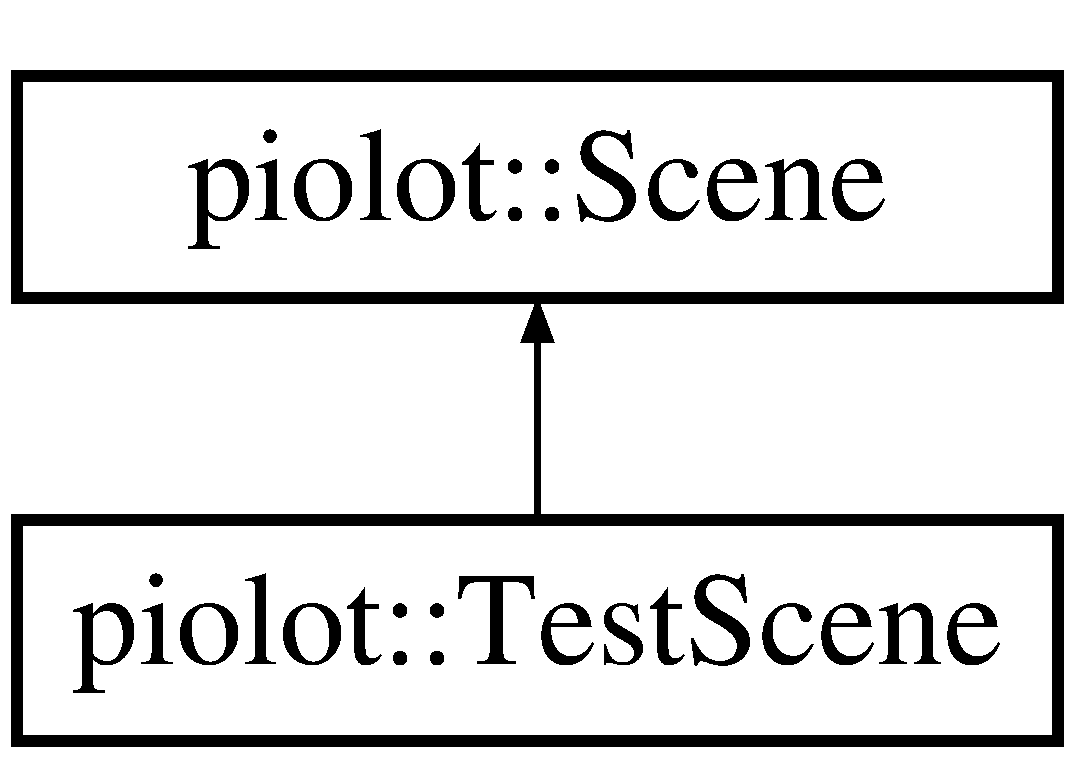
\includegraphics[height=2.000000cm]{classpiolot_1_1_scene}
\end{center}
\end{figure}
\subsection*{Public Member Functions}
\begin{DoxyCompactItemize}
\item 
\mbox{\hyperlink{classpiolot_1_1_scene_af42469b97e0c1006bec5d384223db148}{Scene}} (std\+::shared\+\_\+ptr$<$ \mbox{\hyperlink{class_window}{Window}} $>$ \+\_\+window)
\item 
virtual \mbox{\hyperlink{classpiolot_1_1_scene_aab1c2430f0f2317c0ae5b8fa8edc6fff}{$\sim$\+Scene}} ()=default
\item 
virtual void \mbox{\hyperlink{group___virtual_ga6871dbb3f61a724a166fd83c3c1dc3a3}{Init\+Entities}} ()=0
\begin{DoxyCompactList}\small\item\em Function to be overwritten to Initialize the Entities. \end{DoxyCompactList}\item 
virtual void \mbox{\hyperlink{group___virtual_gae05b812e9f1caa80526a79a03ab456e1}{On\+Update}} (float \+\_\+delta\+Time, float \+\_\+total\+Time)
\item 
virtual void \mbox{\hyperlink{group___virtual_gaaa3f6f2cb0dce355d890c8b43a2f11f2}{On\+Render}} ()=0
\item 
virtual void \mbox{\hyperlink{group___virtual_gaedea470f1c3485d76ef0681e4a503584}{On\+Imgui\+Render}} ()
\begin{DoxyCompactList}\small\item\em Render the Im\+G\+UI Stuff. \end{DoxyCompactList}\item 
void \mbox{\hyperlink{classpiolot_1_1_scene_a56d2c68922b38f97554ae4edde21f718}{Activate\+Camera}} (std\+::shared\+\_\+ptr$<$ \mbox{\hyperlink{classpiolot_1_1_camera}{Camera}} $>$ \+\_\+val)
\begin{DoxyCompactList}\small\item\em Activate the passed \mbox{\hyperlink{classpiolot_1_1_camera}{Camera}}. \end{DoxyCompactList}\item 
std\+::shared\+\_\+ptr$<$ \mbox{\hyperlink{classpiolot_1_1_camera}{Camera}} $>$ \mbox{\hyperlink{classpiolot_1_1_scene_ac0d71d1ad7c27872086d9f82ee7be7fb}{Get\+Active\+Camera}} () const
\begin{DoxyCompactList}\small\item\em Get the Active\+Camera. \end{DoxyCompactList}\end{DoxyCompactItemize}
\subsection*{Protected Attributes}
\begin{DoxyCompactItemize}
\item 
std\+::shared\+\_\+ptr$<$ \mbox{\hyperlink{class_window}{Window}} $>$ \mbox{\hyperlink{classpiolot_1_1_scene_a250749bf646c4ab0349bd98e515b0d5b}{window}}
\begin{DoxyCompactList}\small\item\em The Shared Pointer for the \mbox{\hyperlink{class_window}{Window}}. \end{DoxyCompactList}\item 
std\+::shared\+\_\+ptr$<$ \mbox{\hyperlink{classpiolot_1_1_camera}{Camera}} $>$ \mbox{\hyperlink{classpiolot_1_1_scene_a980ee452f49233f7b95fa4643e383ae9}{active\+Camera}}
\begin{DoxyCompactList}\small\item\em The \mbox{\hyperlink{classpiolot_1_1_camera}{Camera}} that is currently Active. \end{DoxyCompactList}\item 
std\+::unordered\+\_\+map$<$ std\+::string, std\+::shared\+\_\+ptr$<$ \mbox{\hyperlink{classpiolot_1_1_camera}{Camera}} $>$ $>$ \mbox{\hyperlink{classpiolot_1_1_scene_a03ce910c0242bb786e797d54bbffd54f}{cameras}}
\begin{DoxyCompactList}\small\item\em The Map of all the Cameras that are currently in the \mbox{\hyperlink{classpiolot_1_1_scene}{Scene}}. \end{DoxyCompactList}\item 
std\+::vector$<$ std\+::unique\+\_\+ptr$<$ \mbox{\hyperlink{classpiolot_1_1_entity}{Entity}} $>$ $>$ \mbox{\hyperlink{classpiolot_1_1_scene_ac85cd14260516aaaac3dacab4138a662}{entities}}
\begin{DoxyCompactList}\small\item\em All the Entities. \end{DoxyCompactList}\item 
std\+::vector$<$ std\+::unique\+\_\+ptr$<$ \mbox{\hyperlink{classpiolot_1_1_animated_entity}{Animated\+Entity}} $>$ $>$ \mbox{\hyperlink{classpiolot_1_1_scene_a6253e5cbedc67830e76d6da04c0b4371}{animated\+Entities}}
\begin{DoxyCompactList}\small\item\em All the Entities with Animations. \end{DoxyCompactList}\item 
std\+::vector$<$ \mbox{\hyperlink{classpiolot_1_1_entity}{Entity}} $\ast$ $>$ \mbox{\hyperlink{classpiolot_1_1_scene_a62abd7ccaa90a04e1f9738de7b2f96d3}{selected\+Entities}}
\begin{DoxyCompactList}\small\item\em Raw Pointers to the Selected Entities. \end{DoxyCompactList}\item 
std\+::vector$<$ std\+::unique\+\_\+ptr$<$ \mbox{\hyperlink{classpiolot_1_1_entity}{Entity}} $>$ $>$ \mbox{\hyperlink{classpiolot_1_1_scene_afb5dae5e574ec94da2b1192070e91327}{temp\+Entities}}
\begin{DoxyCompactList}\small\item\em Raw Pointers to the Temporary Entities. \end{DoxyCompactList}\item 
float \mbox{\hyperlink{classpiolot_1_1_scene_a10140d7b13ab259d8770d9cf44ab8829}{total\+Time}}
\begin{DoxyCompactList}\small\item\em Total time since the \mbox{\hyperlink{class_window}{Window}} Opened. \end{DoxyCompactList}\item 
float \mbox{\hyperlink{classpiolot_1_1_scene_ac3714002379b5e74cc24d947757f4af4}{delta\+Time}}
\begin{DoxyCompactList}\small\item\em The time elapsed since the last frame. \end{DoxyCompactList}\end{DoxyCompactItemize}


\subsection{Constructor \& Destructor Documentation}
\mbox{\Hypertarget{classpiolot_1_1_scene_af42469b97e0c1006bec5d384223db148}\label{classpiolot_1_1_scene_af42469b97e0c1006bec5d384223db148}} 
\index{piolot\+::\+Scene@{piolot\+::\+Scene}!Scene@{Scene}}
\index{Scene@{Scene}!piolot\+::\+Scene@{piolot\+::\+Scene}}
\subsubsection{\texorpdfstring{Scene()}{Scene()}}
{\footnotesize\ttfamily piolot\+::\+Scene\+::\+Scene (\begin{DoxyParamCaption}\item[{std\+::shared\+\_\+ptr$<$ \mbox{\hyperlink{class_window}{Window}} $>$}]{\+\_\+window }\end{DoxyParamCaption})\hspace{0.3cm}{\ttfamily [inline]}, {\ttfamily [explicit]}}

\mbox{\Hypertarget{classpiolot_1_1_scene_aab1c2430f0f2317c0ae5b8fa8edc6fff}\label{classpiolot_1_1_scene_aab1c2430f0f2317c0ae5b8fa8edc6fff}} 
\index{piolot\+::\+Scene@{piolot\+::\+Scene}!````~Scene@{$\sim$\+Scene}}
\index{````~Scene@{$\sim$\+Scene}!piolot\+::\+Scene@{piolot\+::\+Scene}}
\subsubsection{\texorpdfstring{$\sim$\+Scene()}{~Scene()}}
{\footnotesize\ttfamily virtual piolot\+::\+Scene\+::$\sim$\+Scene (\begin{DoxyParamCaption}{ }\end{DoxyParamCaption})\hspace{0.3cm}{\ttfamily [virtual]}, {\ttfamily [default]}}



\subsection{Member Function Documentation}
\mbox{\Hypertarget{classpiolot_1_1_scene_a56d2c68922b38f97554ae4edde21f718}\label{classpiolot_1_1_scene_a56d2c68922b38f97554ae4edde21f718}} 
\index{piolot\+::\+Scene@{piolot\+::\+Scene}!Activate\+Camera@{Activate\+Camera}}
\index{Activate\+Camera@{Activate\+Camera}!piolot\+::\+Scene@{piolot\+::\+Scene}}
\subsubsection{\texorpdfstring{Activate\+Camera()}{ActivateCamera()}}
{\footnotesize\ttfamily void piolot\+::\+Scene\+::\+Activate\+Camera (\begin{DoxyParamCaption}\item[{std\+::shared\+\_\+ptr$<$ \mbox{\hyperlink{classpiolot_1_1_camera}{Camera}} $>$}]{\+\_\+val }\end{DoxyParamCaption})\hspace{0.3cm}{\ttfamily [inline]}}



Activate the passed \mbox{\hyperlink{classpiolot_1_1_camera}{Camera}}. 


\begin{DoxyParams}{Parameters}
{\em val} & The \mbox{\hyperlink{classpiolot_1_1_camera}{Camera}} to Activate \\
\hline
\end{DoxyParams}
\mbox{\Hypertarget{classpiolot_1_1_scene_ac0d71d1ad7c27872086d9f82ee7be7fb}\label{classpiolot_1_1_scene_ac0d71d1ad7c27872086d9f82ee7be7fb}} 
\index{piolot\+::\+Scene@{piolot\+::\+Scene}!Get\+Active\+Camera@{Get\+Active\+Camera}}
\index{Get\+Active\+Camera@{Get\+Active\+Camera}!piolot\+::\+Scene@{piolot\+::\+Scene}}
\subsubsection{\texorpdfstring{Get\+Active\+Camera()}{GetActiveCamera()}}
{\footnotesize\ttfamily std\+::shared\+\_\+ptr$<$\mbox{\hyperlink{classpiolot_1_1_camera}{Camera}}$>$ piolot\+::\+Scene\+::\+Get\+Active\+Camera (\begin{DoxyParamCaption}{ }\end{DoxyParamCaption}) const\hspace{0.3cm}{\ttfamily [inline]}}



Get the Active\+Camera. 

\begin{DoxyReturn}{Returns}
Returns a pointer to the Current Active \mbox{\hyperlink{classpiolot_1_1_camera}{Camera}} 
\end{DoxyReturn}


\subsection{Member Data Documentation}
\mbox{\Hypertarget{classpiolot_1_1_scene_a980ee452f49233f7b95fa4643e383ae9}\label{classpiolot_1_1_scene_a980ee452f49233f7b95fa4643e383ae9}} 
\index{piolot\+::\+Scene@{piolot\+::\+Scene}!active\+Camera@{active\+Camera}}
\index{active\+Camera@{active\+Camera}!piolot\+::\+Scene@{piolot\+::\+Scene}}
\subsubsection{\texorpdfstring{active\+Camera}{activeCamera}}
{\footnotesize\ttfamily std\+::shared\+\_\+ptr$<$\mbox{\hyperlink{classpiolot_1_1_camera}{Camera}}$>$ piolot\+::\+Scene\+::active\+Camera\hspace{0.3cm}{\ttfamily [protected]}}



The \mbox{\hyperlink{classpiolot_1_1_camera}{Camera}} that is currently Active. 

\mbox{\Hypertarget{classpiolot_1_1_scene_a6253e5cbedc67830e76d6da04c0b4371}\label{classpiolot_1_1_scene_a6253e5cbedc67830e76d6da04c0b4371}} 
\index{piolot\+::\+Scene@{piolot\+::\+Scene}!animated\+Entities@{animated\+Entities}}
\index{animated\+Entities@{animated\+Entities}!piolot\+::\+Scene@{piolot\+::\+Scene}}
\subsubsection{\texorpdfstring{animated\+Entities}{animatedEntities}}
{\footnotesize\ttfamily std\+::vector$<$std\+::unique\+\_\+ptr$<$\mbox{\hyperlink{classpiolot_1_1_animated_entity}{Animated\+Entity}}$>$ $>$ piolot\+::\+Scene\+::animated\+Entities\hspace{0.3cm}{\ttfamily [protected]}}



All the Entities with Animations. 

The \mbox{\hyperlink{classpiolot_1_1_scene}{Scene}} owns them. When you delete the \mbox{\hyperlink{classpiolot_1_1_scene}{Scene}}, the entities are deleted. \mbox{\Hypertarget{classpiolot_1_1_scene_a03ce910c0242bb786e797d54bbffd54f}\label{classpiolot_1_1_scene_a03ce910c0242bb786e797d54bbffd54f}} 
\index{piolot\+::\+Scene@{piolot\+::\+Scene}!cameras@{cameras}}
\index{cameras@{cameras}!piolot\+::\+Scene@{piolot\+::\+Scene}}
\subsubsection{\texorpdfstring{cameras}{cameras}}
{\footnotesize\ttfamily std\+::unordered\+\_\+map$<$std\+::string, std\+::shared\+\_\+ptr$<$\mbox{\hyperlink{classpiolot_1_1_camera}{Camera}}$>$ $>$ piolot\+::\+Scene\+::cameras\hspace{0.3cm}{\ttfamily [protected]}}



The Map of all the Cameras that are currently in the \mbox{\hyperlink{classpiolot_1_1_scene}{Scene}}. 

We use Unordered Map because when we disable the UI, we have a slight performance benefit for the Un\+Ordered Map. This is definitely worse when you have the UI Enabled. \mbox{\Hypertarget{classpiolot_1_1_scene_ac3714002379b5e74cc24d947757f4af4}\label{classpiolot_1_1_scene_ac3714002379b5e74cc24d947757f4af4}} 
\index{piolot\+::\+Scene@{piolot\+::\+Scene}!delta\+Time@{delta\+Time}}
\index{delta\+Time@{delta\+Time}!piolot\+::\+Scene@{piolot\+::\+Scene}}
\subsubsection{\texorpdfstring{delta\+Time}{deltaTime}}
{\footnotesize\ttfamily float piolot\+::\+Scene\+::delta\+Time\hspace{0.3cm}{\ttfamily [protected]}}



The time elapsed since the last frame. 

\mbox{\Hypertarget{classpiolot_1_1_scene_ac85cd14260516aaaac3dacab4138a662}\label{classpiolot_1_1_scene_ac85cd14260516aaaac3dacab4138a662}} 
\index{piolot\+::\+Scene@{piolot\+::\+Scene}!entities@{entities}}
\index{entities@{entities}!piolot\+::\+Scene@{piolot\+::\+Scene}}
\subsubsection{\texorpdfstring{entities}{entities}}
{\footnotesize\ttfamily std\+::vector$<$std\+::unique\+\_\+ptr$<$\mbox{\hyperlink{classpiolot_1_1_entity}{Entity}}$>$ $>$ piolot\+::\+Scene\+::entities\hspace{0.3cm}{\ttfamily [protected]}}



All the Entities. 

The \mbox{\hyperlink{classpiolot_1_1_scene}{Scene}} owns them. When you delete the \mbox{\hyperlink{classpiolot_1_1_scene}{Scene}}, the entities are deleted. \mbox{\Hypertarget{classpiolot_1_1_scene_a62abd7ccaa90a04e1f9738de7b2f96d3}\label{classpiolot_1_1_scene_a62abd7ccaa90a04e1f9738de7b2f96d3}} 
\index{piolot\+::\+Scene@{piolot\+::\+Scene}!selected\+Entities@{selected\+Entities}}
\index{selected\+Entities@{selected\+Entities}!piolot\+::\+Scene@{piolot\+::\+Scene}}
\subsubsection{\texorpdfstring{selected\+Entities}{selectedEntities}}
{\footnotesize\ttfamily std\+::vector$<$\mbox{\hyperlink{classpiolot_1_1_entity}{Entity}} $\ast$$>$ piolot\+::\+Scene\+::selected\+Entities\hspace{0.3cm}{\ttfamily [protected]}}



Raw Pointers to the Selected Entities. 

These selected entities can be destroyed even though they are selected. So, we just copy the addresses. \mbox{\Hypertarget{classpiolot_1_1_scene_afb5dae5e574ec94da2b1192070e91327}\label{classpiolot_1_1_scene_afb5dae5e574ec94da2b1192070e91327}} 
\index{piolot\+::\+Scene@{piolot\+::\+Scene}!temp\+Entities@{temp\+Entities}}
\index{temp\+Entities@{temp\+Entities}!piolot\+::\+Scene@{piolot\+::\+Scene}}
\subsubsection{\texorpdfstring{temp\+Entities}{tempEntities}}
{\footnotesize\ttfamily std\+::vector$<$std\+::unique\+\_\+ptr$<$\mbox{\hyperlink{classpiolot_1_1_entity}{Entity}}$>$ $>$ piolot\+::\+Scene\+::temp\+Entities\hspace{0.3cm}{\ttfamily [protected]}}



Raw Pointers to the Temporary Entities. 

These entities are cleared every frame, after they are drawn. \mbox{\Hypertarget{classpiolot_1_1_scene_a10140d7b13ab259d8770d9cf44ab8829}\label{classpiolot_1_1_scene_a10140d7b13ab259d8770d9cf44ab8829}} 
\index{piolot\+::\+Scene@{piolot\+::\+Scene}!total\+Time@{total\+Time}}
\index{total\+Time@{total\+Time}!piolot\+::\+Scene@{piolot\+::\+Scene}}
\subsubsection{\texorpdfstring{total\+Time}{totalTime}}
{\footnotesize\ttfamily float piolot\+::\+Scene\+::total\+Time\hspace{0.3cm}{\ttfamily [protected]}}



Total time since the \mbox{\hyperlink{class_window}{Window}} Opened. 

Populated by using glfwgettime() function. \begin{DoxySeeAlso}{See also}
\href{https://www.glfw.org/docs/3.0/group__time.html}{\tt https\+://www.\+glfw.\+org/docs/3.\+0/group\+\_\+\+\_\+time.\+html} 
\end{DoxySeeAlso}
\mbox{\Hypertarget{classpiolot_1_1_scene_a250749bf646c4ab0349bd98e515b0d5b}\label{classpiolot_1_1_scene_a250749bf646c4ab0349bd98e515b0d5b}} 
\index{piolot\+::\+Scene@{piolot\+::\+Scene}!window@{window}}
\index{window@{window}!piolot\+::\+Scene@{piolot\+::\+Scene}}
\subsubsection{\texorpdfstring{window}{window}}
{\footnotesize\ttfamily std\+::shared\+\_\+ptr$<$\mbox{\hyperlink{class_window}{Window}}$>$ piolot\+::\+Scene\+::window\hspace{0.3cm}{\ttfamily [protected]}}



The Shared Pointer for the \mbox{\hyperlink{class_window}{Window}}. 



The documentation for this class was generated from the following file\+:\begin{DoxyCompactItemize}
\item 
\mbox{\hyperlink{_scene_8h}{Scene.\+h}}\end{DoxyCompactItemize}

\hypertarget{classpiolot_1_1_terrain}{}\section{piolot\+:\+:Terrain Class Reference}
\label{classpiolot_1_1_terrain}\index{piolot\+::\+Terrain@{piolot\+::\+Terrain}}
Inheritance diagram for piolot\+:\+:Terrain\+:\begin{figure}[H]
\begin{center}
\leavevmode
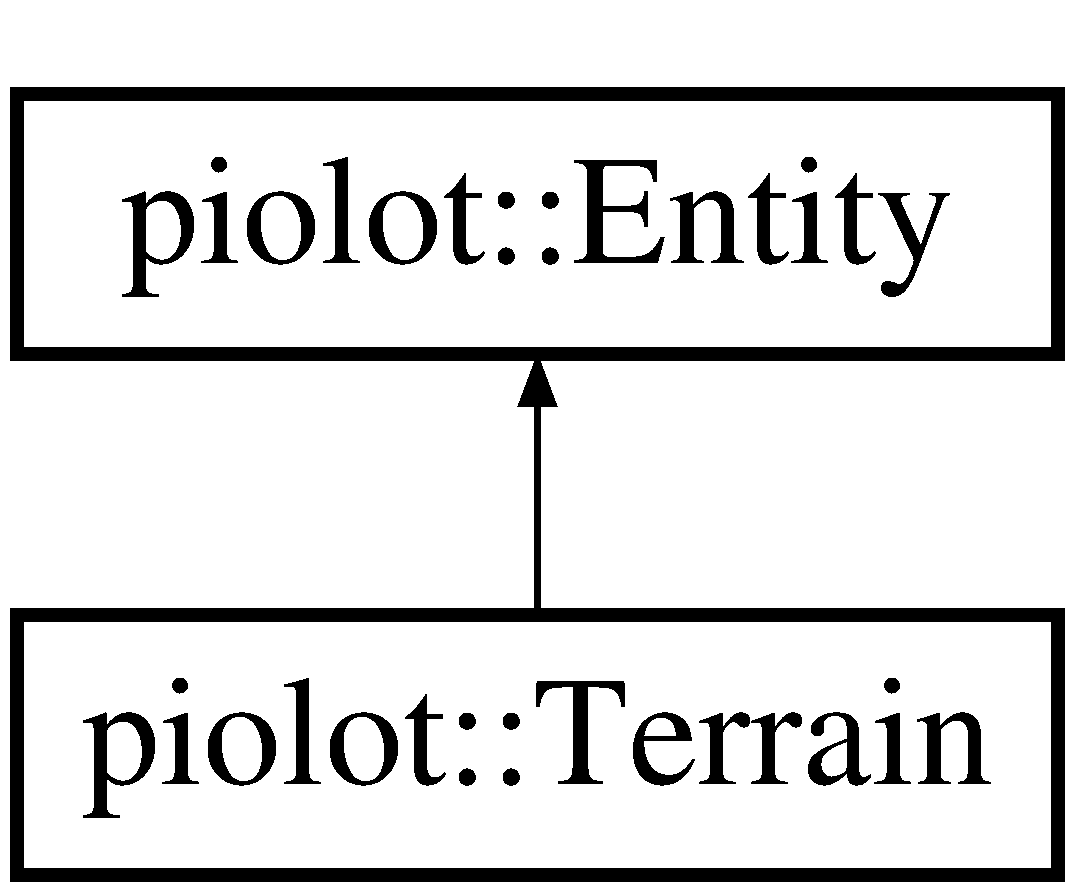
\includegraphics[height=2.000000cm]{classpiolot_1_1_terrain}
\end{center}
\end{figure}
\subsection*{Public Member Functions}
\begin{DoxyCompactItemize}
\item 
\mbox{\Hypertarget{classpiolot_1_1_terrain_aeb2f5954d70bc27d7dc84ab15180c502}\label{classpiolot_1_1_terrain_aeb2f5954d70bc27d7dc84ab15180c502}} 
unsigned {\bfseries Get\+Length} () const
\item 
\mbox{\Hypertarget{classpiolot_1_1_terrain_a7fa4bf450e2545dbce46a870caa31aa2}\label{classpiolot_1_1_terrain_a7fa4bf450e2545dbce46a870caa31aa2}} 
unsigned {\bfseries Get\+Breadth} () const
\item 
\mbox{\Hypertarget{classpiolot_1_1_terrain_aa742fdf411184356e962f98d3785ec7c}\label{classpiolot_1_1_terrain_aa742fdf411184356e962f98d3785ec7c}} 
float {\bfseries Get\+Grid\+Length} () const
\item 
\mbox{\Hypertarget{classpiolot_1_1_terrain_acd20433446ca1eef57b1498e26aa0aca}\label{classpiolot_1_1_terrain_acd20433446ca1eef57b1498e26aa0aca}} 
float {\bfseries Get\+Grid\+Breadth} () const
\item 
\mbox{\Hypertarget{classpiolot_1_1_terrain_a284fb2b373798b73d3893837cfe5d4bc}\label{classpiolot_1_1_terrain_a284fb2b373798b73d3893837cfe5d4bc}} 
unsigned {\bfseries Get\+Node\+CountX} () const
\item 
\mbox{\Hypertarget{classpiolot_1_1_terrain_aef96f5a95563a88c641fbfd299c905f3}\label{classpiolot_1_1_terrain_aef96f5a95563a88c641fbfd299c905f3}} 
unsigned {\bfseries Get\+Node\+CountZ} () const
\item 
\mbox{\Hypertarget{classpiolot_1_1_terrain_a0366991939da62e46bff441c1b3988e0}\label{classpiolot_1_1_terrain_a0366991939da62e46bff441c1b3988e0}} 
\mbox{\hyperlink{classpiolot_1_1_map_tile}{Map\+Tile}} $\ast$$\ast$ {\bfseries Get\+Tiles} () const
\item 
\mbox{\Hypertarget{classpiolot_1_1_terrain_a8ce0f148b1b05889f609796d09840543}\label{classpiolot_1_1_terrain_a8ce0f148b1b05889f609796d09840543}} 
const std\+::string \& {\bfseries Get\+Height\+Map\+File} () const
\item 
\mbox{\Hypertarget{classpiolot_1_1_terrain_a0fe5987e17e76c418cc9407a1acdc915}\label{classpiolot_1_1_terrain_a0fe5987e17e76c418cc9407a1acdc915}} 
const std\+::vector$<$ \mbox{\hyperlink{structpiolot_1_1_terrain_vertex_data}{Terrain\+Vertex\+Data}} $>$ \& {\bfseries Get\+Vertices} () const
\item 
\mbox{\Hypertarget{classpiolot_1_1_terrain_ada8caf451e4946153d9a0cc4d5d0fcaf}\label{classpiolot_1_1_terrain_ada8caf451e4946153d9a0cc4d5d0fcaf}} 
const std\+::vector$<$ unsigned $>$ \& {\bfseries Get\+Indices} () const
\item 
\mbox{\Hypertarget{classpiolot_1_1_terrain_a445ca2537de1765c3ae2c8073db1603f}\label{classpiolot_1_1_terrain_a445ca2537de1765c3ae2c8073db1603f}} 
const std\+::shared\+\_\+ptr$<$ \mbox{\hyperlink{classpiolot_1_1_object}{Object}} $>$ \& {\bfseries Get\+Object\+Ptr} () const
\item 
\mbox{\Hypertarget{classpiolot_1_1_terrain_aa60d6ba8d6dd4affb441d15eda4ca0f8}\label{classpiolot_1_1_terrain_aa60d6ba8d6dd4affb441d15eda4ca0f8}} 
{\bfseries Terrain} (int \+\_\+map\+Length, int \+\_\+map\+Breadth, float \+\_\+grid\+Length, float \+\_\+grid\+Breadth, std\+::string \+\_\+height\+Map\+File)
\item 
\mbox{\Hypertarget{classpiolot_1_1_terrain_af737ba0aa165e923a3e6bd37f6c9a9ab}\label{classpiolot_1_1_terrain_af737ba0aa165e923a3e6bd37f6c9a9ab}} 
void {\bfseries Init} ()
\item 
\mbox{\Hypertarget{classpiolot_1_1_terrain_a21bf8a5f9f394709f2e938bf2a62db9c}\label{classpiolot_1_1_terrain_a21bf8a5f9f394709f2e938bf2a62db9c}} 
void {\bfseries Render} ()
\item 
\mbox{\Hypertarget{classpiolot_1_1_terrain_a54f2eb43b93352f7584569f15a7dc824}\label{classpiolot_1_1_terrain_a54f2eb43b93352f7584569f15a7dc824}} 
void {\bfseries Update} (float \+\_\+delat\+Time, float \+\_\+total\+Time)
\item 
\mbox{\Hypertarget{classpiolot_1_1_terrain_a8eb74a9d2b2c403ff454dc639b47fcdd}\label{classpiolot_1_1_terrain_a8eb74a9d2b2c403ff454dc639b47fcdd}} 
float {\bfseries Get\+Height\+At\+Pos} (const float \&\+\_\+x, const float \&\+\_\+z)
\item 
\mbox{\Hypertarget{classpiolot_1_1_terrain_ab34c88011a034755e5758985b9e02cc6}\label{classpiolot_1_1_terrain_ab34c88011a034755e5758985b9e02cc6}} 
float {\bfseries Get\+Height\+For\+Node} (const int \&\+\_\+x, const int \&\+\_\+z)
\item 
\mbox{\Hypertarget{classpiolot_1_1_terrain_a8ac0b5aef5986ea7c78d645742a6b51a}\label{classpiolot_1_1_terrain_a8ac0b5aef5986ea7c78d645742a6b51a}} 
glm\+::vec2 {\bfseries Get\+Node\+Indices\+From\+Pos} (const float \&\+\_\+x, const float \&\+\_\+z) const
\item 
\mbox{\Hypertarget{classpiolot_1_1_terrain_af9a39ab31e9621d02f78d89518c521f7}\label{classpiolot_1_1_terrain_af9a39ab31e9621d02f78d89518c521f7}} 
void {\bfseries Highlight\+Node} (const unsigned int \+\_\+x, const unsigned int \+\_\+z)
\item 
\mbox{\Hypertarget{classpiolot_1_1_terrain_afe488b112444dc406a12fe83f8fb1a90}\label{classpiolot_1_1_terrain_afe488b112444dc406a12fe83f8fb1a90}} 
void {\bfseries Clear\+Colours} ()
\item 
\mbox{\Hypertarget{classpiolot_1_1_terrain_af3294a6025d6e23f79ff8693ca67fb79}\label{classpiolot_1_1_terrain_af3294a6025d6e23f79ff8693ca67fb79}} 
std\+::vector$<$ \mbox{\hyperlink{classpiolot_1_1_map_tile}{Map\+Tile}} $\ast$ $>$ {\bfseries Get\+Path\+From\+Tiles} (\mbox{\hyperlink{classpiolot_1_1_map_tile}{Map\+Tile}} $\ast$\+\_\+start\+Tile, \mbox{\hyperlink{classpiolot_1_1_map_tile}{Map\+Tile}} $\ast$\+\_\+end\+Tile)
\item 
\mbox{\Hypertarget{classpiolot_1_1_terrain_a27ab93eb2d5e058f4bfa9e6929b324bc}\label{classpiolot_1_1_terrain_a27ab93eb2d5e058f4bfa9e6929b324bc}} 
std\+::vector$<$ \mbox{\hyperlink{classpiolot_1_1_map_tile}{Map\+Tile}} $\ast$ $>$ {\bfseries Get\+Path\+From\+Positions} (glm\+::vec3, glm\+::vec3)
\item 
\mbox{\Hypertarget{classpiolot_1_1_terrain_a1dde3530579a5bcdbb35eec94dff49b5}\label{classpiolot_1_1_terrain_a1dde3530579a5bcdbb35eec94dff49b5}} 
\mbox{\hyperlink{classpiolot_1_1_map_tile}{Map\+Tile}} $\ast$ {\bfseries Get\+Tile\+From\+Indices} (int \+\_\+x, int \+\_\+y)
\item 
\mbox{\Hypertarget{classpiolot_1_1_terrain_a8c86b33ae5763a67ad783bebb37d88c5}\label{classpiolot_1_1_terrain_a8c86b33ae5763a67ad783bebb37d88c5}} 
void {\bfseries Init\+Path\+Finding} ()
\item 
\mbox{\Hypertarget{classpiolot_1_1_terrain_ae61a150d060f54eb14ef465541cc6214}\label{classpiolot_1_1_terrain_ae61a150d060f54eb14ef465541cc6214}} 
void {\bfseries Fill\+Neighbours} (\mbox{\hyperlink{classpiolot_1_1_map_tile}{Map\+Tile}} \&\+\_\+tile)
\item 
\mbox{\Hypertarget{classpiolot_1_1_terrain_a211e06f07b056d9e412f9b7d5c61f28f}\label{classpiolot_1_1_terrain_a211e06f07b056d9e412f9b7d5c61f28f}} 
void {\bfseries On\+Imgui\+Render} ()
\item 
\mbox{\Hypertarget{classpiolot_1_1_terrain_a653f471121e6efec6fc9533e747486ae}\label{classpiolot_1_1_terrain_a653f471121e6efec6fc9533e747486ae}} 
int {\bfseries Get\+Node\+Set\+From\+Pos} (float \+\_\+x, float \+\_\+z)
\item 
\mbox{\Hypertarget{classpiolot_1_1_terrain_a1008afdeef49245b34551141ad40e512}\label{classpiolot_1_1_terrain_a1008afdeef49245b34551141ad40e512}} 
std\+::vector$<$ int $>$ {\bfseries Get\+All\+Tile\+Sets} ()
\item 
\mbox{\Hypertarget{classpiolot_1_1_terrain_a2a3fee4479a1c367262917e87e80aeae}\label{classpiolot_1_1_terrain_a2a3fee4479a1c367262917e87e80aeae}} 
void {\bfseries Save\+To\+File} (std\+::ofstream \&\+\_\+out)
\item 
\mbox{\Hypertarget{classpiolot_1_1_terrain_ab975d5914a10346ddcbe29467f0862c2}\label{classpiolot_1_1_terrain_ab975d5914a10346ddcbe29467f0862c2}} 
void {\bfseries Load\+From\+File} (std\+::ifstream \&\+\_\+in)
\item 
\mbox{\Hypertarget{classpiolot_1_1_terrain_af2bc3eb0ea909a0fd96b6c11aeb29c8a}\label{classpiolot_1_1_terrain_af2bc3eb0ea909a0fd96b6c11aeb29c8a}} 
void {\bfseries Delete\+Tiles} () const
\end{DoxyCompactItemize}
\subsection*{Public Attributes}
\begin{DoxyCompactItemize}
\item 
\mbox{\Hypertarget{classpiolot_1_1_terrain_af15b6de452d8225d07d7d4ae48d4f154}\label{classpiolot_1_1_terrain_af15b6de452d8225d07d7d4ae48d4f154}} 
bool {\bfseries terrain\+Debug} = false
\end{DoxyCompactItemize}
\subsection*{Private Member Functions}
\begin{DoxyCompactItemize}
\item 
\mbox{\Hypertarget{classpiolot_1_1_terrain_a8228070fe11ba581ee8a8b8f9fe303d4}\label{classpiolot_1_1_terrain_a8228070fe11ba581ee8a8b8f9fe303d4}} 
glm\+::vec3 {\bfseries Compute\+Grid\+Normal} (int \+\_\+x, int \+\_\+z)
\end{DoxyCompactItemize}
\subsection*{Private Attributes}
\begin{DoxyCompactItemize}
\item 
\mbox{\Hypertarget{classpiolot_1_1_terrain_adfe24e50e102f6c0dd424e2e7f376f15}\label{classpiolot_1_1_terrain_adfe24e50e102f6c0dd424e2e7f376f15}} 
unsigned int {\bfseries length}
\item 
\mbox{\Hypertarget{classpiolot_1_1_terrain_a05c6d7e235fafccc8aaa300fb63dfc27}\label{classpiolot_1_1_terrain_a05c6d7e235fafccc8aaa300fb63dfc27}} 
unsigned int {\bfseries breadth}
\item 
\mbox{\Hypertarget{classpiolot_1_1_terrain_ac1378a19d70d35bcafa1ac2c9e443d98}\label{classpiolot_1_1_terrain_ac1378a19d70d35bcafa1ac2c9e443d98}} 
float {\bfseries grid\+Length}
\item 
\mbox{\Hypertarget{classpiolot_1_1_terrain_ac825eeb29fe45a95909488a560ac8331}\label{classpiolot_1_1_terrain_ac825eeb29fe45a95909488a560ac8331}} 
float {\bfseries grid\+Breadth}
\item 
\mbox{\Hypertarget{classpiolot_1_1_terrain_af2671f954c4fa1be2228ccf4cb631abf}\label{classpiolot_1_1_terrain_af2671f954c4fa1be2228ccf4cb631abf}} 
unsigned int {\bfseries node\+CountX} \{\}
\item 
\mbox{\Hypertarget{classpiolot_1_1_terrain_a584b5d99c115bcfae303b3feea50c3a5}\label{classpiolot_1_1_terrain_a584b5d99c115bcfae303b3feea50c3a5}} 
unsigned int {\bfseries node\+CountZ} \{\}
\item 
\mbox{\Hypertarget{classpiolot_1_1_terrain_a092c31b5d881c4f89dac30cd887d1664}\label{classpiolot_1_1_terrain_a092c31b5d881c4f89dac30cd887d1664}} 
\mbox{\hyperlink{classpiolot_1_1_map_tile}{Map\+Tile}} $\ast$$\ast$ {\bfseries tiles} \{\}
\item 
\mbox{\Hypertarget{classpiolot_1_1_terrain_a75cfcac6fb95fb3c63def8362ce393d0}\label{classpiolot_1_1_terrain_a75cfcac6fb95fb3c63def8362ce393d0}} 
std\+::string {\bfseries height\+Map\+File}
\item 
\mbox{\Hypertarget{classpiolot_1_1_terrain_a57bd2f1b451a1d670bc5f42134ecf2c0}\label{classpiolot_1_1_terrain_a57bd2f1b451a1d670bc5f42134ecf2c0}} 
std\+::vector$<$ \mbox{\hyperlink{structpiolot_1_1_terrain_vertex_data}{Terrain\+Vertex\+Data}} $>$ {\bfseries vertices}
\item 
\mbox{\Hypertarget{classpiolot_1_1_terrain_a0d8413db780f4ef041fd1794631ef122}\label{classpiolot_1_1_terrain_a0d8413db780f4ef041fd1794631ef122}} 
bool {\bfseries are\+Vertices\+Dirty} = false
\item 
\mbox{\Hypertarget{classpiolot_1_1_terrain_a3f6ce2a18736eccd598931c72aeaf4bc}\label{classpiolot_1_1_terrain_a3f6ce2a18736eccd598931c72aeaf4bc}} 
std\+::vector$<$ unsigned int $>$ {\bfseries indices}
\item 
\mbox{\Hypertarget{classpiolot_1_1_terrain_a9711e78acb58e6d457758fc1ddd8d82d}\label{classpiolot_1_1_terrain_a9711e78acb58e6d457758fc1ddd8d82d}} 
std\+::shared\+\_\+ptr$<$ \mbox{\hyperlink{classpiolot_1_1_object}{Object}} $>$ {\bfseries object\+Ptr}
\item 
\mbox{\Hypertarget{classpiolot_1_1_terrain_aa658452ff45b3c472d7f8290ee689954}\label{classpiolot_1_1_terrain_aa658452ff45b3c472d7f8290ee689954}} 
glm\+::vec2 {\bfseries startxz} \{\}
\item 
\mbox{\Hypertarget{classpiolot_1_1_terrain_abef2d354599b2fa104c4aa0c62035257}\label{classpiolot_1_1_terrain_abef2d354599b2fa104c4aa0c62035257}} 
glm\+::vec2 {\bfseries endxz} \{\}
\end{DoxyCompactItemize}
\subsection*{Additional Inherited Members}


The documentation for this class was generated from the following files\+:\begin{DoxyCompactItemize}
\item 
C\+:/dev/\+Piolot/\+Engine/Terrain.\+h\item 
C\+:/dev/\+Piolot/\+Engine/Terrain.\+cpp\end{DoxyCompactItemize}

\hypertarget{structpiolot_1_1_terrain_vertex_data}{}\section{piolot\+:\+:Terrain\+Vertex\+Data Struct Reference}
\label{structpiolot_1_1_terrain_vertex_data}\index{piolot\+::\+Terrain\+Vertex\+Data@{piolot\+::\+Terrain\+Vertex\+Data}}
\subsection*{Public Attributes}
\begin{DoxyCompactItemize}
\item 
\mbox{\Hypertarget{structpiolot_1_1_terrain_vertex_data_a7a00a745d0492b03adf53487960a2469}\label{structpiolot_1_1_terrain_vertex_data_a7a00a745d0492b03adf53487960a2469}} 
glm\+::vec3 {\bfseries position}
\item 
\mbox{\Hypertarget{structpiolot_1_1_terrain_vertex_data_a61e13493d45cce67d98e5c9d54bbe2ec}\label{structpiolot_1_1_terrain_vertex_data_a61e13493d45cce67d98e5c9d54bbe2ec}} 
glm\+::vec3 {\bfseries normal}
\item 
\mbox{\Hypertarget{structpiolot_1_1_terrain_vertex_data_ac739ba374cf5a2e06af669c20754f143}\label{structpiolot_1_1_terrain_vertex_data_ac739ba374cf5a2e06af669c20754f143}} 
glm\+::vec3 {\bfseries colour}
\item 
\mbox{\Hypertarget{structpiolot_1_1_terrain_vertex_data_ab18681a402838040b7ceb7574921e472}\label{structpiolot_1_1_terrain_vertex_data_ab18681a402838040b7ceb7574921e472}} 
glm\+::vec3 {\bfseries tex\+Coord}
\end{DoxyCompactItemize}


The documentation for this struct was generated from the following file\+:\begin{DoxyCompactItemize}
\item 
C\+:/dev/\+Piolot/\+Engine/Terrain.\+h\end{DoxyCompactItemize}

\hypertarget{classpiolot_1_1_test_scene}{}\section{piolot\+:\+:Test\+Scene Class Reference}
\label{classpiolot_1_1_test_scene}\index{piolot\+::\+Test\+Scene@{piolot\+::\+Test\+Scene}}


{\ttfamily \#include $<$Test\+Scene.\+h$>$}

Inheritance diagram for piolot\+:\+:Test\+Scene\+:\begin{figure}[H]
\begin{center}
\leavevmode
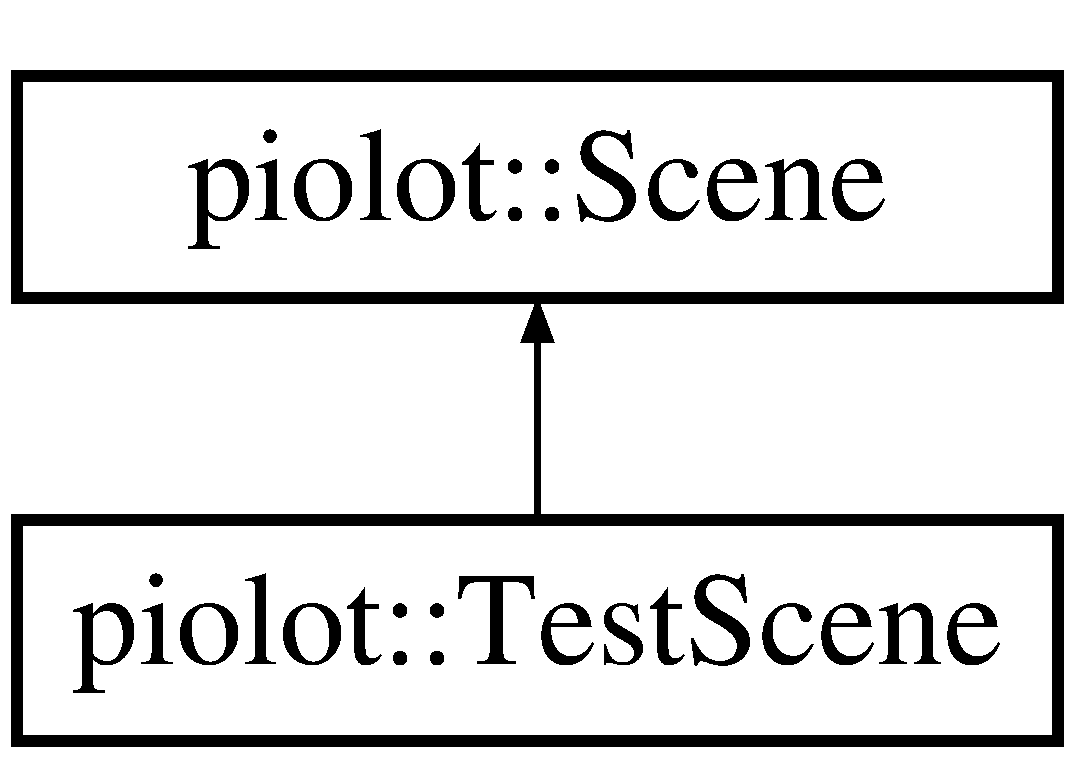
\includegraphics[height=2.000000cm]{classpiolot_1_1_test_scene}
\end{center}
\end{figure}
\subsection*{Public Member Functions}
\begin{DoxyCompactItemize}
\item 
\mbox{\hyperlink{classpiolot_1_1_test_scene_a1568f961f1632ccb9da36d14c6aae0d5}{Test\+Scene}} (std\+::shared\+\_\+ptr$<$ \mbox{\hyperlink{class_window}{Window}} $>$ \+\_\+window)
\item 
\mbox{\hyperlink{classpiolot_1_1_test_scene_a615e7e4264391f122ffdf0f997c825f4}{$\sim$\+Test\+Scene}} ()=default
\item 
void \mbox{\hyperlink{classpiolot_1_1_test_scene_a76c03545ecd764cd4350eec338c9a94e}{Init\+Entities}} () override
\begin{DoxyCompactList}\small\item\em Initialize all the Entities that shall be present in the \mbox{\hyperlink{classpiolot_1_1_scene}{Scene}} when it loads. \end{DoxyCompactList}\item 
void \mbox{\hyperlink{classpiolot_1_1_test_scene_a1151c075257a2b626774502709e0aab9}{On\+Update}} (float \+\_\+delta\+Time, float \+\_\+total\+Time) override
\begin{DoxyCompactList}\small\item\em Update the program by one frame. \end{DoxyCompactList}\item 
void \mbox{\hyperlink{classpiolot_1_1_test_scene_aeaccbb83f264fb4f1e8df5b246033f76}{On\+Render}} () override
\begin{DoxyCompactList}\small\item\em Render the \mbox{\hyperlink{classpiolot_1_1_scene}{Scene}}. \end{DoxyCompactList}\item 
virtual void \mbox{\hyperlink{classpiolot_1_1_test_scene_aa75a09c9c598fc35949f097cbb6df5cb}{On\+Imgui\+Render}} (\mbox{\hyperlink{structpiolot_1_1_im_gui_control_variables}{Im\+Gui\+Control\+Variables}} \&\+\_\+vars)
\begin{DoxyCompactList}\small\item\em Render the Im\+G\+UI\textquotesingle{}s current Frame. \end{DoxyCompactList}\item 
void \mbox{\hyperlink{classpiolot_1_1_test_scene_a8fcd4f46ccdb6c49741bb37364d9bb0e}{Save\+Scene}} (const char $\ast$\+\_\+file\+Name)
\begin{DoxyCompactList}\small\item\em Save the current \mbox{\hyperlink{classpiolot_1_1_scene}{Scene}} to a binary file. \end{DoxyCompactList}\item 
void \mbox{\hyperlink{classpiolot_1_1_test_scene_a513072b5c63768aa0fcd0dd5a0a0ca98}{Load\+Scene}} (const char $\ast$\+\_\+file\+Name)
\begin{DoxyCompactList}\small\item\em Load the \mbox{\hyperlink{classpiolot_1_1_scene}{Scene}} from the binary file. \end{DoxyCompactList}\item 
void \mbox{\hyperlink{classpiolot_1_1_test_scene_a22c630a5e1c5725f04140ec15a125de7}{Ray\+Picking}} ()
\end{DoxyCompactItemize}
\subsection*{Private Attributes}
\begin{DoxyCompactItemize}
\item 
\mbox{\hyperlink{classpiolot_1_1_grid}{Grid}} \mbox{\hyperlink{classpiolot_1_1_test_scene_aca94d51dc521dd620b45d85ee817cb0a}{test\+Grid}}
\item 
std\+::shared\+\_\+ptr$<$ \mbox{\hyperlink{classpiolot_1_1_terrain}{Terrain}} $>$ \mbox{\hyperlink{classpiolot_1_1_test_scene_a349626f35bec9409fa359108ce08c32e}{test\+Terrain}}
\item 
std\+::unique\+\_\+ptr$<$ \mbox{\hyperlink{classpiolot_1_1_entity}{Entity}} $>$ \mbox{\hyperlink{classpiolot_1_1_test_scene_ae0a460b8b6b3d352f92be069a6d69fb3}{building\+Placer}}
\begin{DoxyCompactList}\small\item\em This would be a temporary entity that we draw when we are in the Placing Mode. \end{DoxyCompactList}\item 
glm\+::vec2 \mbox{\hyperlink{classpiolot_1_1_test_scene_ab19142067d70aede9c5ac3cadecb1c29}{startxz}}
\item 
glm\+::vec2 \mbox{\hyperlink{classpiolot_1_1_test_scene_aa7838a55b521b6d9c1d32dc3ca240ba7}{endxz}}
\item 
float \mbox{\hyperlink{classpiolot_1_1_test_scene_ad676a1a351b61b8e7071b2d91856ad14}{total\+Time\+Counter\+For\+Pathing}} = 0
\item 
std\+::vector$<$ \mbox{\hyperlink{classpiolot_1_1_map_tile}{Map\+Tile}} $\ast$ $>$ \mbox{\hyperlink{classpiolot_1_1_test_scene_a2a69831062ede8e0e0f889064b257d51}{path}}
\item 
bool \mbox{\hyperlink{classpiolot_1_1_test_scene_ac12dc2505449af346ebcead571fd2954}{pathing\+Debug\+Window}} = false
\item 
bool \mbox{\hyperlink{classpiolot_1_1_test_scene_a7568d8b6dbe31cdac69303544c06d338}{display\+Asset\+Manager\+Window}} = false
\item 
bool \mbox{\hyperlink{classpiolot_1_1_test_scene_a1abbac46b5984ea191e8f429cd10e626}{display\+Log\+Window}} = false
\item 
bool \mbox{\hyperlink{classpiolot_1_1_test_scene_a91e97c2de25304b754313bd1beceecac}{display\+Camera\+Controls}} = false
\item 
bool \mbox{\hyperlink{classpiolot_1_1_test_scene_aeff84b8ca87f60068340a8a3afbe11e5}{display\+Raypicking\+Controls}} = false
\item 
bool \mbox{\hyperlink{classpiolot_1_1_test_scene_a7416b0c39baa5a3154ac88bda22bdf25}{display\+Demo\+Window}} = false
\item 
bool \mbox{\hyperlink{classpiolot_1_1_test_scene_a5f2a7d4a162916445d89f338c01dbc93}{display\+Viewport\+Controls}} = false
\item 
\mbox{\hyperlink{structpiolot_1_1_viewport_details}{Viewport\+Details}} \mbox{\hyperlink{classpiolot_1_1_test_scene_a0cbccb0354c0c68f277c2360cefc9ab7}{viewports\+Details}} \mbox{[}4\mbox{]}
\item 
std\+::string \mbox{\hyperlink{classpiolot_1_1_test_scene_a9f8ea97b9444b79a962ec590af5761d3}{filename\+To\+Save\+Scene}} = \char`\"{}File Name\char`\"{}
\item 
std\+::string \mbox{\hyperlink{classpiolot_1_1_test_scene_a6dfdaeb3f1711bcca9b85bc5a0a5acd3}{filename\+To\+Load\+Scene}} = \char`\"{}File Name\char`\"{}
\item 
bool \mbox{\hyperlink{classpiolot_1_1_test_scene_a6a9853bb71c428b0842dce2af2976514}{open\+Save\+Scene\+As\+Window}} = false
\item 
bool \mbox{\hyperlink{classpiolot_1_1_test_scene_a29392a8bc16ade36f204bf56fa68cb17}{open\+Load\+Scene\+Window}} = false
\item 
bool \mbox{\hyperlink{classpiolot_1_1_test_scene_ab906d0870595d299b454becf24219171}{display\+Hierarchy}} = false
\item 
bool \mbox{\hyperlink{classpiolot_1_1_test_scene_a4123335b4ec13948ff01ae9f344d9546}{display\+Add\+Entity}} = false
\item 
bool \mbox{\hyperlink{classpiolot_1_1_test_scene_a66ea919cf7e7a7ddf8931eef4c41b841}{display\+Stats}} = true
\item 
bool \mbox{\hyperlink{classpiolot_1_1_test_scene_a426f58e9273e201864ccf3e0e8b342e3}{is\+Placing\+Mode}} = false
\item 
std\+::string \mbox{\hyperlink{classpiolot_1_1_test_scene_ad18ff08a06cd2076ea3b76c4d08867cc}{obj\+Name}}
\item 
std\+::string \mbox{\hyperlink{classpiolot_1_1_test_scene_ae88852d0c8e77c07196e67cc1e93759c}{shader\+Name}}
\item 
\mbox{\hyperlink{classpiolot_1_1_ray}{Ray}} \mbox{\hyperlink{classpiolot_1_1_test_scene_a6a9b96c88caf979ba3e763c11653b290}{camera\+Ray}} \{glm\+::vec3(), glm\+::vec3()\}
\item 
glm\+::mat4 \mbox{\hyperlink{classpiolot_1_1_test_scene_a6f4e922ee3d44c78b879e761dd1c4175}{projection\+Matrix}}
\begin{DoxyCompactList}\small\item\em The Projection Matrix. \end{DoxyCompactList}\end{DoxyCompactItemize}
\subsection*{Additional Inherited Members}


\subsection{Constructor \& Destructor Documentation}
\mbox{\Hypertarget{classpiolot_1_1_test_scene_a1568f961f1632ccb9da36d14c6aae0d5}\label{classpiolot_1_1_test_scene_a1568f961f1632ccb9da36d14c6aae0d5}} 
\index{piolot\+::\+Test\+Scene@{piolot\+::\+Test\+Scene}!Test\+Scene@{Test\+Scene}}
\index{Test\+Scene@{Test\+Scene}!piolot\+::\+Test\+Scene@{piolot\+::\+Test\+Scene}}
\subsubsection{\texorpdfstring{Test\+Scene()}{TestScene()}}
{\footnotesize\ttfamily piolot\+::\+Test\+Scene\+::\+Test\+Scene (\begin{DoxyParamCaption}\item[{std\+::shared\+\_\+ptr$<$ \mbox{\hyperlink{class_window}{Window}} $>$}]{\+\_\+window }\end{DoxyParamCaption})\hspace{0.3cm}{\ttfamily [explicit]}}

\mbox{\Hypertarget{classpiolot_1_1_test_scene_a615e7e4264391f122ffdf0f997c825f4}\label{classpiolot_1_1_test_scene_a615e7e4264391f122ffdf0f997c825f4}} 
\index{piolot\+::\+Test\+Scene@{piolot\+::\+Test\+Scene}!````~Test\+Scene@{$\sim$\+Test\+Scene}}
\index{````~Test\+Scene@{$\sim$\+Test\+Scene}!piolot\+::\+Test\+Scene@{piolot\+::\+Test\+Scene}}
\subsubsection{\texorpdfstring{$\sim$\+Test\+Scene()}{~TestScene()}}
{\footnotesize\ttfamily piolot\+::\+Test\+Scene\+::$\sim$\+Test\+Scene (\begin{DoxyParamCaption}{ }\end{DoxyParamCaption})\hspace{0.3cm}{\ttfamily [default]}}



\subsection{Member Function Documentation}
\mbox{\Hypertarget{classpiolot_1_1_test_scene_a76c03545ecd764cd4350eec338c9a94e}\label{classpiolot_1_1_test_scene_a76c03545ecd764cd4350eec338c9a94e}} 
\index{piolot\+::\+Test\+Scene@{piolot\+::\+Test\+Scene}!Init\+Entities@{Init\+Entities}}
\index{Init\+Entities@{Init\+Entities}!piolot\+::\+Test\+Scene@{piolot\+::\+Test\+Scene}}
\subsubsection{\texorpdfstring{Init\+Entities()}{InitEntities()}}
{\footnotesize\ttfamily void piolot\+::\+Test\+Scene\+::\+Init\+Entities (\begin{DoxyParamCaption}{ }\end{DoxyParamCaption})\hspace{0.3cm}{\ttfamily [override]}, {\ttfamily [virtual]}}



Initialize all the Entities that shall be present in the \mbox{\hyperlink{classpiolot_1_1_scene}{Scene}} when it loads. 



Implements \mbox{\hyperlink{group___virtual_ga6871dbb3f61a724a166fd83c3c1dc3a3}{piolot\+::\+Scene}}.

\mbox{\Hypertarget{classpiolot_1_1_test_scene_a513072b5c63768aa0fcd0dd5a0a0ca98}\label{classpiolot_1_1_test_scene_a513072b5c63768aa0fcd0dd5a0a0ca98}} 
\index{piolot\+::\+Test\+Scene@{piolot\+::\+Test\+Scene}!Load\+Scene@{Load\+Scene}}
\index{Load\+Scene@{Load\+Scene}!piolot\+::\+Test\+Scene@{piolot\+::\+Test\+Scene}}
\subsubsection{\texorpdfstring{Load\+Scene()}{LoadScene()}}
{\footnotesize\ttfamily void piolot\+::\+Test\+Scene\+::\+Load\+Scene (\begin{DoxyParamCaption}\item[{const char $\ast$}]{\+\_\+file\+Name }\end{DoxyParamCaption})}



Load the \mbox{\hyperlink{classpiolot_1_1_scene}{Scene}} from the binary file. 


\begin{DoxyParams}{Parameters}
{\em \+\_\+file\+Name} & The Filename to load. As specific as you can get, with the extension. \\
\hline
\end{DoxyParams}
\mbox{\Hypertarget{classpiolot_1_1_test_scene_aa75a09c9c598fc35949f097cbb6df5cb}\label{classpiolot_1_1_test_scene_aa75a09c9c598fc35949f097cbb6df5cb}} 
\index{piolot\+::\+Test\+Scene@{piolot\+::\+Test\+Scene}!On\+Imgui\+Render@{On\+Imgui\+Render}}
\index{On\+Imgui\+Render@{On\+Imgui\+Render}!piolot\+::\+Test\+Scene@{piolot\+::\+Test\+Scene}}
\subsubsection{\texorpdfstring{On\+Imgui\+Render()}{OnImguiRender()}}
{\footnotesize\ttfamily void piolot\+::\+Test\+Scene\+::\+On\+Imgui\+Render (\begin{DoxyParamCaption}\item[{\mbox{\hyperlink{structpiolot_1_1_im_gui_control_variables}{Im\+Gui\+Control\+Variables}} \&}]{\+\_\+vars }\end{DoxyParamCaption})\hspace{0.3cm}{\ttfamily [virtual]}}



Render the Im\+G\+UI\textquotesingle{}s current Frame. 


\begin{DoxyParams}{Parameters}
{\em \+\_\+vars} & The Variables that Im\+Gui modifies and might need, to perform its functions \\
\hline
\end{DoxyParams}
\mbox{\Hypertarget{classpiolot_1_1_test_scene_aeaccbb83f264fb4f1e8df5b246033f76}\label{classpiolot_1_1_test_scene_aeaccbb83f264fb4f1e8df5b246033f76}} 
\index{piolot\+::\+Test\+Scene@{piolot\+::\+Test\+Scene}!On\+Render@{On\+Render}}
\index{On\+Render@{On\+Render}!piolot\+::\+Test\+Scene@{piolot\+::\+Test\+Scene}}
\subsubsection{\texorpdfstring{On\+Render()}{OnRender()}}
{\footnotesize\ttfamily void piolot\+::\+Test\+Scene\+::\+On\+Render (\begin{DoxyParamCaption}{ }\end{DoxyParamCaption})\hspace{0.3cm}{\ttfamily [override]}, {\ttfamily [virtual]}}



Render the \mbox{\hyperlink{classpiolot_1_1_scene}{Scene}}. 



Implements \mbox{\hyperlink{group___virtual_gaaa3f6f2cb0dce355d890c8b43a2f11f2}{piolot\+::\+Scene}}.

\mbox{\Hypertarget{classpiolot_1_1_test_scene_a1151c075257a2b626774502709e0aab9}\label{classpiolot_1_1_test_scene_a1151c075257a2b626774502709e0aab9}} 
\index{piolot\+::\+Test\+Scene@{piolot\+::\+Test\+Scene}!On\+Update@{On\+Update}}
\index{On\+Update@{On\+Update}!piolot\+::\+Test\+Scene@{piolot\+::\+Test\+Scene}}
\subsubsection{\texorpdfstring{On\+Update()}{OnUpdate()}}
{\footnotesize\ttfamily void piolot\+::\+Test\+Scene\+::\+On\+Update (\begin{DoxyParamCaption}\item[{float}]{\+\_\+delta\+Time,  }\item[{float}]{\+\_\+total\+Time }\end{DoxyParamCaption})\hspace{0.3cm}{\ttfamily [override]}, {\ttfamily [virtual]}}



Update the program by one frame. 


\begin{DoxyParams}{Parameters}
{\em \+\_\+delta\+Time} & The Time from between the last frame and this frame \\
\hline
{\em \+\_\+total\+Time} & The Total Time since the Program started \\
\hline
\end{DoxyParams}


Reimplemented from \mbox{\hyperlink{group___virtual_gae05b812e9f1caa80526a79a03ab456e1}{piolot\+::\+Scene}}.

\mbox{\Hypertarget{classpiolot_1_1_test_scene_a22c630a5e1c5725f04140ec15a125de7}\label{classpiolot_1_1_test_scene_a22c630a5e1c5725f04140ec15a125de7}} 
\index{piolot\+::\+Test\+Scene@{piolot\+::\+Test\+Scene}!Ray\+Picking@{Ray\+Picking}}
\index{Ray\+Picking@{Ray\+Picking}!piolot\+::\+Test\+Scene@{piolot\+::\+Test\+Scene}}
\subsubsection{\texorpdfstring{Ray\+Picking()}{RayPicking()}}
{\footnotesize\ttfamily void piolot\+::\+Test\+Scene\+::\+Ray\+Picking (\begin{DoxyParamCaption}{ }\end{DoxyParamCaption})}

\mbox{\Hypertarget{classpiolot_1_1_test_scene_a8fcd4f46ccdb6c49741bb37364d9bb0e}\label{classpiolot_1_1_test_scene_a8fcd4f46ccdb6c49741bb37364d9bb0e}} 
\index{piolot\+::\+Test\+Scene@{piolot\+::\+Test\+Scene}!Save\+Scene@{Save\+Scene}}
\index{Save\+Scene@{Save\+Scene}!piolot\+::\+Test\+Scene@{piolot\+::\+Test\+Scene}}
\subsubsection{\texorpdfstring{Save\+Scene()}{SaveScene()}}
{\footnotesize\ttfamily void piolot\+::\+Test\+Scene\+::\+Save\+Scene (\begin{DoxyParamCaption}\item[{const char $\ast$}]{\+\_\+file\+Name }\end{DoxyParamCaption})}



Save the current \mbox{\hyperlink{classpiolot_1_1_scene}{Scene}} to a binary file. 


\begin{DoxyParams}{Parameters}
{\em \+\_\+file\+Name} & The Filename to save. No Extensions required. \\
\hline
\end{DoxyParams}


\subsection{Member Data Documentation}
\mbox{\Hypertarget{classpiolot_1_1_test_scene_ae0a460b8b6b3d352f92be069a6d69fb3}\label{classpiolot_1_1_test_scene_ae0a460b8b6b3d352f92be069a6d69fb3}} 
\index{piolot\+::\+Test\+Scene@{piolot\+::\+Test\+Scene}!building\+Placer@{building\+Placer}}
\index{building\+Placer@{building\+Placer}!piolot\+::\+Test\+Scene@{piolot\+::\+Test\+Scene}}
\subsubsection{\texorpdfstring{building\+Placer}{buildingPlacer}}
{\footnotesize\ttfamily std\+::unique\+\_\+ptr$<$\mbox{\hyperlink{classpiolot_1_1_entity}{Entity}}$>$ piolot\+::\+Test\+Scene\+::building\+Placer\hspace{0.3cm}{\ttfamily [private]}}



This would be a temporary entity that we draw when we are in the Placing Mode. 

\mbox{\Hypertarget{classpiolot_1_1_test_scene_a6a9b96c88caf979ba3e763c11653b290}\label{classpiolot_1_1_test_scene_a6a9b96c88caf979ba3e763c11653b290}} 
\index{piolot\+::\+Test\+Scene@{piolot\+::\+Test\+Scene}!camera\+Ray@{camera\+Ray}}
\index{camera\+Ray@{camera\+Ray}!piolot\+::\+Test\+Scene@{piolot\+::\+Test\+Scene}}
\subsubsection{\texorpdfstring{camera\+Ray}{cameraRay}}
{\footnotesize\ttfamily \mbox{\hyperlink{classpiolot_1_1_ray}{Ray}} piolot\+::\+Test\+Scene\+::camera\+Ray \{glm\+::vec3(), glm\+::vec3()\}\hspace{0.3cm}{\ttfamily [private]}}

\mbox{\Hypertarget{classpiolot_1_1_test_scene_a4123335b4ec13948ff01ae9f344d9546}\label{classpiolot_1_1_test_scene_a4123335b4ec13948ff01ae9f344d9546}} 
\index{piolot\+::\+Test\+Scene@{piolot\+::\+Test\+Scene}!display\+Add\+Entity@{display\+Add\+Entity}}
\index{display\+Add\+Entity@{display\+Add\+Entity}!piolot\+::\+Test\+Scene@{piolot\+::\+Test\+Scene}}
\subsubsection{\texorpdfstring{display\+Add\+Entity}{displayAddEntity}}
{\footnotesize\ttfamily bool piolot\+::\+Test\+Scene\+::display\+Add\+Entity = false\hspace{0.3cm}{\ttfamily [private]}}

\mbox{\Hypertarget{classpiolot_1_1_test_scene_a7568d8b6dbe31cdac69303544c06d338}\label{classpiolot_1_1_test_scene_a7568d8b6dbe31cdac69303544c06d338}} 
\index{piolot\+::\+Test\+Scene@{piolot\+::\+Test\+Scene}!display\+Asset\+Manager\+Window@{display\+Asset\+Manager\+Window}}
\index{display\+Asset\+Manager\+Window@{display\+Asset\+Manager\+Window}!piolot\+::\+Test\+Scene@{piolot\+::\+Test\+Scene}}
\subsubsection{\texorpdfstring{display\+Asset\+Manager\+Window}{displayAssetManagerWindow}}
{\footnotesize\ttfamily bool piolot\+::\+Test\+Scene\+::display\+Asset\+Manager\+Window = false\hspace{0.3cm}{\ttfamily [private]}}

\mbox{\Hypertarget{classpiolot_1_1_test_scene_a91e97c2de25304b754313bd1beceecac}\label{classpiolot_1_1_test_scene_a91e97c2de25304b754313bd1beceecac}} 
\index{piolot\+::\+Test\+Scene@{piolot\+::\+Test\+Scene}!display\+Camera\+Controls@{display\+Camera\+Controls}}
\index{display\+Camera\+Controls@{display\+Camera\+Controls}!piolot\+::\+Test\+Scene@{piolot\+::\+Test\+Scene}}
\subsubsection{\texorpdfstring{display\+Camera\+Controls}{displayCameraControls}}
{\footnotesize\ttfamily bool piolot\+::\+Test\+Scene\+::display\+Camera\+Controls = false\hspace{0.3cm}{\ttfamily [private]}}

\mbox{\Hypertarget{classpiolot_1_1_test_scene_a7416b0c39baa5a3154ac88bda22bdf25}\label{classpiolot_1_1_test_scene_a7416b0c39baa5a3154ac88bda22bdf25}} 
\index{piolot\+::\+Test\+Scene@{piolot\+::\+Test\+Scene}!display\+Demo\+Window@{display\+Demo\+Window}}
\index{display\+Demo\+Window@{display\+Demo\+Window}!piolot\+::\+Test\+Scene@{piolot\+::\+Test\+Scene}}
\subsubsection{\texorpdfstring{display\+Demo\+Window}{displayDemoWindow}}
{\footnotesize\ttfamily bool piolot\+::\+Test\+Scene\+::display\+Demo\+Window = false\hspace{0.3cm}{\ttfamily [private]}}

\mbox{\Hypertarget{classpiolot_1_1_test_scene_ab906d0870595d299b454becf24219171}\label{classpiolot_1_1_test_scene_ab906d0870595d299b454becf24219171}} 
\index{piolot\+::\+Test\+Scene@{piolot\+::\+Test\+Scene}!display\+Hierarchy@{display\+Hierarchy}}
\index{display\+Hierarchy@{display\+Hierarchy}!piolot\+::\+Test\+Scene@{piolot\+::\+Test\+Scene}}
\subsubsection{\texorpdfstring{display\+Hierarchy}{displayHierarchy}}
{\footnotesize\ttfamily bool piolot\+::\+Test\+Scene\+::display\+Hierarchy = false\hspace{0.3cm}{\ttfamily [private]}}

\mbox{\Hypertarget{classpiolot_1_1_test_scene_a1abbac46b5984ea191e8f429cd10e626}\label{classpiolot_1_1_test_scene_a1abbac46b5984ea191e8f429cd10e626}} 
\index{piolot\+::\+Test\+Scene@{piolot\+::\+Test\+Scene}!display\+Log\+Window@{display\+Log\+Window}}
\index{display\+Log\+Window@{display\+Log\+Window}!piolot\+::\+Test\+Scene@{piolot\+::\+Test\+Scene}}
\subsubsection{\texorpdfstring{display\+Log\+Window}{displayLogWindow}}
{\footnotesize\ttfamily bool piolot\+::\+Test\+Scene\+::display\+Log\+Window = false\hspace{0.3cm}{\ttfamily [private]}}

\mbox{\Hypertarget{classpiolot_1_1_test_scene_aeff84b8ca87f60068340a8a3afbe11e5}\label{classpiolot_1_1_test_scene_aeff84b8ca87f60068340a8a3afbe11e5}} 
\index{piolot\+::\+Test\+Scene@{piolot\+::\+Test\+Scene}!display\+Raypicking\+Controls@{display\+Raypicking\+Controls}}
\index{display\+Raypicking\+Controls@{display\+Raypicking\+Controls}!piolot\+::\+Test\+Scene@{piolot\+::\+Test\+Scene}}
\subsubsection{\texorpdfstring{display\+Raypicking\+Controls}{displayRaypickingControls}}
{\footnotesize\ttfamily bool piolot\+::\+Test\+Scene\+::display\+Raypicking\+Controls = false\hspace{0.3cm}{\ttfamily [private]}}

\mbox{\Hypertarget{classpiolot_1_1_test_scene_a66ea919cf7e7a7ddf8931eef4c41b841}\label{classpiolot_1_1_test_scene_a66ea919cf7e7a7ddf8931eef4c41b841}} 
\index{piolot\+::\+Test\+Scene@{piolot\+::\+Test\+Scene}!display\+Stats@{display\+Stats}}
\index{display\+Stats@{display\+Stats}!piolot\+::\+Test\+Scene@{piolot\+::\+Test\+Scene}}
\subsubsection{\texorpdfstring{display\+Stats}{displayStats}}
{\footnotesize\ttfamily bool piolot\+::\+Test\+Scene\+::display\+Stats = true\hspace{0.3cm}{\ttfamily [private]}}

\mbox{\Hypertarget{classpiolot_1_1_test_scene_a5f2a7d4a162916445d89f338c01dbc93}\label{classpiolot_1_1_test_scene_a5f2a7d4a162916445d89f338c01dbc93}} 
\index{piolot\+::\+Test\+Scene@{piolot\+::\+Test\+Scene}!display\+Viewport\+Controls@{display\+Viewport\+Controls}}
\index{display\+Viewport\+Controls@{display\+Viewport\+Controls}!piolot\+::\+Test\+Scene@{piolot\+::\+Test\+Scene}}
\subsubsection{\texorpdfstring{display\+Viewport\+Controls}{displayViewportControls}}
{\footnotesize\ttfamily bool piolot\+::\+Test\+Scene\+::display\+Viewport\+Controls = false\hspace{0.3cm}{\ttfamily [private]}}

\mbox{\Hypertarget{classpiolot_1_1_test_scene_aa7838a55b521b6d9c1d32dc3ca240ba7}\label{classpiolot_1_1_test_scene_aa7838a55b521b6d9c1d32dc3ca240ba7}} 
\index{piolot\+::\+Test\+Scene@{piolot\+::\+Test\+Scene}!endxz@{endxz}}
\index{endxz@{endxz}!piolot\+::\+Test\+Scene@{piolot\+::\+Test\+Scene}}
\subsubsection{\texorpdfstring{endxz}{endxz}}
{\footnotesize\ttfamily glm\+::vec2 piolot\+::\+Test\+Scene\+::endxz\hspace{0.3cm}{\ttfamily [private]}}

\mbox{\Hypertarget{classpiolot_1_1_test_scene_a6dfdaeb3f1711bcca9b85bc5a0a5acd3}\label{classpiolot_1_1_test_scene_a6dfdaeb3f1711bcca9b85bc5a0a5acd3}} 
\index{piolot\+::\+Test\+Scene@{piolot\+::\+Test\+Scene}!filename\+To\+Load\+Scene@{filename\+To\+Load\+Scene}}
\index{filename\+To\+Load\+Scene@{filename\+To\+Load\+Scene}!piolot\+::\+Test\+Scene@{piolot\+::\+Test\+Scene}}
\subsubsection{\texorpdfstring{filename\+To\+Load\+Scene}{filenameToLoadScene}}
{\footnotesize\ttfamily std\+::string piolot\+::\+Test\+Scene\+::filename\+To\+Load\+Scene = \char`\"{}File Name\char`\"{}\hspace{0.3cm}{\ttfamily [private]}}

\mbox{\Hypertarget{classpiolot_1_1_test_scene_a9f8ea97b9444b79a962ec590af5761d3}\label{classpiolot_1_1_test_scene_a9f8ea97b9444b79a962ec590af5761d3}} 
\index{piolot\+::\+Test\+Scene@{piolot\+::\+Test\+Scene}!filename\+To\+Save\+Scene@{filename\+To\+Save\+Scene}}
\index{filename\+To\+Save\+Scene@{filename\+To\+Save\+Scene}!piolot\+::\+Test\+Scene@{piolot\+::\+Test\+Scene}}
\subsubsection{\texorpdfstring{filename\+To\+Save\+Scene}{filenameToSaveScene}}
{\footnotesize\ttfamily std\+::string piolot\+::\+Test\+Scene\+::filename\+To\+Save\+Scene = \char`\"{}File Name\char`\"{}\hspace{0.3cm}{\ttfamily [private]}}

\mbox{\Hypertarget{classpiolot_1_1_test_scene_a426f58e9273e201864ccf3e0e8b342e3}\label{classpiolot_1_1_test_scene_a426f58e9273e201864ccf3e0e8b342e3}} 
\index{piolot\+::\+Test\+Scene@{piolot\+::\+Test\+Scene}!is\+Placing\+Mode@{is\+Placing\+Mode}}
\index{is\+Placing\+Mode@{is\+Placing\+Mode}!piolot\+::\+Test\+Scene@{piolot\+::\+Test\+Scene}}
\subsubsection{\texorpdfstring{is\+Placing\+Mode}{isPlacingMode}}
{\footnotesize\ttfamily bool piolot\+::\+Test\+Scene\+::is\+Placing\+Mode = false\hspace{0.3cm}{\ttfamily [private]}}

\mbox{\Hypertarget{classpiolot_1_1_test_scene_ad18ff08a06cd2076ea3b76c4d08867cc}\label{classpiolot_1_1_test_scene_ad18ff08a06cd2076ea3b76c4d08867cc}} 
\index{piolot\+::\+Test\+Scene@{piolot\+::\+Test\+Scene}!obj\+Name@{obj\+Name}}
\index{obj\+Name@{obj\+Name}!piolot\+::\+Test\+Scene@{piolot\+::\+Test\+Scene}}
\subsubsection{\texorpdfstring{obj\+Name}{objName}}
{\footnotesize\ttfamily std\+::string piolot\+::\+Test\+Scene\+::obj\+Name\hspace{0.3cm}{\ttfamily [private]}}

\mbox{\Hypertarget{classpiolot_1_1_test_scene_a29392a8bc16ade36f204bf56fa68cb17}\label{classpiolot_1_1_test_scene_a29392a8bc16ade36f204bf56fa68cb17}} 
\index{piolot\+::\+Test\+Scene@{piolot\+::\+Test\+Scene}!open\+Load\+Scene\+Window@{open\+Load\+Scene\+Window}}
\index{open\+Load\+Scene\+Window@{open\+Load\+Scene\+Window}!piolot\+::\+Test\+Scene@{piolot\+::\+Test\+Scene}}
\subsubsection{\texorpdfstring{open\+Load\+Scene\+Window}{openLoadSceneWindow}}
{\footnotesize\ttfamily bool piolot\+::\+Test\+Scene\+::open\+Load\+Scene\+Window = false\hspace{0.3cm}{\ttfamily [private]}}

\mbox{\Hypertarget{classpiolot_1_1_test_scene_a6a9853bb71c428b0842dce2af2976514}\label{classpiolot_1_1_test_scene_a6a9853bb71c428b0842dce2af2976514}} 
\index{piolot\+::\+Test\+Scene@{piolot\+::\+Test\+Scene}!open\+Save\+Scene\+As\+Window@{open\+Save\+Scene\+As\+Window}}
\index{open\+Save\+Scene\+As\+Window@{open\+Save\+Scene\+As\+Window}!piolot\+::\+Test\+Scene@{piolot\+::\+Test\+Scene}}
\subsubsection{\texorpdfstring{open\+Save\+Scene\+As\+Window}{openSaveSceneAsWindow}}
{\footnotesize\ttfamily bool piolot\+::\+Test\+Scene\+::open\+Save\+Scene\+As\+Window = false\hspace{0.3cm}{\ttfamily [private]}}

\mbox{\Hypertarget{classpiolot_1_1_test_scene_a2a69831062ede8e0e0f889064b257d51}\label{classpiolot_1_1_test_scene_a2a69831062ede8e0e0f889064b257d51}} 
\index{piolot\+::\+Test\+Scene@{piolot\+::\+Test\+Scene}!path@{path}}
\index{path@{path}!piolot\+::\+Test\+Scene@{piolot\+::\+Test\+Scene}}
\subsubsection{\texorpdfstring{path}{path}}
{\footnotesize\ttfamily std\+::vector$<$\mbox{\hyperlink{classpiolot_1_1_map_tile}{Map\+Tile}}$\ast$$>$ piolot\+::\+Test\+Scene\+::path\hspace{0.3cm}{\ttfamily [private]}}

\mbox{\Hypertarget{classpiolot_1_1_test_scene_ac12dc2505449af346ebcead571fd2954}\label{classpiolot_1_1_test_scene_ac12dc2505449af346ebcead571fd2954}} 
\index{piolot\+::\+Test\+Scene@{piolot\+::\+Test\+Scene}!pathing\+Debug\+Window@{pathing\+Debug\+Window}}
\index{pathing\+Debug\+Window@{pathing\+Debug\+Window}!piolot\+::\+Test\+Scene@{piolot\+::\+Test\+Scene}}
\subsubsection{\texorpdfstring{pathing\+Debug\+Window}{pathingDebugWindow}}
{\footnotesize\ttfamily bool piolot\+::\+Test\+Scene\+::pathing\+Debug\+Window = false\hspace{0.3cm}{\ttfamily [private]}}

\mbox{\Hypertarget{classpiolot_1_1_test_scene_a6f4e922ee3d44c78b879e761dd1c4175}\label{classpiolot_1_1_test_scene_a6f4e922ee3d44c78b879e761dd1c4175}} 
\index{piolot\+::\+Test\+Scene@{piolot\+::\+Test\+Scene}!projection\+Matrix@{projection\+Matrix}}
\index{projection\+Matrix@{projection\+Matrix}!piolot\+::\+Test\+Scene@{piolot\+::\+Test\+Scene}}
\subsubsection{\texorpdfstring{projection\+Matrix}{projectionMatrix}}
{\footnotesize\ttfamily glm\+::mat4 piolot\+::\+Test\+Scene\+::projection\+Matrix\hspace{0.3cm}{\ttfamily [private]}}



The Projection Matrix. 

\mbox{\Hypertarget{classpiolot_1_1_test_scene_ae88852d0c8e77c07196e67cc1e93759c}\label{classpiolot_1_1_test_scene_ae88852d0c8e77c07196e67cc1e93759c}} 
\index{piolot\+::\+Test\+Scene@{piolot\+::\+Test\+Scene}!shader\+Name@{shader\+Name}}
\index{shader\+Name@{shader\+Name}!piolot\+::\+Test\+Scene@{piolot\+::\+Test\+Scene}}
\subsubsection{\texorpdfstring{shader\+Name}{shaderName}}
{\footnotesize\ttfamily std\+::string piolot\+::\+Test\+Scene\+::shader\+Name\hspace{0.3cm}{\ttfamily [private]}}

\mbox{\Hypertarget{classpiolot_1_1_test_scene_ab19142067d70aede9c5ac3cadecb1c29}\label{classpiolot_1_1_test_scene_ab19142067d70aede9c5ac3cadecb1c29}} 
\index{piolot\+::\+Test\+Scene@{piolot\+::\+Test\+Scene}!startxz@{startxz}}
\index{startxz@{startxz}!piolot\+::\+Test\+Scene@{piolot\+::\+Test\+Scene}}
\subsubsection{\texorpdfstring{startxz}{startxz}}
{\footnotesize\ttfamily glm\+::vec2 piolot\+::\+Test\+Scene\+::startxz\hspace{0.3cm}{\ttfamily [private]}}

\mbox{\Hypertarget{classpiolot_1_1_test_scene_aca94d51dc521dd620b45d85ee817cb0a}\label{classpiolot_1_1_test_scene_aca94d51dc521dd620b45d85ee817cb0a}} 
\index{piolot\+::\+Test\+Scene@{piolot\+::\+Test\+Scene}!test\+Grid@{test\+Grid}}
\index{test\+Grid@{test\+Grid}!piolot\+::\+Test\+Scene@{piolot\+::\+Test\+Scene}}
\subsubsection{\texorpdfstring{test\+Grid}{testGrid}}
{\footnotesize\ttfamily \mbox{\hyperlink{classpiolot_1_1_grid}{Grid}} piolot\+::\+Test\+Scene\+::test\+Grid\hspace{0.3cm}{\ttfamily [private]}}

\mbox{\Hypertarget{classpiolot_1_1_test_scene_a349626f35bec9409fa359108ce08c32e}\label{classpiolot_1_1_test_scene_a349626f35bec9409fa359108ce08c32e}} 
\index{piolot\+::\+Test\+Scene@{piolot\+::\+Test\+Scene}!test\+Terrain@{test\+Terrain}}
\index{test\+Terrain@{test\+Terrain}!piolot\+::\+Test\+Scene@{piolot\+::\+Test\+Scene}}
\subsubsection{\texorpdfstring{test\+Terrain}{testTerrain}}
{\footnotesize\ttfamily std\+::shared\+\_\+ptr$<$\mbox{\hyperlink{classpiolot_1_1_terrain}{Terrain}}$>$ piolot\+::\+Test\+Scene\+::test\+Terrain\hspace{0.3cm}{\ttfamily [private]}}

\mbox{\Hypertarget{classpiolot_1_1_test_scene_ad676a1a351b61b8e7071b2d91856ad14}\label{classpiolot_1_1_test_scene_ad676a1a351b61b8e7071b2d91856ad14}} 
\index{piolot\+::\+Test\+Scene@{piolot\+::\+Test\+Scene}!total\+Time\+Counter\+For\+Pathing@{total\+Time\+Counter\+For\+Pathing}}
\index{total\+Time\+Counter\+For\+Pathing@{total\+Time\+Counter\+For\+Pathing}!piolot\+::\+Test\+Scene@{piolot\+::\+Test\+Scene}}
\subsubsection{\texorpdfstring{total\+Time\+Counter\+For\+Pathing}{totalTimeCounterForPathing}}
{\footnotesize\ttfamily float piolot\+::\+Test\+Scene\+::total\+Time\+Counter\+For\+Pathing = 0\hspace{0.3cm}{\ttfamily [private]}}

\mbox{\Hypertarget{classpiolot_1_1_test_scene_a0cbccb0354c0c68f277c2360cefc9ab7}\label{classpiolot_1_1_test_scene_a0cbccb0354c0c68f277c2360cefc9ab7}} 
\index{piolot\+::\+Test\+Scene@{piolot\+::\+Test\+Scene}!viewports\+Details@{viewports\+Details}}
\index{viewports\+Details@{viewports\+Details}!piolot\+::\+Test\+Scene@{piolot\+::\+Test\+Scene}}
\subsubsection{\texorpdfstring{viewports\+Details}{viewportsDetails}}
{\footnotesize\ttfamily \mbox{\hyperlink{structpiolot_1_1_viewport_details}{Viewport\+Details}} piolot\+::\+Test\+Scene\+::viewports\+Details\mbox{[}4\mbox{]}\hspace{0.3cm}{\ttfamily [private]}}



The documentation for this class was generated from the following files\+:\begin{DoxyCompactItemize}
\item 
\mbox{\hyperlink{_test_scene_8h}{Test\+Scene.\+h}}\item 
\mbox{\hyperlink{_test_scene_8cpp}{Test\+Scene.\+cpp}}\item 
\mbox{\hyperlink{_test_scene_utils_8cpp}{Test\+Scene\+Utils.\+cpp}}\end{DoxyCompactItemize}

\hypertarget{classpiolot_1_1_texture}{}\section{piolot\+:\+:Texture Class Reference}
\label{classpiolot_1_1_texture}\index{piolot\+::\+Texture@{piolot\+::\+Texture}}


{\ttfamily \#include $<$Texture.\+h$>$}

\subsection*{Public Member Functions}
\begin{DoxyCompactItemize}
\item 
bool \mbox{\hyperlink{classpiolot_1_1_texture_a059b9fc9103e7e04d189ec7c42b67721}{Is\+Loaded}} () const
\item 
void \mbox{\hyperlink{classpiolot_1_1_texture_aa827eaf24bde9ce9cf31954c81be6c99}{Set\+Loaded}} (bool \+\_\+loaded)
\item 
unsigned \mbox{\hyperlink{classpiolot_1_1_texture_ac169de31ffc45bb37a2702b82ec076b6}{Get\+Texture\+Id}} () const
\item 
void \mbox{\hyperlink{classpiolot_1_1_texture_abb6e33d45d8ba25bc09201edf280a391}{Set\+Texture\+Id}} (unsigned \+\_\+texture\+Id)
\item 
\mbox{\hyperlink{classpiolot_1_1_texture_a37115b1111be3e7b906bc09303fc9864}{Texture}} (const std\+::string \&\+\_\+image\+Path, bool \+\_\+flip\+\_\+image=true)
\item 
\mbox{\hyperlink{classpiolot_1_1_texture_a6fb42c8e2f50a422647c01626b7c6a3a}{$\sim$\+Texture}} ()=default
\end{DoxyCompactItemize}
\subsection*{Protected Attributes}
\begin{DoxyCompactItemize}
\item 
unsigned int \mbox{\hyperlink{classpiolot_1_1_texture_a11b86ffd9963a4f9a98e3d70edc14322}{texture\+Id}}
\item 
bool \mbox{\hyperlink{classpiolot_1_1_texture_ae5c1576fdea6556a4d5a0faa0a52a9a8}{loaded}} = false
\end{DoxyCompactItemize}


\subsection{Constructor \& Destructor Documentation}
\mbox{\Hypertarget{classpiolot_1_1_texture_a37115b1111be3e7b906bc09303fc9864}\label{classpiolot_1_1_texture_a37115b1111be3e7b906bc09303fc9864}} 
\index{piolot\+::\+Texture@{piolot\+::\+Texture}!Texture@{Texture}}
\index{Texture@{Texture}!piolot\+::\+Texture@{piolot\+::\+Texture}}
\subsubsection{\texorpdfstring{Texture()}{Texture()}}
{\footnotesize\ttfamily piolot\+::\+Texture\+::\+Texture (\begin{DoxyParamCaption}\item[{const std\+::string \&}]{\+\_\+image\+Path,  }\item[{bool}]{\+\_\+flip\+\_\+image = {\ttfamily true} }\end{DoxyParamCaption})\hspace{0.3cm}{\ttfamily [explicit]}}

\mbox{\Hypertarget{classpiolot_1_1_texture_a6fb42c8e2f50a422647c01626b7c6a3a}\label{classpiolot_1_1_texture_a6fb42c8e2f50a422647c01626b7c6a3a}} 
\index{piolot\+::\+Texture@{piolot\+::\+Texture}!````~Texture@{$\sim$\+Texture}}
\index{````~Texture@{$\sim$\+Texture}!piolot\+::\+Texture@{piolot\+::\+Texture}}
\subsubsection{\texorpdfstring{$\sim$\+Texture()}{~Texture()}}
{\footnotesize\ttfamily piolot\+::\+Texture\+::$\sim$\+Texture (\begin{DoxyParamCaption}{ }\end{DoxyParamCaption})\hspace{0.3cm}{\ttfamily [default]}}



\subsection{Member Function Documentation}
\mbox{\Hypertarget{classpiolot_1_1_texture_ac169de31ffc45bb37a2702b82ec076b6}\label{classpiolot_1_1_texture_ac169de31ffc45bb37a2702b82ec076b6}} 
\index{piolot\+::\+Texture@{piolot\+::\+Texture}!Get\+Texture\+Id@{Get\+Texture\+Id}}
\index{Get\+Texture\+Id@{Get\+Texture\+Id}!piolot\+::\+Texture@{piolot\+::\+Texture}}
\subsubsection{\texorpdfstring{Get\+Texture\+Id()}{GetTextureId()}}
{\footnotesize\ttfamily unsigned piolot\+::\+Texture\+::\+Get\+Texture\+Id (\begin{DoxyParamCaption}{ }\end{DoxyParamCaption}) const\hspace{0.3cm}{\ttfamily [inline]}}

\mbox{\Hypertarget{classpiolot_1_1_texture_a059b9fc9103e7e04d189ec7c42b67721}\label{classpiolot_1_1_texture_a059b9fc9103e7e04d189ec7c42b67721}} 
\index{piolot\+::\+Texture@{piolot\+::\+Texture}!Is\+Loaded@{Is\+Loaded}}
\index{Is\+Loaded@{Is\+Loaded}!piolot\+::\+Texture@{piolot\+::\+Texture}}
\subsubsection{\texorpdfstring{Is\+Loaded()}{IsLoaded()}}
{\footnotesize\ttfamily bool piolot\+::\+Texture\+::\+Is\+Loaded (\begin{DoxyParamCaption}{ }\end{DoxyParamCaption}) const\hspace{0.3cm}{\ttfamily [inline]}}

\mbox{\Hypertarget{classpiolot_1_1_texture_aa827eaf24bde9ce9cf31954c81be6c99}\label{classpiolot_1_1_texture_aa827eaf24bde9ce9cf31954c81be6c99}} 
\index{piolot\+::\+Texture@{piolot\+::\+Texture}!Set\+Loaded@{Set\+Loaded}}
\index{Set\+Loaded@{Set\+Loaded}!piolot\+::\+Texture@{piolot\+::\+Texture}}
\subsubsection{\texorpdfstring{Set\+Loaded()}{SetLoaded()}}
{\footnotesize\ttfamily void piolot\+::\+Texture\+::\+Set\+Loaded (\begin{DoxyParamCaption}\item[{bool}]{\+\_\+loaded }\end{DoxyParamCaption})\hspace{0.3cm}{\ttfamily [inline]}}

\mbox{\Hypertarget{classpiolot_1_1_texture_abb6e33d45d8ba25bc09201edf280a391}\label{classpiolot_1_1_texture_abb6e33d45d8ba25bc09201edf280a391}} 
\index{piolot\+::\+Texture@{piolot\+::\+Texture}!Set\+Texture\+Id@{Set\+Texture\+Id}}
\index{Set\+Texture\+Id@{Set\+Texture\+Id}!piolot\+::\+Texture@{piolot\+::\+Texture}}
\subsubsection{\texorpdfstring{Set\+Texture\+Id()}{SetTextureId()}}
{\footnotesize\ttfamily void piolot\+::\+Texture\+::\+Set\+Texture\+Id (\begin{DoxyParamCaption}\item[{unsigned}]{\+\_\+texture\+Id }\end{DoxyParamCaption})\hspace{0.3cm}{\ttfamily [inline]}}



\subsection{Member Data Documentation}
\mbox{\Hypertarget{classpiolot_1_1_texture_ae5c1576fdea6556a4d5a0faa0a52a9a8}\label{classpiolot_1_1_texture_ae5c1576fdea6556a4d5a0faa0a52a9a8}} 
\index{piolot\+::\+Texture@{piolot\+::\+Texture}!loaded@{loaded}}
\index{loaded@{loaded}!piolot\+::\+Texture@{piolot\+::\+Texture}}
\subsubsection{\texorpdfstring{loaded}{loaded}}
{\footnotesize\ttfamily bool piolot\+::\+Texture\+::loaded = false\hspace{0.3cm}{\ttfamily [protected]}}

\mbox{\Hypertarget{classpiolot_1_1_texture_a11b86ffd9963a4f9a98e3d70edc14322}\label{classpiolot_1_1_texture_a11b86ffd9963a4f9a98e3d70edc14322}} 
\index{piolot\+::\+Texture@{piolot\+::\+Texture}!texture\+Id@{texture\+Id}}
\index{texture\+Id@{texture\+Id}!piolot\+::\+Texture@{piolot\+::\+Texture}}
\subsubsection{\texorpdfstring{texture\+Id}{textureId}}
{\footnotesize\ttfamily unsigned int piolot\+::\+Texture\+::texture\+Id\hspace{0.3cm}{\ttfamily [protected]}}



The documentation for this class was generated from the following files\+:\begin{DoxyCompactItemize}
\item 
\mbox{\hyperlink{_texture_8h}{Texture.\+h}}\item 
\mbox{\hyperlink{_texture_8cpp}{Texture.\+cpp}}\end{DoxyCompactItemize}

\hypertarget{structpiolot_1_1_vertex_data}{}\section{piolot\+:\+:Vertex\+Data Struct Reference}
\label{structpiolot_1_1_vertex_data}\index{piolot\+::\+Vertex\+Data@{piolot\+::\+Vertex\+Data}}
\subsection*{Public Member Functions}
\begin{DoxyCompactItemize}
\item 
\mbox{\Hypertarget{structpiolot_1_1_vertex_data_ab5710817488ea549782c284288dfe42b}\label{structpiolot_1_1_vertex_data_ab5710817488ea549782c284288dfe42b}} 
\mbox{\hyperlink{structpiolot_1_1_vertex_data_ab5710817488ea549782c284288dfe42b}{Vertex\+Data}} ()=default
\begin{DoxyCompactList}\small\item\em Default Constructor. \end{DoxyCompactList}\end{DoxyCompactItemize}
\subsection*{Public Attributes}
\begin{DoxyCompactItemize}
\item 
\mbox{\Hypertarget{structpiolot_1_1_vertex_data_ae69924bb32a5d744c5978787936ec50c}\label{structpiolot_1_1_vertex_data_ae69924bb32a5d744c5978787936ec50c}} 
glm\+::vec3 \mbox{\hyperlink{structpiolot_1_1_vertex_data_ae69924bb32a5d744c5978787936ec50c}{position}} = glm\+::vec3(0.f, 0.f, 0.f)
\begin{DoxyCompactList}\small\item\em A Vector 3, Position. \end{DoxyCompactList}\item 
glm\+::vec3 \mbox{\hyperlink{structpiolot_1_1_vertex_data_a5cb8263b64bf377f3cb1dc876b71b183}{tex\+Coord}} = glm\+::vec3(0.f, 0.f, 0.\+0f)
\begin{DoxyCompactList}\small\item\em Normal, A Vector3. \end{DoxyCompactList}\end{DoxyCompactItemize}


\subsection{Member Data Documentation}
\mbox{\Hypertarget{structpiolot_1_1_vertex_data_a5cb8263b64bf377f3cb1dc876b71b183}\label{structpiolot_1_1_vertex_data_a5cb8263b64bf377f3cb1dc876b71b183}} 
\index{piolot\+::\+Vertex\+Data@{piolot\+::\+Vertex\+Data}!tex\+Coord@{tex\+Coord}}
\index{tex\+Coord@{tex\+Coord}!piolot\+::\+Vertex\+Data@{piolot\+::\+Vertex\+Data}}
\subsubsection{\texorpdfstring{tex\+Coord}{texCoord}}
{\footnotesize\ttfamily glm\+::vec3 piolot\+::\+Vertex\+Data\+::tex\+Coord = glm\+::vec3(0.f, 0.f, 0.\+0f)}



Normal, A Vector3. 

UV Co-\/ordinates, A Vector2 

The documentation for this struct was generated from the following file\+:\begin{DoxyCompactItemize}
\item 
C\+:/dev/\+Piolot/\+Engine/Object.\+h\end{DoxyCompactItemize}

\hypertarget{struct_all_tests_1_1_vertex_data_test_good}{}\section{All\+Tests\+:\+:Vertex\+Data\+Test\+Good Struct Reference}
\label{struct_all_tests_1_1_vertex_data_test_good}\index{All\+Tests\+::\+Vertex\+Data\+Test\+Good@{All\+Tests\+::\+Vertex\+Data\+Test\+Good}}
\subsection*{Public Member Functions}
\begin{DoxyCompactItemize}
\item 
\mbox{\Hypertarget{struct_all_tests_1_1_vertex_data_test_good_a5740a70e706251532ab79b81d4741fb8}\label{struct_all_tests_1_1_vertex_data_test_good_a5740a70e706251532ab79b81d4741fb8}} 
{\bfseries Vertex\+Data\+Test\+Good} (glm\+::vec3 \+\_\+position, glm\+::vec3 \+\_\+colour, glm\+::vec3 \+\_\+tex\+Coord)
\end{DoxyCompactItemize}
\subsection*{Public Attributes}
\begin{DoxyCompactItemize}
\item 
\mbox{\Hypertarget{struct_all_tests_1_1_vertex_data_test_good_aa8aff262f94ad08721b5e07d874feb44}\label{struct_all_tests_1_1_vertex_data_test_good_aa8aff262f94ad08721b5e07d874feb44}} 
glm\+::vec3 {\bfseries position}
\item 
\mbox{\Hypertarget{struct_all_tests_1_1_vertex_data_test_good_a0e6963e600946b8cf8f9d5f2b99215e9}\label{struct_all_tests_1_1_vertex_data_test_good_a0e6963e600946b8cf8f9d5f2b99215e9}} 
glm\+::vec3 {\bfseries colour}
\item 
\mbox{\Hypertarget{struct_all_tests_1_1_vertex_data_test_good_a763bfead79ef135d2487d736fe02774d}\label{struct_all_tests_1_1_vertex_data_test_good_a763bfead79ef135d2487d736fe02774d}} 
glm\+::vec3 {\bfseries tex\+Coord}
\end{DoxyCompactItemize}


The documentation for this struct was generated from the following file\+:\begin{DoxyCompactItemize}
\item 
C\+:/dev/\+Piolot/\+Engine/All\+Tests.\+h\end{DoxyCompactItemize}

\hypertarget{structpiolot_1_1_viewport_details}{}\section{piolot\+:\+:Viewport\+Details Struct Reference}
\label{structpiolot_1_1_viewport_details}\index{piolot\+::\+Viewport\+Details@{piolot\+::\+Viewport\+Details}}


{\ttfamily \#include $<$Test\+Scene.\+h$>$}

\subsection*{Public Attributes}
\begin{DoxyCompactItemize}
\item 
std\+::shared\+\_\+ptr$<$ \mbox{\hyperlink{classpiolot_1_1_camera}{Camera}} $>$ \mbox{\hyperlink{structpiolot_1_1_viewport_details_ae1d4ed0dd422ab73a97df92029403adc}{camera}}
\item 
bool \mbox{\hyperlink{structpiolot_1_1_viewport_details_aabc49675aefc2a8adfb75939a6cfcb81}{is\+Orthogonal}} = false
\end{DoxyCompactItemize}


\subsection{Member Data Documentation}
\mbox{\Hypertarget{structpiolot_1_1_viewport_details_ae1d4ed0dd422ab73a97df92029403adc}\label{structpiolot_1_1_viewport_details_ae1d4ed0dd422ab73a97df92029403adc}} 
\index{piolot\+::\+Viewport\+Details@{piolot\+::\+Viewport\+Details}!camera@{camera}}
\index{camera@{camera}!piolot\+::\+Viewport\+Details@{piolot\+::\+Viewport\+Details}}
\subsubsection{\texorpdfstring{camera}{camera}}
{\footnotesize\ttfamily std\+::shared\+\_\+ptr$<$\mbox{\hyperlink{classpiolot_1_1_camera}{Camera}}$>$ piolot\+::\+Viewport\+Details\+::camera}

\mbox{\Hypertarget{structpiolot_1_1_viewport_details_aabc49675aefc2a8adfb75939a6cfcb81}\label{structpiolot_1_1_viewport_details_aabc49675aefc2a8adfb75939a6cfcb81}} 
\index{piolot\+::\+Viewport\+Details@{piolot\+::\+Viewport\+Details}!is\+Orthogonal@{is\+Orthogonal}}
\index{is\+Orthogonal@{is\+Orthogonal}!piolot\+::\+Viewport\+Details@{piolot\+::\+Viewport\+Details}}
\subsubsection{\texorpdfstring{is\+Orthogonal}{isOrthogonal}}
{\footnotesize\ttfamily bool piolot\+::\+Viewport\+Details\+::is\+Orthogonal = false}



The documentation for this struct was generated from the following file\+:\begin{DoxyCompactItemize}
\item 
\mbox{\hyperlink{_test_scene_8h}{Test\+Scene.\+h}}\end{DoxyCompactItemize}

\hypertarget{class_window}{}\section{Window Class Reference}
\label{class_window}\index{Window@{Window}}


\mbox{\hyperlink{class_window}{Window}} Class. Initialize this for opening the window. Cleanup to exit.  




{\ttfamily \#include $<$Window.\+h$>$}

\subsection*{Public Member Functions}
\begin{DoxyCompactItemize}
\item 
\mbox{\hyperlink{class_window_a65335a745eaadd9dbdbd265b7fbf0fc5}{Window}} (unsigned \+\_\+width, unsigned \+\_\+height, const std\+::string \&\+\_\+title)
\begin{DoxyCompactList}\small\item\em Creates the \mbox{\hyperlink{class_window}{Window}} and Opens it. \end{DoxyCompactList}\item 
\mbox{\hyperlink{class_window_a245d821e6016fa1f6970ccbbedd635f6}{$\sim$\+Window}} ()
\begin{DoxyCompactList}\small\item\em Default Destructor. Calls Cleanup. \end{DoxyCompactList}\end{DoxyCompactItemize}
\subsection*{Protected Attributes}
\begin{DoxyCompactItemize}
\item 
int \mbox{\hyperlink{class_window_af5b1c436782cc9752d386493fbc5dc8c}{width}}
\begin{DoxyCompactList}\small\item\em Width of the \mbox{\hyperlink{class_window}{Window}} in Pixels. \end{DoxyCompactList}\item 
int \mbox{\hyperlink{class_window_af0ac1732ca6b79a6f6b78aa344140514}{height}}
\begin{DoxyCompactList}\small\item\em Height of the \mbox{\hyperlink{class_window}{Window}} in Pixels. \end{DoxyCompactList}\item 
std\+::string \mbox{\hyperlink{class_window_accc3e5364fced57c273820aa51410e12}{title}}
\begin{DoxyCompactList}\small\item\em Title of the \mbox{\hyperlink{class_window}{Window}}. \end{DoxyCompactList}\item 
bool \mbox{\hyperlink{class_window_aaeb459aaf4e4f822bb7411d557312328}{is\+Glfw\+Init}} = false
\begin{DoxyCompactList}\small\item\em Flag to check if G\+L\+FW is Initialized. \end{DoxyCompactList}\item 
bool \mbox{\hyperlink{class_window_a7a64d5cb08cc14d5d87cb4efa03fcb92}{is\+Glad\+Init}} = false
\begin{DoxyCompactList}\small\item\em Flag to check if Glad is Initialized. \end{DoxyCompactList}\item 
G\+L\+F\+Wwindow $\ast$ \mbox{\hyperlink{class_window_a9957db4afdad3d57e5c5b6626b44b6d0}{window}} = nullptr
\begin{DoxyCompactList}\small\item\em The actual G\+L\+FW \mbox{\hyperlink{class_window}{Window}} Pointer. Nullptr if G\+L\+FW is not initialized. \end{DoxyCompactList}\end{DoxyCompactItemize}
\begin{DoxyCompactItemize}
\item 
\mbox{\hyperlink{_window_8h_a793ae82d7efec9490f81b4595e03b6f2}{key\+\_\+bool}} \mbox{\hyperlink{class_window_a7e9389c2d0e9f90f10422f86be7d22d8}{keys}} \mbox{[}\mbox{\hyperlink{_window_8h_a3077ecca3770bdee50e6a17dfb55d002}{M\+A\+X\+\_\+\+K\+E\+YS}}\mbox{]} \{\}
\begin{DoxyCompactList}\small\item\em The keys and their current state. \end{DoxyCompactList}\item 
\mbox{\hyperlink{_window_8h_a793ae82d7efec9490f81b4595e03b6f2}{key\+\_\+bool}} \mbox{\hyperlink{class_window_aa0adc9c4e183ccaa355928059359fe9a}{prev\+Keys}} \mbox{[}\mbox{\hyperlink{_window_8h_a3077ecca3770bdee50e6a17dfb55d002}{M\+A\+X\+\_\+\+K\+E\+YS}}\mbox{]} \{\}
\begin{DoxyCompactList}\small\item\em The Keys and their Previous State. \end{DoxyCompactList}\item 
\mbox{\hyperlink{_window_8h_a793ae82d7efec9490f81b4595e03b6f2}{key\+\_\+bool}} \mbox{\hyperlink{class_window_af219ad727d87f6f2d0d34c0d165ec065}{mouse\+Buttons}} \mbox{[}\mbox{\hyperlink{_window_8h_a8bb0c7f312bb8665c3377a061dae552c}{M\+A\+X\+\_\+\+B\+U\+T\+T\+O\+NS}}\mbox{]} = \{ \mbox{\hyperlink{_window_8h_a793ae82d7efec9490f81b4595e03b6f2ab04ef1a66cda34ead7b763a49080d854}{key\+\_\+inactive}} \}
\begin{DoxyCompactList}\small\item\em The Mouse buttons current state. \end{DoxyCompactList}\item 
\mbox{\hyperlink{_window_8h_a793ae82d7efec9490f81b4595e03b6f2}{key\+\_\+bool}} \mbox{\hyperlink{class_window_a89e8b6c9ffa84a095ec76cf1b29b5f94}{prev\+Mouse\+Buttons}} \mbox{[}\mbox{\hyperlink{_window_8h_a8bb0c7f312bb8665c3377a061dae552c}{M\+A\+X\+\_\+\+B\+U\+T\+T\+O\+NS}}\mbox{]} = \{ \mbox{\hyperlink{_window_8h_a793ae82d7efec9490f81b4595e03b6f2ab04ef1a66cda34ead7b763a49080d854}{key\+\_\+inactive}} \}
\begin{DoxyCompactList}\small\item\em The Mouse buttons Previous state. \end{DoxyCompactList}\item 
double \mbox{\hyperlink{class_window_ad50401a5c3c350b562b9577106e60fb0}{prev\+MouseX}} \{ 0.\+0 \}
\begin{DoxyCompactList}\small\item\em Mouse X Position in the Previous frame. \end{DoxyCompactList}\item 
double \mbox{\hyperlink{class_window_af4a58a8da45b8aeeb36dbcae237bcef4}{prev\+MouseY}} \{ 0.\+0 \}
\begin{DoxyCompactList}\small\item\em Mouse Y Position in the Previous frame. \end{DoxyCompactList}\item 
double \mbox{\hyperlink{class_window_a68f752a9e5c04cf32a50b169df0de609}{mouseX}} \{ 0.\+0 \}
\begin{DoxyCompactList}\small\item\em Mouse X Position in the Current Frame. \end{DoxyCompactList}\item 
double \mbox{\hyperlink{class_window_a9f5f64a77451ba45212dab398f7b9dac}{mouseY}} \{ 0.\+0 \}
\begin{DoxyCompactList}\small\item\em Mouse Y Positin in the Current Frame. \end{DoxyCompactList}\item 
double \mbox{\hyperlink{class_window_a93b50aa557f493c5589af5dcc8f74c4a}{mouse\+OffsetX}} \{ 0.\+0 \}
\begin{DoxyCompactList}\small\item\em Mouse X offset from the last frame. \end{DoxyCompactList}\item 
double \mbox{\hyperlink{class_window_a22d84e6f9e9c7e283f303798b630c733}{mouse\+OffsetY}} \{ 0.\+0 \}
\begin{DoxyCompactList}\small\item\em Mouse Y offset from the last frame. \end{DoxyCompactList}\item 
unsigned \mbox{\hyperlink{class_window_a77d5347666653b9a20c389e0e412f700}{Get\+Width}} ()
\item 
unsigned \mbox{\hyperlink{class_window_a19c8d97415b163e5f641388f1d537085}{Get\+Height}} ()
\item 
std\+::string \mbox{\hyperlink{class_window_ae66865d49d16710c1cb11fd39ab7564f}{Get\+Title}} () const
\item 
bool \mbox{\hyperlink{class_window_acd18a545a32f73ae1dc0c1bd00573f20}{Is\+Glad\+Init}} () const
\item 
bool \mbox{\hyperlink{class_window_a84c80356e911db086098e29e8a870829}{Is\+Glfw\+Init}} () const
\item 
G\+L\+F\+Wwindow $\ast$ \mbox{\hyperlink{class_window_ad7e49197526473b23c01ecc9cd2292d2}{Get\+Window}} () const
\item 
void \mbox{\hyperlink{class_window_a2fba7009a94faaef315b90509124a65c}{Set\+Width}} (unsigned \+\_\+width)
\item 
void \mbox{\hyperlink{class_window_a28843b64d34ec006f51274e154a81f00}{Set\+Height}} (unsigned \+\_\+height)
\item 
void \mbox{\hyperlink{class_window_ac825ddc0aeda29fae94c5fc910f3f04d}{Update\+Frame\+Size}} ()
\begin{DoxyCompactList}\small\item\em Updates the Class\textquotesingle{}s width and height with the G\+L\+FW Frame Buffer Width and Height. \end{DoxyCompactList}\item 
void \mbox{\hyperlink{class_window_a6703058dead0231b089862ad1e226c70}{Handle\+Input}} () const
\item 
bool \mbox{\hyperlink{class_window_a72708934a1134a2ad9729f45719902a7}{Is\+Key\+Pressed}} (unsigned int \+\_\+key\+Code) const
\item 
bool \mbox{\hyperlink{class_window_a4000d4a6212d66cb1b14023cfb68c3a0}{Is\+Key\+Pressed\+And\+Released}} (unsigned int \+\_\+key\+Code) const
\item 
bool \mbox{\hyperlink{class_window_a78186413fc84fbb83f1c5c8a230d45fa}{Is\+Key\+Pressed\+Or\+Held}} (const unsigned int \+\_\+keycode) const
\item 
bool \mbox{\hyperlink{class_window_a2d13c2ec079ed3f8e907969781217c93}{Is\+Key\+Held}} (unsigned int \+\_\+key\+Code) const
\item 
bool \mbox{\hyperlink{class_window_a174de5939a61138e7c3cfe0136716f01}{Is\+Mouse\+Button\+Pressed}} (unsigned int \+\_\+button) const
\item 
void \mbox{\hyperlink{class_window_a65b02b0e52540d4c2c9d13689f4ec45a}{Get\+Mouse\+Position}} (double \&x, double \&y) const
\begin{DoxyCompactList}\small\item\em Function to get the Mouse Position, to a couple of variables. \end{DoxyCompactList}\item 
void \mbox{\hyperlink{class_window_a86a9ed5f891a93f0c3c44d8577be4e71}{Update}} (const float \+\_\+deltatime)
\item 
static void \mbox{\hyperlink{class_window_ab0d4c2fa778638e6fde90fc221124384}{Clean\+Up}} ()
\begin{DoxyCompactList}\small\item\em Calls G\+L\+F\+W\+Terminate. \end{DoxyCompactList}\end{DoxyCompactItemize}


\subsection{Detailed Description}
\mbox{\hyperlink{class_window}{Window}} Class. Initialize this for opening the window. Cleanup to exit. 

\subsection{Constructor \& Destructor Documentation}
\mbox{\Hypertarget{class_window_a65335a745eaadd9dbdbd265b7fbf0fc5}\label{class_window_a65335a745eaadd9dbdbd265b7fbf0fc5}} 
\index{Window@{Window}!Window@{Window}}
\index{Window@{Window}!Window@{Window}}
\subsubsection{\texorpdfstring{Window()}{Window()}}
{\footnotesize\ttfamily Window\+::\+Window (\begin{DoxyParamCaption}\item[{unsigned}]{\+\_\+width,  }\item[{unsigned}]{\+\_\+height,  }\item[{const std\+::string \&}]{\+\_\+title }\end{DoxyParamCaption})}



Creates the \mbox{\hyperlink{class_window}{Window}} and Opens it. 


\begin{DoxyParams}{Parameters}
{\em \+\_\+width} & Width of the \mbox{\hyperlink{class_window}{Window}} \\
\hline
{\em \+\_\+height} & Height of the \mbox{\hyperlink{class_window}{Window}} \\
\hline
{\em \+\_\+title} & Title of the \mbox{\hyperlink{class_window}{Window}} \\
\hline
\end{DoxyParams}
\mbox{\Hypertarget{class_window_a245d821e6016fa1f6970ccbbedd635f6}\label{class_window_a245d821e6016fa1f6970ccbbedd635f6}} 
\index{Window@{Window}!````~Window@{$\sim$\+Window}}
\index{````~Window@{$\sim$\+Window}!Window@{Window}}
\subsubsection{\texorpdfstring{$\sim$\+Window()}{~Window()}}
{\footnotesize\ttfamily Window\+::$\sim$\+Window (\begin{DoxyParamCaption}{ }\end{DoxyParamCaption})}



Default Destructor. Calls Cleanup. 



\subsection{Member Function Documentation}
\mbox{\Hypertarget{class_window_ab0d4c2fa778638e6fde90fc221124384}\label{class_window_ab0d4c2fa778638e6fde90fc221124384}} 
\index{Window@{Window}!Clean\+Up@{Clean\+Up}}
\index{Clean\+Up@{Clean\+Up}!Window@{Window}}
\subsubsection{\texorpdfstring{Clean\+Up()}{CleanUp()}}
{\footnotesize\ttfamily void Window\+::\+Clean\+Up (\begin{DoxyParamCaption}{ }\end{DoxyParamCaption})\hspace{0.3cm}{\ttfamily [static]}, {\ttfamily [private]}}



Calls G\+L\+F\+W\+Terminate. 

\mbox{\Hypertarget{class_window_a19c8d97415b163e5f641388f1d537085}\label{class_window_a19c8d97415b163e5f641388f1d537085}} 
\index{Window@{Window}!Get\+Height@{Get\+Height}}
\index{Get\+Height@{Get\+Height}!Window@{Window}}
\subsubsection{\texorpdfstring{Get\+Height()}{GetHeight()}}
{\footnotesize\ttfamily unsigned Window\+::\+Get\+Height (\begin{DoxyParamCaption}{ }\end{DoxyParamCaption})}

\mbox{\Hypertarget{class_window_a65b02b0e52540d4c2c9d13689f4ec45a}\label{class_window_a65b02b0e52540d4c2c9d13689f4ec45a}} 
\index{Window@{Window}!Get\+Mouse\+Position@{Get\+Mouse\+Position}}
\index{Get\+Mouse\+Position@{Get\+Mouse\+Position}!Window@{Window}}
\subsubsection{\texorpdfstring{Get\+Mouse\+Position()}{GetMousePosition()}}
{\footnotesize\ttfamily void Window\+::\+Get\+Mouse\+Position (\begin{DoxyParamCaption}\item[{double \&}]{x,  }\item[{double \&}]{y }\end{DoxyParamCaption}) const}



Function to get the Mouse Position, to a couple of variables. 


\begin{DoxyParams}{Parameters}
{\em x} & The Reference to Set the X Position to. \\
\hline
{\em y} & The reference to set the Y Position to. \\
\hline
\end{DoxyParams}
\mbox{\Hypertarget{class_window_ae66865d49d16710c1cb11fd39ab7564f}\label{class_window_ae66865d49d16710c1cb11fd39ab7564f}} 
\index{Window@{Window}!Get\+Title@{Get\+Title}}
\index{Get\+Title@{Get\+Title}!Window@{Window}}
\subsubsection{\texorpdfstring{Get\+Title()}{GetTitle()}}
{\footnotesize\ttfamily std\+::string Window\+::\+Get\+Title (\begin{DoxyParamCaption}{ }\end{DoxyParamCaption}) const}

\mbox{\Hypertarget{class_window_a77d5347666653b9a20c389e0e412f700}\label{class_window_a77d5347666653b9a20c389e0e412f700}} 
\index{Window@{Window}!Get\+Width@{Get\+Width}}
\index{Get\+Width@{Get\+Width}!Window@{Window}}
\subsubsection{\texorpdfstring{Get\+Width()}{GetWidth()}}
{\footnotesize\ttfamily unsigned Window\+::\+Get\+Width (\begin{DoxyParamCaption}{ }\end{DoxyParamCaption})}

Getters \mbox{\Hypertarget{class_window_ad7e49197526473b23c01ecc9cd2292d2}\label{class_window_ad7e49197526473b23c01ecc9cd2292d2}} 
\index{Window@{Window}!Get\+Window@{Get\+Window}}
\index{Get\+Window@{Get\+Window}!Window@{Window}}
\subsubsection{\texorpdfstring{Get\+Window()}{GetWindow()}}
{\footnotesize\ttfamily G\+L\+F\+Wwindow $\ast$ Window\+::\+Get\+Window (\begin{DoxyParamCaption}{ }\end{DoxyParamCaption}) const}

\mbox{\Hypertarget{class_window_a6703058dead0231b089862ad1e226c70}\label{class_window_a6703058dead0231b089862ad1e226c70}} 
\index{Window@{Window}!Handle\+Input@{Handle\+Input}}
\index{Handle\+Input@{Handle\+Input}!Window@{Window}}
\subsubsection{\texorpdfstring{Handle\+Input()}{HandleInput()}}
{\footnotesize\ttfamily void Window\+::\+Handle\+Input (\begin{DoxyParamCaption}{ }\end{DoxyParamCaption}) const}

\mbox{\Hypertarget{class_window_acd18a545a32f73ae1dc0c1bd00573f20}\label{class_window_acd18a545a32f73ae1dc0c1bd00573f20}} 
\index{Window@{Window}!Is\+Glad\+Init@{Is\+Glad\+Init}}
\index{Is\+Glad\+Init@{Is\+Glad\+Init}!Window@{Window}}
\subsubsection{\texorpdfstring{Is\+Glad\+Init()}{IsGladInit()}}
{\footnotesize\ttfamily bool Window\+::\+Is\+Glad\+Init (\begin{DoxyParamCaption}{ }\end{DoxyParamCaption}) const}

\mbox{\Hypertarget{class_window_a84c80356e911db086098e29e8a870829}\label{class_window_a84c80356e911db086098e29e8a870829}} 
\index{Window@{Window}!Is\+Glfw\+Init@{Is\+Glfw\+Init}}
\index{Is\+Glfw\+Init@{Is\+Glfw\+Init}!Window@{Window}}
\subsubsection{\texorpdfstring{Is\+Glfw\+Init()}{IsGlfwInit()}}
{\footnotesize\ttfamily bool Window\+::\+Is\+Glfw\+Init (\begin{DoxyParamCaption}{ }\end{DoxyParamCaption}) const}

\mbox{\Hypertarget{class_window_a2d13c2ec079ed3f8e907969781217c93}\label{class_window_a2d13c2ec079ed3f8e907969781217c93}} 
\index{Window@{Window}!Is\+Key\+Held@{Is\+Key\+Held}}
\index{Is\+Key\+Held@{Is\+Key\+Held}!Window@{Window}}
\subsubsection{\texorpdfstring{Is\+Key\+Held()}{IsKeyHeld()}}
{\footnotesize\ttfamily bool Window\+::\+Is\+Key\+Held (\begin{DoxyParamCaption}\item[{unsigned int}]{\+\_\+key\+Code }\end{DoxyParamCaption}) const}

\mbox{\Hypertarget{class_window_a72708934a1134a2ad9729f45719902a7}\label{class_window_a72708934a1134a2ad9729f45719902a7}} 
\index{Window@{Window}!Is\+Key\+Pressed@{Is\+Key\+Pressed}}
\index{Is\+Key\+Pressed@{Is\+Key\+Pressed}!Window@{Window}}
\subsubsection{\texorpdfstring{Is\+Key\+Pressed()}{IsKeyPressed()}}
{\footnotesize\ttfamily bool Window\+::\+Is\+Key\+Pressed (\begin{DoxyParamCaption}\item[{unsigned int}]{\+\_\+key\+Code }\end{DoxyParamCaption}) const}

\mbox{\Hypertarget{class_window_a4000d4a6212d66cb1b14023cfb68c3a0}\label{class_window_a4000d4a6212d66cb1b14023cfb68c3a0}} 
\index{Window@{Window}!Is\+Key\+Pressed\+And\+Released@{Is\+Key\+Pressed\+And\+Released}}
\index{Is\+Key\+Pressed\+And\+Released@{Is\+Key\+Pressed\+And\+Released}!Window@{Window}}
\subsubsection{\texorpdfstring{Is\+Key\+Pressed\+And\+Released()}{IsKeyPressedAndReleased()}}
{\footnotesize\ttfamily bool Window\+::\+Is\+Key\+Pressed\+And\+Released (\begin{DoxyParamCaption}\item[{unsigned int}]{\+\_\+key\+Code }\end{DoxyParamCaption}) const}

\mbox{\Hypertarget{class_window_a78186413fc84fbb83f1c5c8a230d45fa}\label{class_window_a78186413fc84fbb83f1c5c8a230d45fa}} 
\index{Window@{Window}!Is\+Key\+Pressed\+Or\+Held@{Is\+Key\+Pressed\+Or\+Held}}
\index{Is\+Key\+Pressed\+Or\+Held@{Is\+Key\+Pressed\+Or\+Held}!Window@{Window}}
\subsubsection{\texorpdfstring{Is\+Key\+Pressed\+Or\+Held()}{IsKeyPressedOrHeld()}}
{\footnotesize\ttfamily bool Window\+::\+Is\+Key\+Pressed\+Or\+Held (\begin{DoxyParamCaption}\item[{const unsigned int}]{\+\_\+keycode }\end{DoxyParamCaption}) const}

\mbox{\Hypertarget{class_window_a174de5939a61138e7c3cfe0136716f01}\label{class_window_a174de5939a61138e7c3cfe0136716f01}} 
\index{Window@{Window}!Is\+Mouse\+Button\+Pressed@{Is\+Mouse\+Button\+Pressed}}
\index{Is\+Mouse\+Button\+Pressed@{Is\+Mouse\+Button\+Pressed}!Window@{Window}}
\subsubsection{\texorpdfstring{Is\+Mouse\+Button\+Pressed()}{IsMouseButtonPressed()}}
{\footnotesize\ttfamily bool Window\+::\+Is\+Mouse\+Button\+Pressed (\begin{DoxyParamCaption}\item[{unsigned int}]{\+\_\+button }\end{DoxyParamCaption}) const}

\mbox{\Hypertarget{class_window_a28843b64d34ec006f51274e154a81f00}\label{class_window_a28843b64d34ec006f51274e154a81f00}} 
\index{Window@{Window}!Set\+Height@{Set\+Height}}
\index{Set\+Height@{Set\+Height}!Window@{Window}}
\subsubsection{\texorpdfstring{Set\+Height()}{SetHeight()}}
{\footnotesize\ttfamily void Window\+::\+Set\+Height (\begin{DoxyParamCaption}\item[{unsigned}]{\+\_\+height }\end{DoxyParamCaption})}

\mbox{\Hypertarget{class_window_a2fba7009a94faaef315b90509124a65c}\label{class_window_a2fba7009a94faaef315b90509124a65c}} 
\index{Window@{Window}!Set\+Width@{Set\+Width}}
\index{Set\+Width@{Set\+Width}!Window@{Window}}
\subsubsection{\texorpdfstring{Set\+Width()}{SetWidth()}}
{\footnotesize\ttfamily void Window\+::\+Set\+Width (\begin{DoxyParamCaption}\item[{unsigned}]{\+\_\+width }\end{DoxyParamCaption})}

\mbox{\Hypertarget{class_window_a86a9ed5f891a93f0c3c44d8577be4e71}\label{class_window_a86a9ed5f891a93f0c3c44d8577be4e71}} 
\index{Window@{Window}!Update@{Update}}
\index{Update@{Update}!Window@{Window}}
\subsubsection{\texorpdfstring{Update()}{Update()}}
{\footnotesize\ttfamily void Window\+::\+Update (\begin{DoxyParamCaption}\item[{const float}]{\+\_\+deltatime }\end{DoxyParamCaption})}

\mbox{\Hypertarget{class_window_ac825ddc0aeda29fae94c5fc910f3f04d}\label{class_window_ac825ddc0aeda29fae94c5fc910f3f04d}} 
\index{Window@{Window}!Update\+Frame\+Size@{Update\+Frame\+Size}}
\index{Update\+Frame\+Size@{Update\+Frame\+Size}!Window@{Window}}
\subsubsection{\texorpdfstring{Update\+Frame\+Size()}{UpdateFrameSize()}}
{\footnotesize\ttfamily void Window\+::\+Update\+Frame\+Size (\begin{DoxyParamCaption}{ }\end{DoxyParamCaption})}



Updates the Class\textquotesingle{}s width and height with the G\+L\+FW Frame Buffer Width and Height. 

Depends on a G\+L\+FW Call. 

\subsection{Member Data Documentation}
\mbox{\Hypertarget{class_window_af0ac1732ca6b79a6f6b78aa344140514}\label{class_window_af0ac1732ca6b79a6f6b78aa344140514}} 
\index{Window@{Window}!height@{height}}
\index{height@{height}!Window@{Window}}
\subsubsection{\texorpdfstring{height}{height}}
{\footnotesize\ttfamily int Window\+::height\hspace{0.3cm}{\ttfamily [protected]}}



Height of the \mbox{\hyperlink{class_window}{Window}} in Pixels. 

\mbox{\Hypertarget{class_window_a7a64d5cb08cc14d5d87cb4efa03fcb92}\label{class_window_a7a64d5cb08cc14d5d87cb4efa03fcb92}} 
\index{Window@{Window}!is\+Glad\+Init@{is\+Glad\+Init}}
\index{is\+Glad\+Init@{is\+Glad\+Init}!Window@{Window}}
\subsubsection{\texorpdfstring{is\+Glad\+Init}{isGladInit}}
{\footnotesize\ttfamily bool Window\+::is\+Glad\+Init = false\hspace{0.3cm}{\ttfamily [protected]}}



Flag to check if Glad is Initialized. 

\mbox{\Hypertarget{class_window_aaeb459aaf4e4f822bb7411d557312328}\label{class_window_aaeb459aaf4e4f822bb7411d557312328}} 
\index{Window@{Window}!is\+Glfw\+Init@{is\+Glfw\+Init}}
\index{is\+Glfw\+Init@{is\+Glfw\+Init}!Window@{Window}}
\subsubsection{\texorpdfstring{is\+Glfw\+Init}{isGlfwInit}}
{\footnotesize\ttfamily bool Window\+::is\+Glfw\+Init = false\hspace{0.3cm}{\ttfamily [protected]}}



Flag to check if G\+L\+FW is Initialized. 

\mbox{\Hypertarget{class_window_a7e9389c2d0e9f90f10422f86be7d22d8}\label{class_window_a7e9389c2d0e9f90f10422f86be7d22d8}} 
\index{Window@{Window}!keys@{keys}}
\index{keys@{keys}!Window@{Window}}
\subsubsection{\texorpdfstring{keys}{keys}}
{\footnotesize\ttfamily \mbox{\hyperlink{_window_8h_a793ae82d7efec9490f81b4595e03b6f2}{key\+\_\+bool}} Window\+::keys\mbox{[}\mbox{\hyperlink{_window_8h_a3077ecca3770bdee50e6a17dfb55d002}{M\+A\+X\+\_\+\+K\+E\+YS}}\mbox{]} \{\}}



The keys and their current state. 

\mbox{\Hypertarget{class_window_af219ad727d87f6f2d0d34c0d165ec065}\label{class_window_af219ad727d87f6f2d0d34c0d165ec065}} 
\index{Window@{Window}!mouse\+Buttons@{mouse\+Buttons}}
\index{mouse\+Buttons@{mouse\+Buttons}!Window@{Window}}
\subsubsection{\texorpdfstring{mouse\+Buttons}{mouseButtons}}
{\footnotesize\ttfamily \mbox{\hyperlink{_window_8h_a793ae82d7efec9490f81b4595e03b6f2}{key\+\_\+bool}} Window\+::mouse\+Buttons\mbox{[}\mbox{\hyperlink{_window_8h_a8bb0c7f312bb8665c3377a061dae552c}{M\+A\+X\+\_\+\+B\+U\+T\+T\+O\+NS}}\mbox{]} = \{ \mbox{\hyperlink{_window_8h_a793ae82d7efec9490f81b4595e03b6f2ab04ef1a66cda34ead7b763a49080d854}{key\+\_\+inactive}} \}}



The Mouse buttons current state. 

\mbox{\Hypertarget{class_window_a93b50aa557f493c5589af5dcc8f74c4a}\label{class_window_a93b50aa557f493c5589af5dcc8f74c4a}} 
\index{Window@{Window}!mouse\+OffsetX@{mouse\+OffsetX}}
\index{mouse\+OffsetX@{mouse\+OffsetX}!Window@{Window}}
\subsubsection{\texorpdfstring{mouse\+OffsetX}{mouseOffsetX}}
{\footnotesize\ttfamily double Window\+::mouse\+OffsetX \{ 0.\+0 \}}



Mouse X offset from the last frame. 

\mbox{\Hypertarget{class_window_a22d84e6f9e9c7e283f303798b630c733}\label{class_window_a22d84e6f9e9c7e283f303798b630c733}} 
\index{Window@{Window}!mouse\+OffsetY@{mouse\+OffsetY}}
\index{mouse\+OffsetY@{mouse\+OffsetY}!Window@{Window}}
\subsubsection{\texorpdfstring{mouse\+OffsetY}{mouseOffsetY}}
{\footnotesize\ttfamily double Window\+::mouse\+OffsetY \{ 0.\+0 \}}



Mouse Y offset from the last frame. 

\mbox{\Hypertarget{class_window_a68f752a9e5c04cf32a50b169df0de609}\label{class_window_a68f752a9e5c04cf32a50b169df0de609}} 
\index{Window@{Window}!mouseX@{mouseX}}
\index{mouseX@{mouseX}!Window@{Window}}
\subsubsection{\texorpdfstring{mouseX}{mouseX}}
{\footnotesize\ttfamily double Window\+::mouseX \{ 0.\+0 \}}



Mouse X Position in the Current Frame. 

\mbox{\Hypertarget{class_window_a9f5f64a77451ba45212dab398f7b9dac}\label{class_window_a9f5f64a77451ba45212dab398f7b9dac}} 
\index{Window@{Window}!mouseY@{mouseY}}
\index{mouseY@{mouseY}!Window@{Window}}
\subsubsection{\texorpdfstring{mouseY}{mouseY}}
{\footnotesize\ttfamily double Window\+::mouseY \{ 0.\+0 \}}



Mouse Y Positin in the Current Frame. 

\mbox{\Hypertarget{class_window_aa0adc9c4e183ccaa355928059359fe9a}\label{class_window_aa0adc9c4e183ccaa355928059359fe9a}} 
\index{Window@{Window}!prev\+Keys@{prev\+Keys}}
\index{prev\+Keys@{prev\+Keys}!Window@{Window}}
\subsubsection{\texorpdfstring{prev\+Keys}{prevKeys}}
{\footnotesize\ttfamily \mbox{\hyperlink{_window_8h_a793ae82d7efec9490f81b4595e03b6f2}{key\+\_\+bool}} Window\+::prev\+Keys\mbox{[}\mbox{\hyperlink{_window_8h_a3077ecca3770bdee50e6a17dfb55d002}{M\+A\+X\+\_\+\+K\+E\+YS}}\mbox{]} \{\}}



The Keys and their Previous State. 

\mbox{\Hypertarget{class_window_a89e8b6c9ffa84a095ec76cf1b29b5f94}\label{class_window_a89e8b6c9ffa84a095ec76cf1b29b5f94}} 
\index{Window@{Window}!prev\+Mouse\+Buttons@{prev\+Mouse\+Buttons}}
\index{prev\+Mouse\+Buttons@{prev\+Mouse\+Buttons}!Window@{Window}}
\subsubsection{\texorpdfstring{prev\+Mouse\+Buttons}{prevMouseButtons}}
{\footnotesize\ttfamily \mbox{\hyperlink{_window_8h_a793ae82d7efec9490f81b4595e03b6f2}{key\+\_\+bool}} Window\+::prev\+Mouse\+Buttons\mbox{[}\mbox{\hyperlink{_window_8h_a8bb0c7f312bb8665c3377a061dae552c}{M\+A\+X\+\_\+\+B\+U\+T\+T\+O\+NS}}\mbox{]} = \{ \mbox{\hyperlink{_window_8h_a793ae82d7efec9490f81b4595e03b6f2ab04ef1a66cda34ead7b763a49080d854}{key\+\_\+inactive}} \}}



The Mouse buttons Previous state. 

\mbox{\Hypertarget{class_window_ad50401a5c3c350b562b9577106e60fb0}\label{class_window_ad50401a5c3c350b562b9577106e60fb0}} 
\index{Window@{Window}!prev\+MouseX@{prev\+MouseX}}
\index{prev\+MouseX@{prev\+MouseX}!Window@{Window}}
\subsubsection{\texorpdfstring{prev\+MouseX}{prevMouseX}}
{\footnotesize\ttfamily double Window\+::prev\+MouseX \{ 0.\+0 \}}



Mouse X Position in the Previous frame. 

\mbox{\Hypertarget{class_window_af4a58a8da45b8aeeb36dbcae237bcef4}\label{class_window_af4a58a8da45b8aeeb36dbcae237bcef4}} 
\index{Window@{Window}!prev\+MouseY@{prev\+MouseY}}
\index{prev\+MouseY@{prev\+MouseY}!Window@{Window}}
\subsubsection{\texorpdfstring{prev\+MouseY}{prevMouseY}}
{\footnotesize\ttfamily double Window\+::prev\+MouseY \{ 0.\+0 \}}



Mouse Y Position in the Previous frame. 

\mbox{\Hypertarget{class_window_accc3e5364fced57c273820aa51410e12}\label{class_window_accc3e5364fced57c273820aa51410e12}} 
\index{Window@{Window}!title@{title}}
\index{title@{title}!Window@{Window}}
\subsubsection{\texorpdfstring{title}{title}}
{\footnotesize\ttfamily std\+::string Window\+::title\hspace{0.3cm}{\ttfamily [protected]}}



Title of the \mbox{\hyperlink{class_window}{Window}}. 

\mbox{\Hypertarget{class_window_af5b1c436782cc9752d386493fbc5dc8c}\label{class_window_af5b1c436782cc9752d386493fbc5dc8c}} 
\index{Window@{Window}!width@{width}}
\index{width@{width}!Window@{Window}}
\subsubsection{\texorpdfstring{width}{width}}
{\footnotesize\ttfamily int Window\+::width\hspace{0.3cm}{\ttfamily [protected]}}



Width of the \mbox{\hyperlink{class_window}{Window}} in Pixels. 

\mbox{\Hypertarget{class_window_a9957db4afdad3d57e5c5b6626b44b6d0}\label{class_window_a9957db4afdad3d57e5c5b6626b44b6d0}} 
\index{Window@{Window}!window@{window}}
\index{window@{window}!Window@{Window}}
\subsubsection{\texorpdfstring{window}{window}}
{\footnotesize\ttfamily G\+L\+F\+Wwindow$\ast$ Window\+::window = nullptr\hspace{0.3cm}{\ttfamily [protected]}}



The actual G\+L\+FW \mbox{\hyperlink{class_window}{Window}} Pointer. Nullptr if G\+L\+FW is not initialized. 



The documentation for this class was generated from the following files\+:\begin{DoxyCompactItemize}
\item 
\mbox{\hyperlink{_window_8h}{Window.\+h}}\item 
\mbox{\hyperlink{_window_8cpp}{Window.\+cpp}}\end{DoxyCompactItemize}

%--- End generated contents ---

% Index
\backmatter
\newpage
\phantomsection
\clearemptydoublepage
\addcontentsline{toc}{chapter}{Index}
\printindex

\end{document}
